\documentclass[12pt]{iopart}
\pdfminorversion=4
%Uncomment next line if AMS fonts required
%\usepackage{iopams}
\usepackage{myphysics} %units, particles and misc definitions from ATLAS
\usepackage{graphicx}  %\includegraphics...
\usepackage{subfigure}

\begin{document}

\title[Electroweak phyiscs at the LHC]{Electroweak physics at the LHC}
\author{J Berryhill$^1$ and A Oh$^2$}

\address{$^1$ Fermi National Accelerator Laboratory, Batavia, IL, USA}
\address{$^2$ School of Physics and Astronomy, University of Manchester, Manchester, UK}

%\ead{submissions@iop.org}
%\vspace{10pt}
%\begin{indented}
%\item[]February 2014
%\end{indented}

\begin{abstract}
The Large Hadron Collider (LHC) has completed in 2012 its first
running phase and the experiments have collected data sets of pp
collisions at center-of-mass energies of 7 and 8 \TeV\xspace with an
integrated luminosity of about 5 \ifb and 20 \ifb, respectively.  Analyses
of these data sets have produced a rich set of results in the
electroweak sector of the standard model. This article reviews the
status of electroweak measurements of the ATLAS and CMS experiments at
the LHC and discusses phenomenological developments in the electroweak
sector.
\end{abstract}

% Uncomment for PACS numbers
\pacs{12.15.-y, 12.60.Cn, 14.70.-e}
%
% Uncomment for keywords
%\vspace{2pc}
%\noindent{\it Keywords}: XXX, YYY, ZZZ
%
% Uncomment for Submitted to journal title message
\submitto{\jpg}
%
% Uncomment if a separate title page is required
\maketitle
%
% For two-column output uncomment the next line and choose [10pt] rather than [12pt] in the \documentclass declaration
%\ioptwocol
%


\section{Introduction}
%\subsection{Motivation to study the electroweak sector}
\label{ss-intro-motivation}

%Physics motivation
With the discovery of the Higgs boson in 2012~\cite{Chatrchyan201230, Aad20121} 
the standard model of particle physics
seemed complete, but fundamental questions remain to be answered, as for example about the
constituents of dark matter, the relative abundance of matter over anti-matter, 
and the unification of forces at the Planck scale. 

The standard model of the electroweak interactions is a quantum field theory
unifying the electromagnetic and the weak force into one gauge theory transforming
under the gauge group $SU_L(2) \otimes U_{EM}(1)$. 
The electroweak Lagrangian can be represented as 

$$ \mathcal{L}_{EW} = \mathcal{L}_{boson} + \mathcal{L}_{fermion} + \mathcal{L}_{higgs} + \mathcal{L}_{yukawa} $$
%\begin{equation}
%\end{equation}

with $\mathcal{L}_{boson}$ the kinetic and self-interaction term of bosons,
$\mathcal{L}_{fermion}$ the kinetic term describing the interacion of fermions
with bosons, $\mathcal{L}_{higgs}$ the Higgs term which generates the gauge boson masses
and coupling to the Higgs field, and the Yukawa term $\mathcal{L}_{yukawa}$ describing
the interaction between the fermion and Higgs field. 
%EWK precision measurements
Precision measurements in the electroweak sector allow to test the plausibility of 
various extensions to the standard model Lagrangian. In the framework of anomalous gauge couplings
and it's reformulation as effective field theory, the standard model can be extended
with additional generic terms in the Lagrangian to describe new physics. The 
measurement of electroweak production processes allows to verify the validity 
of the standard model in this framework at the high collision energies the Large Hadron Collider (LHC) 
is providing.

%LHC and detectors
The LHC was designed to primarily search for the Higgs boson and
new phenomena, but the requirements of proton-proton collisions at high collision energy and 
luminosity also enable precision electroweak measurements. The LHC 
% photon structure and benchmark perturbative QCD
provides a rich testing ground to benchmark perturbative QCD over a wide range of scales, 
and to determine the structure of the proton. 
Both are essential ingredients to make precise electroweak measurements, as higher order
corrections in perturbative QCD have a substantial effect on the theoretical predictions to 
standard model processes, and the knowledge of the proton structure becomes a major uncertainty
for processes with very high partonic centre of mass, i.e. the region where new physics is expected
to become visible.
% Quantitative statement possible?

%LHC machine
The LHC collides protons on protons in a circular ring of 27\;km 
circumference with an energy of up to $7\TeV$ per beam, corresponding
to a collision energy at the centre-of-mass of $\rts=14\TeV$, and a 
design luminosity of $10^{34}\cm^{-2}\s^{-1}$. 
% >> put this into perspective by comparing directly to tevatron and LEP parameters?
%Detectors
The two general purpose detectors at the LHC, ATLAS and CMS, are able to
record a wide range of physics process. They differ in the technical details of detector
layout and data-acquisition design but have common design goals, namely 
good detector coverage for charged and neutral particles, excellent resolution to measure
the positions and momenta of charged particles, and precision calorimetry. The other two
main experiments at the LHC are optimized for recording collision of heavy ions in the 
case of ALICE or for precision measurements of b-hadrons and CP violation (LHC-b).

% data sets
In the run period from 2010 to 2011 about $6\ifb$ of integrated
luminosity at a centre-of-mass energy $\rts=7\TeV$ were delivered. In 
2012 the energy was raised to $\rts=8\TeV$ and the integrated luminosity 
produced was $23\ifb$. 
After a long shutdown LHC resumed running in 2015 at an increased energy of
$\rts=13\TeV$, and was able to provide $4.5\;\ifb$ of collision data.
The experiments ATLAS and CMS have published results on all three data sets,
but the majority of electroweak results available up to now are based mainly
on the 7~TeV data set and to some extend on the 8~TeV data sets. Generally, the precision
measurements of cross section and differential distributions involve more analysis
effort compared to e.g. searches for new resonances, hence the different
time-scale for this category of measurements. 

% electroweak objects produced in run-1

% W,Z produced, di-boson final states? 
% MW mass, prospects vs reality?

% mention typical systematic uncertainties on leptons, jets, met

% mention ewk parameters from LHC in PDG?


%outline
In the following we will give brief review 
%the electroweak physics programme at the LHC (section~\ref{ss-lhc-physics}), followed by an overview of 
of recent theory developments (section~\ref{s-theory-overview}), and a comprehensive
summary of the electroweak results from ATLAS and CMS. In section~\ref{s-inclboson} we summarise the
results on inclusive vector boson production (Drell-Yan process, inclusive di-boson and tri-boson production), 
and continue in section~\ref{s-exclboson} with exclusive boson production in the vector boson fusion and vector 
boson scattering processes. Finally, the LHC results on electroweak precision tests are discussed 
in section~\ref{s-ewk-prec-tests}. 



%\subsection{Electroweak physics at hadron colliders}
%\subsection{LHC physics program}
%\input{ss-lhc-physics}
%\subsection{Electroweak challenges for Run 2 and beyond}
\section{Theory overview and recent developments}
\label{s-theory-overview}
\subsection{PDF and electroweak observables (V+jets, $\phi^*$)}
\subsection{Electroweak NLO corrections}
\subsection{Anomalous gauge couplings and effective field theory}
\subsection{Oblique corrections, constructed observables}


\section{Inclusive boson production}
\label{s-inclboson}
\subsection{Drell-Yan production}
\label{ss-inclboson-drellyan}
At a hadron collider, the most fundamental tests of electroweak boson
couplings to fermions are measurements of the kinematic properties of
Drell-Yan (DY) lepton pair production.  At leading order, Drell-Yan
production occurs when a quark--anti-quark pair in the initial state
annihilates into an electroweak boson, which subsequently decays to a
lepton pair. Differential cross section calculations exist for
next-to-next-to leading order (NNLO) QCD corrections as well as NLO
electroweak corrections. In the EFT context, such a process is
sensitive to four-fermion contact interactions of the type

\begin{equation}\label{lagrangian}
\begin{array}{r@{\,}c@{}c@{\,}l@{\,}l}
\mathcal L = \frac{g^2}{\Lambda^2}\;[ && \eta_{\rm LL}&\, (\overline q_{\rm L}\gamma_{\mu} q_{\rm L})\,(\overline\ell_{\rm L}\gamma^{\mu}\ell_{\rm L}) \nonumber \\
& +&\eta_{\rm RR}& (\overline q_{\rm R}\gamma_{\mu} q_{\rm R}) \,(\overline\ell_{\rm R}\gamma^{\mu}\ell_{\rm R}) \\
&+&\eta_{\rm LR}& (\overline q_{\rm L}\gamma_{\mu} q_{\rm L}) \,(\overline\ell_{\rm R}\gamma^{\mu}\ell_{\rm R}) \\
&+&\eta_{\rm RL}& (\overline q_{\rm R}\gamma_{\mu} q_{\rm R}) \,(\overline\ell_{\rm L}\gamma^{\mu}\ell_{\rm L})& ] \: ,\nonumber
\end{array}
\end{equation}
where $g$ is a coupling constant, $\Lambda$ is the contact interaction scale,
and $q_{\rm L,R}$ and $\ell_{\rm L,R}$ are left-handed and right-handed quark and
lepton fields, respectively. The parameters $\eta_{i,j}$ denote the relative interference of the operators;
the experiments have considered the cases $\eta_{\rm LR} = \eta_{\rm RL} = \pm 1$,
$\eta_{\rm LL} = \pm 1$, or $\eta_{\rm RR} = \pm 1$.

Experiments select electron or muon pairs above trigger thresholds:
CMS selects leading lepton $\pt >$ 17 GeV and second leading lepton
$\pt >$ 8 GeV inclusively, and ATLAS selects high mass events with
both lepton $\pt >$ 25 GeV.  Backgrounds to Drell-Yan production are
relatively small, and consist of real prompt lepton pair production
from top quark or boson pairs, as well as fake electrons from QCD
jets.  The real lepton pair background is flavor democratic, and can
therefore be reliably estimated from $e\mu$ pair production.  Fake
electron production is typically estimated from background enriched
QCD jet samples, from which the fake electron rate can be measured,
convolved with electron-jet control samples.

Figure~\ref{fig:ss-inclboson-drellyan-atlas7tev} shows the Drell-Yan
cross section at high electron pair mass measured by ATLAS at 7
TeV~\cite{Aad:2013iua}.  The cross section uncertainty is
predominantly systematic below 400 GeV in pair mass and predominantly
statistical above 400 GeV.  The data are compared with an NNLO QCD
prediction with NLO electroweak corrections, provided by the
\texttt{FEWZ} 3.1
generator~\cite{Melnikov:2006kv,Gavin:2010az,Li:2012wna}.  The
prediction also includes photon induced lepton pair production, which
generally increases cross section estimates by a few percent. The
\texttt{FEWZ} prediction generally underestimates the cross section,
however a correlated chi-squared analysis concludes that this is not
statistically significant.

Figure~\ref{fig:ss-inclboson-drellyan-cms8tev} shows the Drell-Yan
cross section for electron or muon pairs measured by CMS at 8
TeV~\cite{CMS:2014jea}.  Agreement with the \texttt{FEWZ} prediction
is observed over the entire measured mass range, from 15 GeV to 2000
GeV.  CMS has also measured the double differential cross section with
respect to dilepton rapidity in several bins of dilepton mass, as well
as a differential cross section ratio between the 8 TeV and 7 TeV
data, which has small experimental and theoretical uncertainties.

In the absence of observed disagreements with predictions at the
highest dilepton masses, the data are analyzed to constrain the size
of anomalous contact interactions. Assuming a fixed, strong value for
the coupling ($g^2/4\pi = 1$), limits can be obtained on the contact
interaction scale $\Lambda$.  ATLAS estimates a lower limit of 17 to
26 TeV on $\Lambda$, where the strongest lower limits correspond to
constructive interference scenarios (especially LR+RL), and the
weakest to destructive interference scenarios~\cite{Aad:2014wca}. CMS
has limits with similar sensitivity estimated for LL contact
interactions~\cite{Khachatryan:2014fba}.

%ATLAS low-mass Drell-Yan $7 \TeV$~\cite{Aad:2014qja}
%ATLAS Z PT $7 \TeV$~\cite{Aad:2014xaa}
%ATLAS Z phistar $7 \TeV$~\cite{Aad:2012wfa}
%CMS Drell--Yan $7 \TeV$~\cite{Chatrchyan:2013tia}
%CMS angular coefficients $8 \TeV$~\cite{Khachatryan:2015paa}
%CMS Z PT and rapidity $8 \TeV$~\cite{Khachatryan:2015oaa}
%CMS dilepton contact interactions~\cite{Khachatryan:2014fba}
%ATLAS dilepton contact interactions~\cite{Aad:2014wca}

\begin{figure}[p]
    \centering
    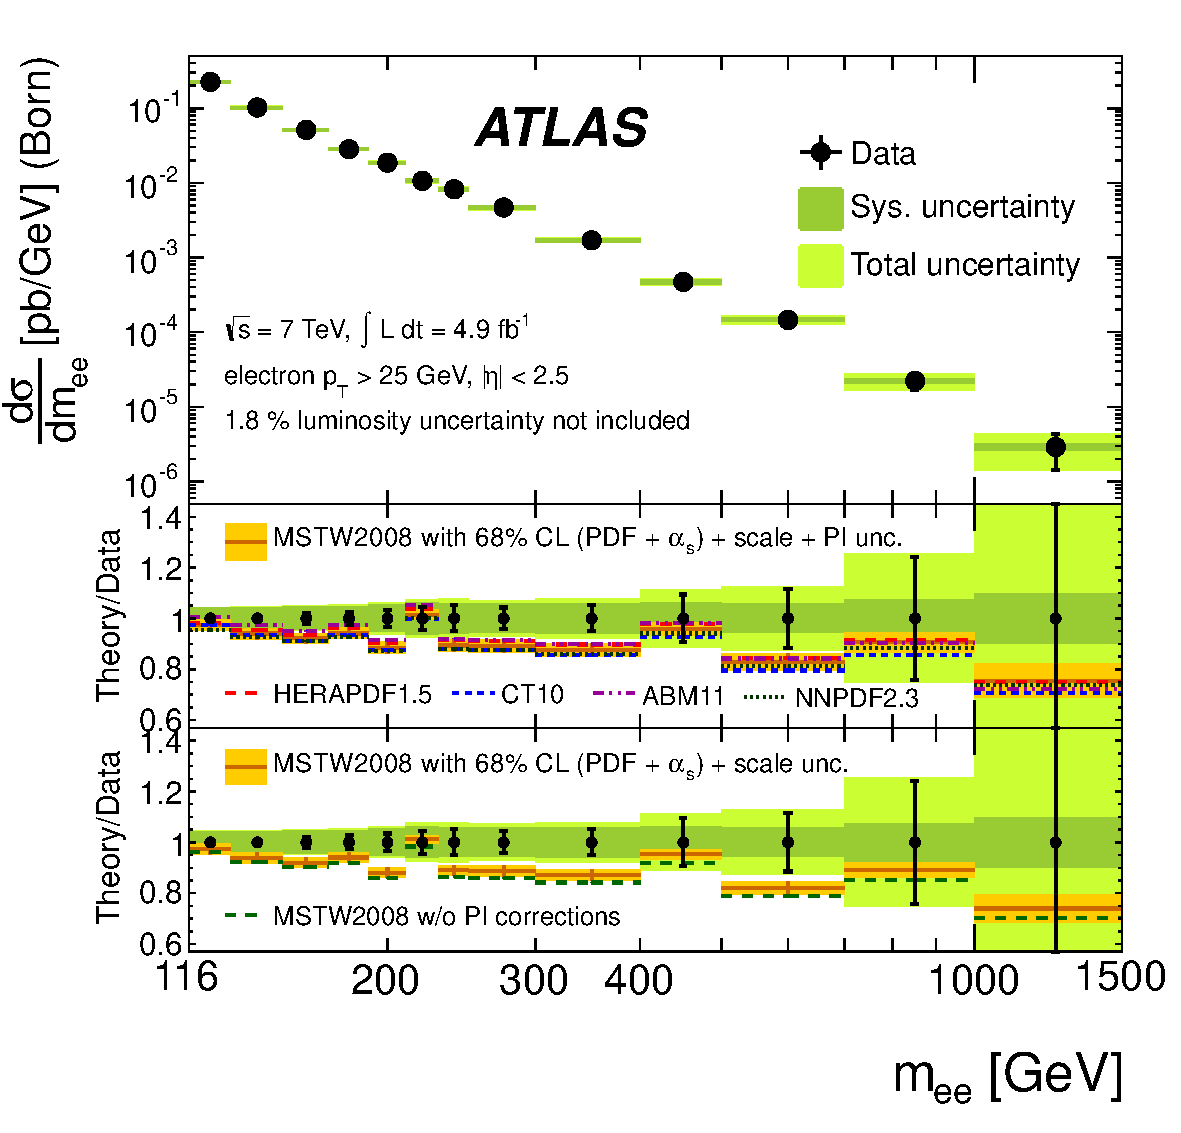
\includegraphics[height=0.3\textheight]{figures/ss-inclboson-drellyan-atlas7tev}
    \caption{Measured differential cross-section at the Born level within the
    fiducial region (electron $\pt > 25 \GeV$ and $|\eta| < 2.5$) with statistical,
     systematic, and combined statistical and systematic (total) uncertainties,
     excluding the 1.8\% uncertainty on the luminosity from ATLAS~\cite{Aad:2013iua}.
     In the upper ratio plot, the photon-induced (PI)
     corrections have been added to the predictions obtained from the MSTW2008,
     HERAPDF1.5, CT10, ABM11 and NNPDF2.3 NNLO PDFs, and for the MSTW2008 prediction
     the total uncertainty band arising from the PDF, $\alpha_s$, renormalisation
     and factorization scale, and photon-induced uncertainties is drawn. The lower
     ratio plot shows the influence of the photon-induced corrections on the
     MSTW2008 prediction, the uncertainty band including only the PDF, $\alpha_s$
     and scale uncertainties.}
    \label{fig:ss-inclboson-drellyan-atlas7tev}
\end{figure}

\begin{figure}[p]
    \centering
    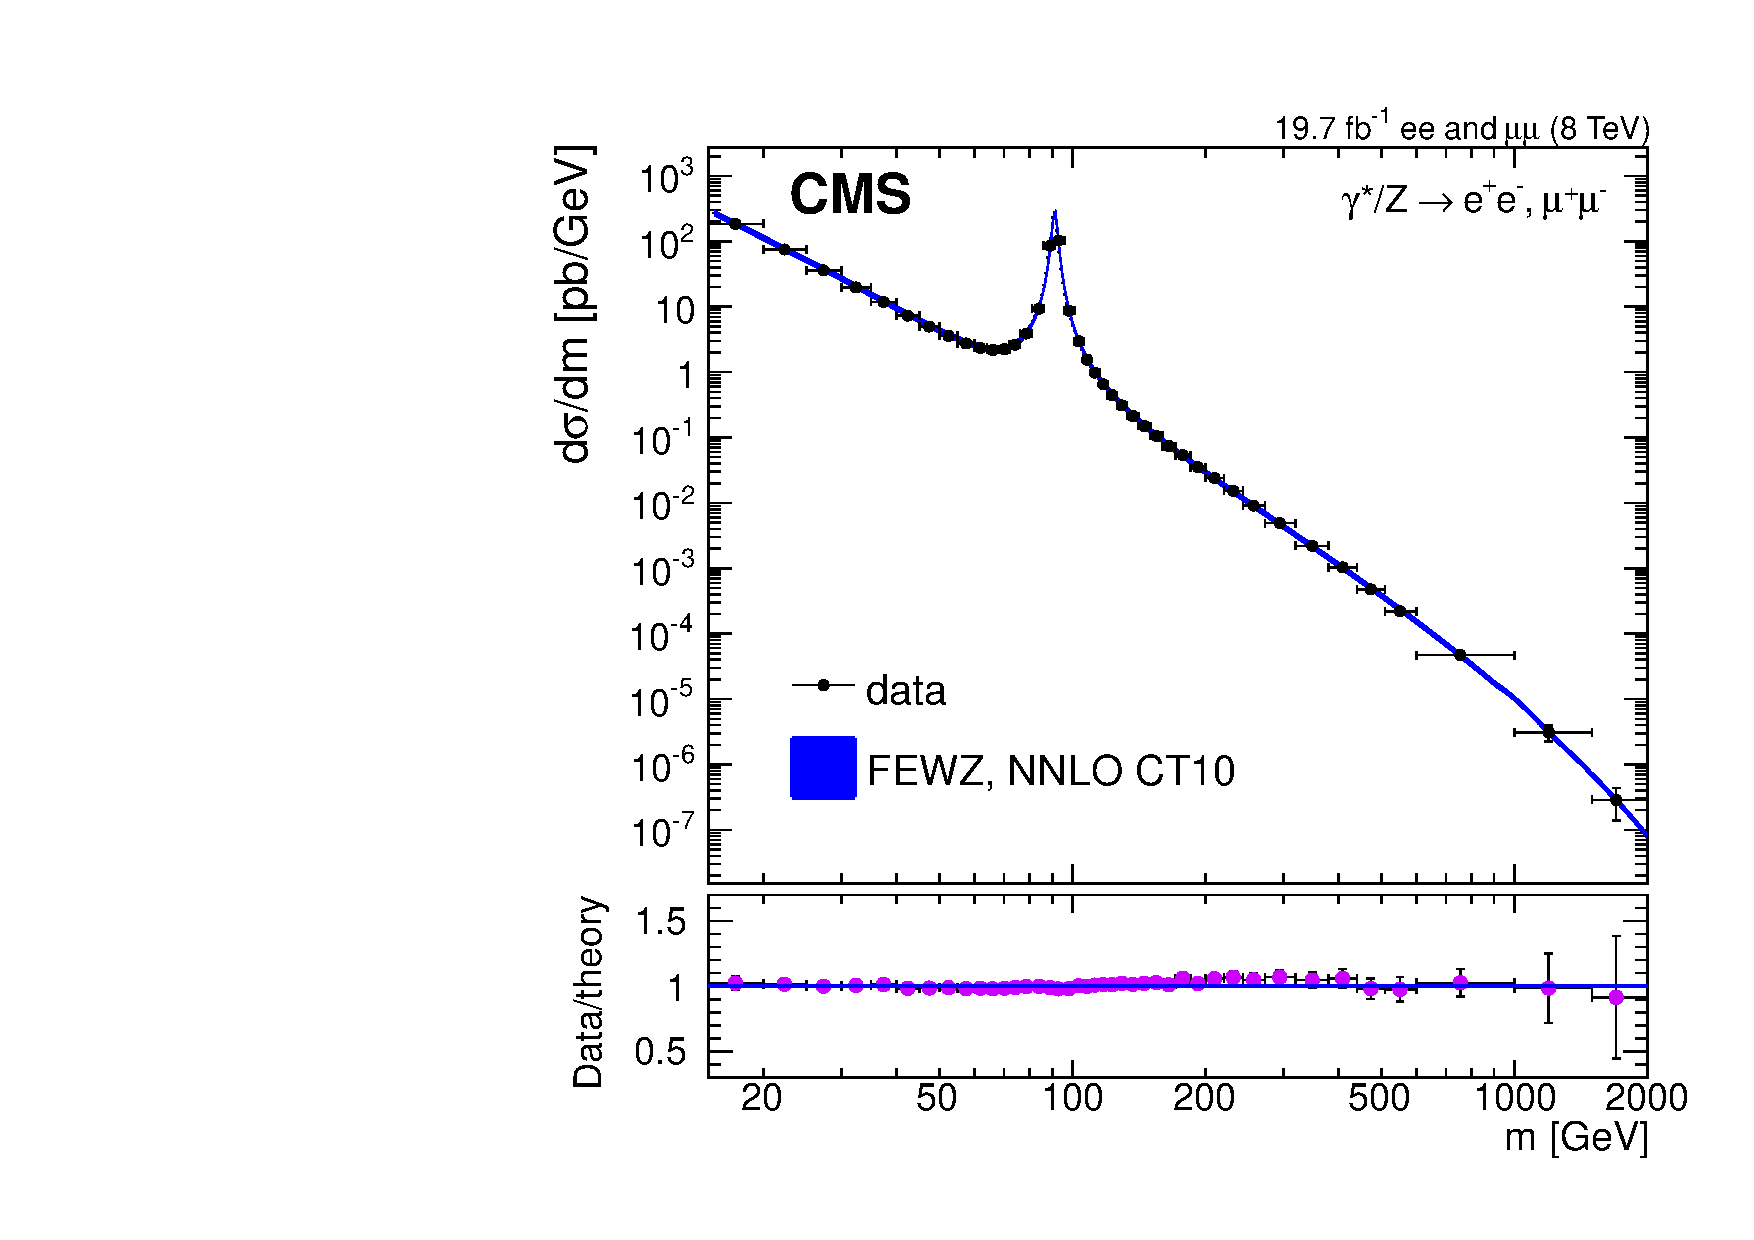
\includegraphics[height=0.3\textheight]{figures/ss-inclboson-drellyan-cms8tev}
    \caption{The DY differential cross section as measured by CMS~\cite{CMS:2014jea} in the combined
dilepton channel and as predicted by NNLO \texttt{FEWZ} 3.1 with CT10 PDF
calculations, for the full phase space.}
    \label{fig:ss-inclboson-drellyan-cms8tev}
\end{figure}

\subsection{Inclusive di-boson production}
\subsubsection{ZZ production}
\label{sss-ZZprod}

%short intro
The production of \ZZ in proton-proton collisions has been one of the first di-boson 
processes measured at the LHC. The SM process is and an important and irreducible
background to resonance searches and Higgs production. The production at leading
order is dominated by quark anti-quark annihilation in the $t$ and $u$-channel,
whereas the $s$-channel process is forbidden in the SM 
(see also Figure~\ref{fig:sss-ZZprod-LOdiagrams}). The gluon fusion process 
contributes about 6\% to the total production cross section. 

%FIGURE LO ZZ DIAGRAM
\begin{figure}[htbp]
  \begin{center}
  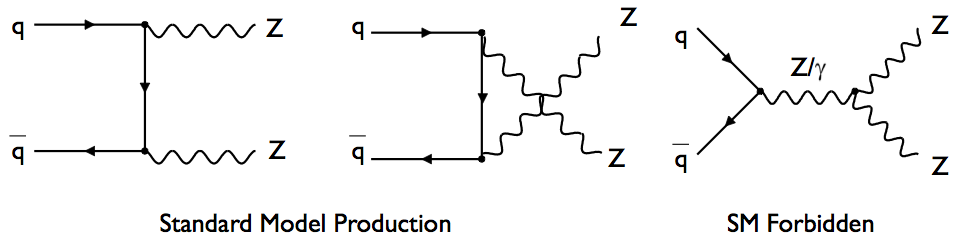
\includegraphics[width=0.9\textwidth]{figures/sss-inclboson-diboson-zzprod-zzdiagram.png}
  \caption{Leading order Feynman diagrams of \ZZ production in the dominant 
  \qqbar\ channel. The \ZZ\ production via the $s$-channel is not allowed in the SM.}
\label{fig:sss-ZZprod-LOdiagrams}
\end{center}
\end{figure}

%decay channels
Precision measurements use the leptonic decay modes of the $Z$ to reduce the impact of
QCD backgrounds. 
The four lepton final state provides an almost background free signature, at the
expense of a relatively small branching ratio 
$BR(ZZ) \to \ll\ll = 0.101^2 \cdot {4 \over 9} = 0.0045$~\cite{PDG}.  
The di-lepton and missing energy channel can exploit the one order of magnitude
higher branching ratio of 
$BR(\ZZ \to \ll\vv) = 0.101 \cdot 0.20 \cdot 2 \cdot {2 \over 3} = 0.0269$, 
at the expense of high background levels.

%analysis CMS and ATLAS.
%ATLAS ZZ 7 TeV~\cite{Aad:2012awa}
%CMS ZZ4l 8 TeV~\cite{Khachatryan:2014dia}
%CMS ZZ4l 7 TeV~\cite{Chatrchyan:2012sga}
%CMS ZZ2l2nu 7+8 TeV~\cite{Khachatryan:2015pba}
The ATLAS collaboration has published results on the $7\TeV$ data-set 
in the $\ll\ll$ and $\ll\vv$ final state~\cite{Aad:2012awa}, and at
$13\TeV$ in the $\ll\ll$ final state~\cite{Aad:2015zqe}. The CMS collaboration
has analysed the full 7 and $8\TeV$ data sets in both 
the $\ll\ll$~\cite{Chatrchyan:2012sga,Khachatryan:2014dia} and 
$\ll\vv$ final state~\cite{Khachatryan:2015pba}.

%Theoretical calculations
% NLO alpha_s arXiv:1105.0020
% NLO alpha_EKW arXiv:1305.5402,arXiv:1307.4331
Theoretical predictions for $\ZZ$ production are available 
at NLO in $\alpha_s$~\cite{arXiv:1105.0020}. In addition, electroweak 
corrections at NLO have been calculated~\cite{arXiv:1305.5402,arXiv:1307.4331}. 

% Z->llll
%Selections
The event selection for the $\ll\ll$ final state requires exactly four leptons 
fulfilling a set of cuts on kinematic quantities. ATLAS and CMS use similar criteria 
as listed in detail in Table~\ref{tab:sss-ZZprod-cuts}. While ATLAS uses $l=e,\mu$,
CMS includes also $\Z\to\tautau$ with subsequent hadronic and leptonic $\tau$
decays. ATLAS uses in addition forward leptons outside the ID tracker
to increase the acceptance by 6\% for electrons and 10\% for muons.
%Backgrounds
The $\ll\ll$ channels offers the cleanest event sample with a background level
of only $2-3\%$ from $\Z+jets$, $\tt$, and di-boson events. 
The background is estimated from data by control regions with looser selection
criteria. 

% Z->llvv
%Selections
Events in the $\ll\vv$ final state are characterized by exactly two leptons 
and missing energy. The event selection requires a leptonic $\Z$ candidate and
missing energy in the event. Both experiments used refined observables of
missing energy with additional information to improve the rejection 
against instrumental background. 
%Backgrounds 
The background level is in the same order
as the signal and substantially higher then for $\ll\ll$ .
Main background sources are $\V+jets$, $\tt$ and di-boson production. 
ATLAS and CMS use data driven techniques to constrain the 
dominant background sources.

% Results at the end?
% xsec
Besides the total cross section for the $pp \to \ZZ$ production process, both
experiments measure also fiducial and differential cross sections. The results are 
summarized in Tabel~\ref{tab:sss-ZZprod-cross-sections}. ATLAS and CMS
use different definitions of the fiducial phase space which needs to be taken into
account to make a direct comparison is possible.
For the total cross section a slightly different mass range for the $\Z$ mass range is
used, where CMS uses a wider range of $60\GeV < \mZ < 120\GeV$ then ATLAS with 
$66\GeV < \mZ < 116\GeV$, which contributes to the difference in the quoted predicted
cross section. Good agreement of experimental and theoretical cross section 
values is observed. 


\begin{table}[htp]
\begin{center}
\resizebox{\textwidth}{!}{
\begin{tabular}{|c|c|c|c|c|c|}
 \hline
 Experiment & decay channel     & \rts & measured $\sigma_{total}$ $[\pb]$                                  & predicted $\sigma_{total}$ $[\pb]$& reference                    \\
 \hline
 ATLAS	     & $\ll\ll$, $\ll\vv$& 7 TeV & {6.7 $\pm$ 0.7 (stat.) $^{+0.4}_{-0.3}$ (syst.) $\pm$ 0.3 (lumi.) }&  6.18$^{+0.25}_{-0.18}$           & \cite{Aad:2012awa}         \\
 CMS	     & $\ll\ll$          & 7 TeV & {6.2 $\pm$ $^{+0.9}_{-0.8}$ (stat.) $^{+0.4}_{-0.3}$ (syst.) $\pm$ 0.1 (lumi.) } & 6.3$\pm 0.4$        & \cite{Chatrchyan:2012sga}  \\
 CMS	     & $\ll\vv$          & 7 TeV & {5.2 $\pm$ $^{+1.5}_{-1.4}$ (stat.) $^{+1.4}_{-1.1}$ (syst.) $\pm$ 0.2 (lumi.) } & 6.1$\pm 0.3$        & \cite{Chatrchyan:2012sga}  \\
 CMS	     & $\ll\ll$          & 8 TeV & {7.7 $\pm$ 0.5 (stat.) $^{+0.5}_{-0.4}$ (syst.) $\pm$ 0.2 (lumi.) } 		        & 7.7$\pm 0.6$        & \cite{CMS:2014xja}         \\ 
 CMS	     & $\ll\vv$          & 8 TeV & {6.9 $\pm$ 0.8 (stat.) $^{+1.8}_{-1.4}$ (syst.) $\pm$ 0.3 (lumi.) }			    & 7.6$\pm 0.3$        & \cite{Chatrchyan:2012sga}  \\% m(ll) > 40GeV, m(vv) > 12GeV
 ATLAS	     & $\ll\ll$			 &13 TeV & {16.7 $\pm$ $^{+2.2}_{-2.0}$ (stat.) $^{+0.9}_{-0.7}$ (syst.) $\pm$ $^{+1.o}_{-0.7}$ (lumi.) }&  15.6$^{+0.4}_{-0.4}$           & \cite{Aad:2015zge}         \\

\hline

\end{tabular}
}
\caption{Summary of measured $\ZZ$ production cross sections from ATLAS and CMS
at 7, 8 and 13 TeV centre-of-mass energies in the four lepton and $\ll\vv$ final state.}
\label{tab:sss-ZZprod-cross-sections}
\end{center}
\label{default}
\end{table}%


%%%%
% THIS MIGHT GO INTO THE SECTION ON TGC
% aTGC
% Spectra ATGC
% charged pT : llvv CMS
% m(llll) : llll CMS
% pT(Z) : llll,llvv ATLAS
Limits on ATGC parameters are determined with differential distributions of the 
invariant di-boson mass (CMS, four lepton channel), 
the transverse momentum of the leading lepton (CMS, $\ll\vv$-channel), or
the transverse momentum of the leading \Z (ATLAS, all channels).
A comparison of the measured and predicted differential cross sections in the 
four-lepton invariant mass is shown from CMS in Figure \ref{fig:sss-inclboson-diboson-zzprod-zzinvmass}.
Also shown is the prediction in the presence of a non-zero value of the anomalous coupling
parameter $f_4^Z=0.015$, which shows an enhancement over the SM value at high 
invariant masses. 

%FIGURE ZZ invariant mass
%1406.0113v2.pdf, FIGURE 5
% https://twiki.cern.ch/twiki/pub/CMSPublic/PhysicsResultsSMP13005/fig5tgcA.pdf
% CMS ZZ 4l 8 TeV
\begin{figure}[htbp]
  \begin{center}
  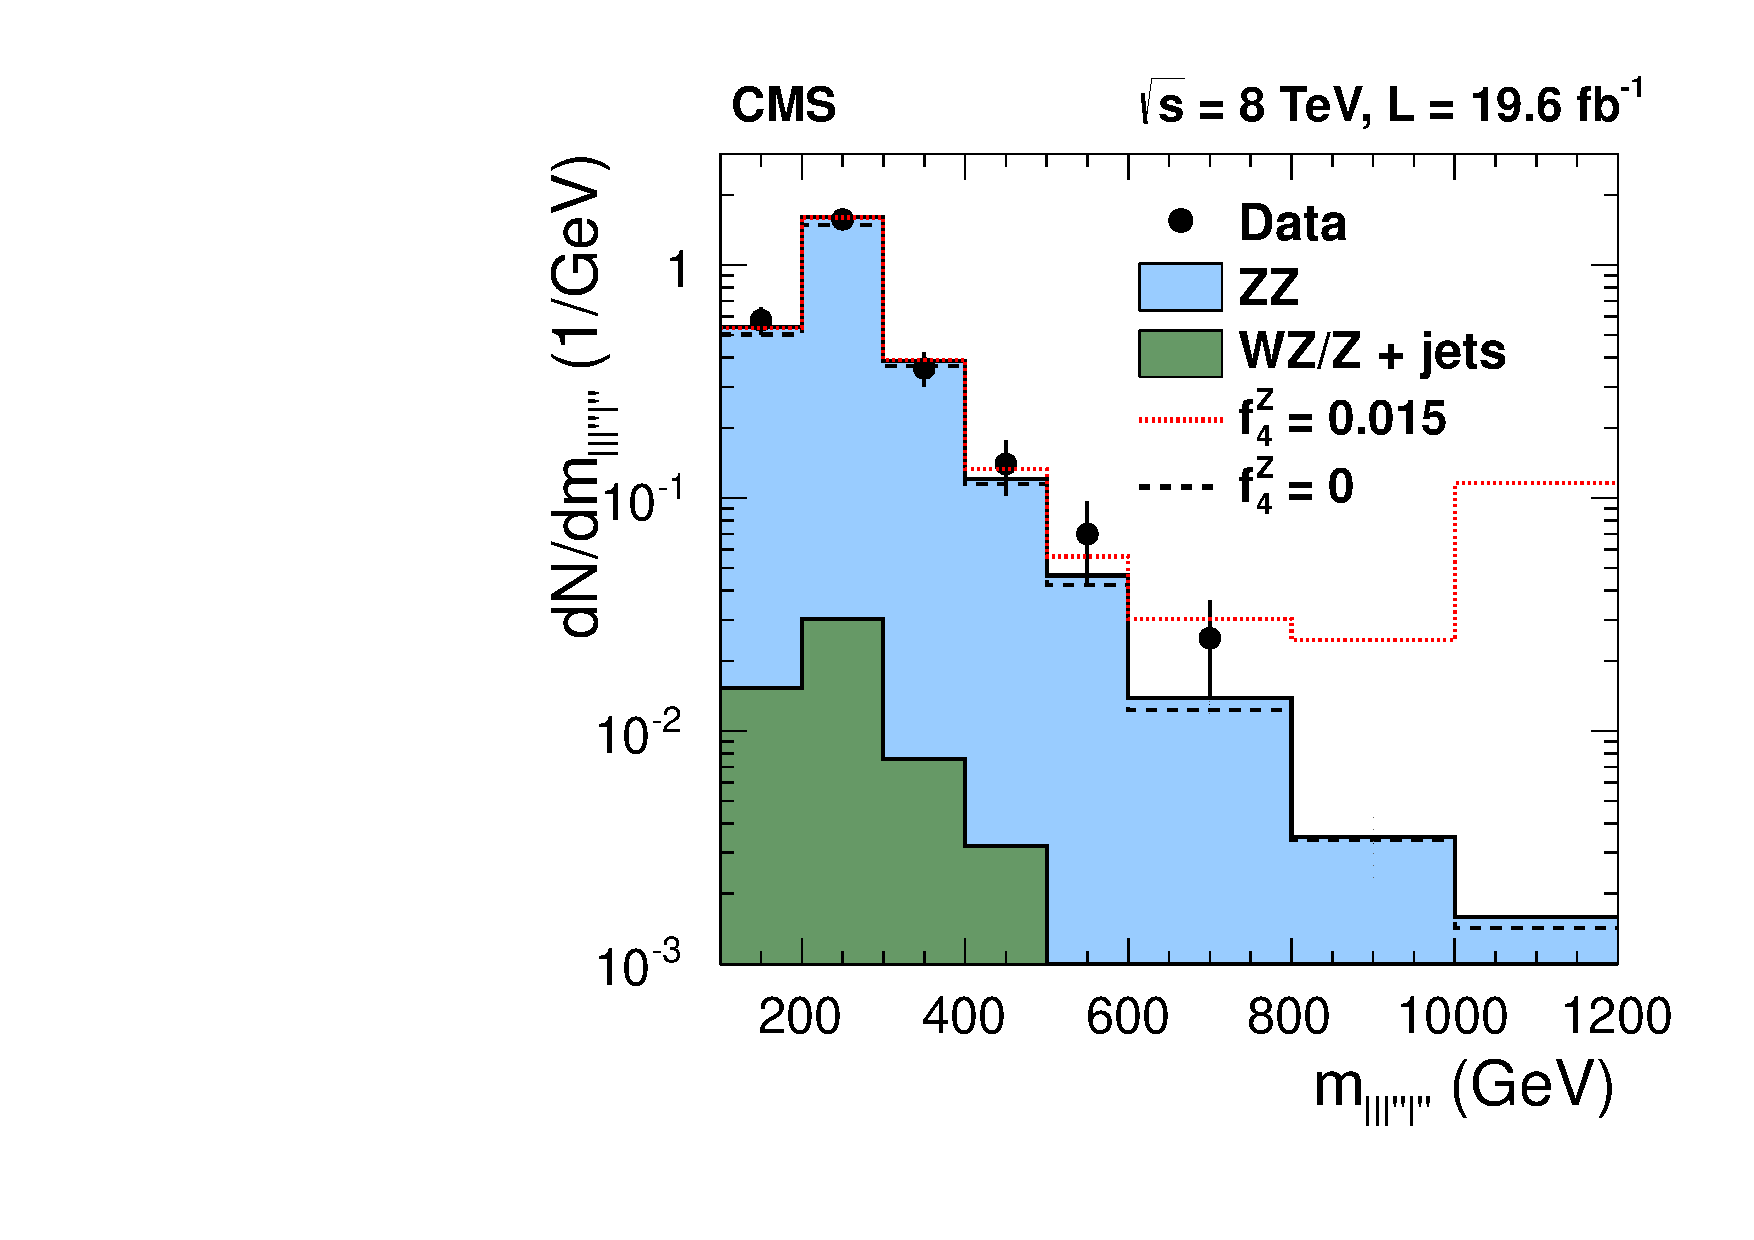
\includegraphics[width=0.9\textwidth]{figures/sss-inclboson-diboson-zzprod-zzinvmass.pdf}
  \caption{ Distribution of the four-lepton reconstructed mass for the combined $4e$, $4\mu$, and $2e2\mu$ channels from CMS~\cite{Khachatryan:2014dia}. Points represent the data, the shaded histogram labeled $\ZZ$ represents the predictions for $\ZZ$ signal, the histograms labeled $\WZ$/$\Z$+jets shows background estimated form data. The dashed and dotted histograms indicate the SM expectation (f4Z = 0) and in the presence of an ATGC (f4Z = 0.015) with all the other anomalous couplings set to zero. The last bin includes all entries with masses above 1000 GeV.
}
\label{fig:sss-inclboson-diboson-zzprod-zzinvmass}
\end{center}
\end{figure}

Both experiment publish 95\% CL limits on ATGC without form factors in the $\ll\ll$ 
and $\ll\vv$ channels. The results are in agreement with the SM and 
summarized in Figure~\ref{fig:sss-inclboson-diboson-zzprod-aTGC_naTGCf} 
taken from Ref. \cite{aTGCplots}. The precision of the LHC results is driven by the steep increase of 
sensitivity with higher centre-of-mass energy
and are about 2 orders of magnitude better compared to the 
combined LEP result~\cite{LEP-comb-2002}.  
% FIGURE COMPARISON OF ZZ NTGC
% https://twiki.cern.ch/twiki/bin/view/CMSPublic/PhysicsResultsSMPaTGC
% M Herndon
% FETCHED 34RD JULY 2015
\begin{figure}[htbp]
  \begin{center}
  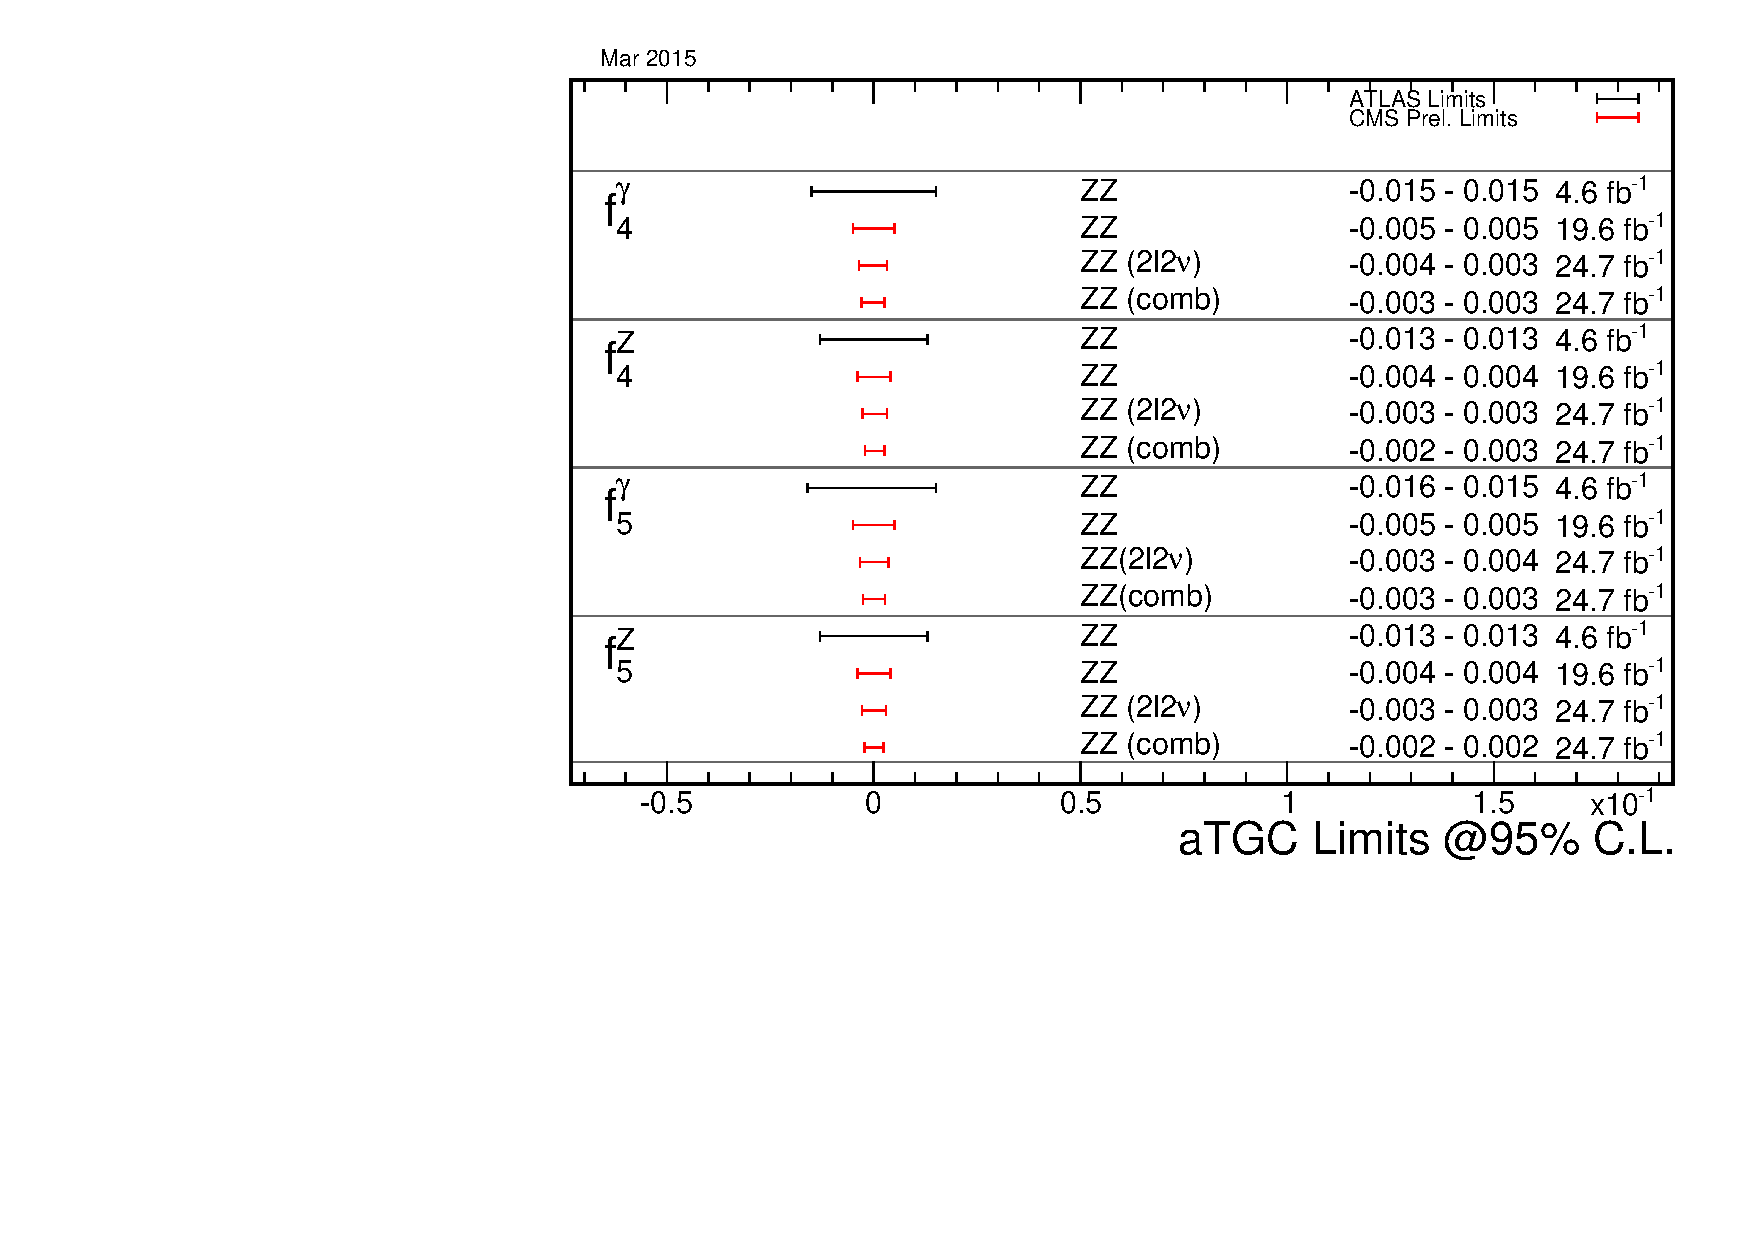
\includegraphics[width=0.9\textwidth]{figures/sss-inclboson-diboson-zzprod-aTGC_naTGCf.pdf}
  \caption{ Comparison of the limits on \ffourv{} and \ffivev{} from ATLAS and CMS in the $\ll\ll$ and $\ll\vv$
  channel at 7 and $8\TeV$.}
\label{fig:sss-inclboson-diboson-zzprod-aTGC_naTGCf}
\end{center}
\end{figure}








%ATLAS ZZ 7 TeV~\cite{Aad:2012awa}
%CMS ZZ4l 8 TeV~\cite{Khachatryan:2014dia}
%CMS ZZ4l 7 TeV~\cite{Chatrchyan:2012sga}
%CMS ZZ2l2nu 7+8 TeV~\cite{Khachatryan:2015pba}

\subsubsection{WZ production}

\label{sss-WZprod}

%short intro
At the LHC, \WZ\ diboson are produced from quark-antiquark initial states at 
leading order (LO) and quark-gluon initial states at next-to-leading order 
(NLO). %~\cite{PhysRevD.65.094041}
%Figure~\ref{fig:LOdiagrams} shows the LO Feynman diagrams for \WZ production from $q\bar{q}'$ initial states. 
The SM allowed $s$-channel diagram has a triple boson vertex and is sensitive to 
ATGC.

%FIGURE LO WZ DIAGRAM
% may include 
% figures/sss-inclboson-diboson-wzprod-wz-s-channel.pdf
% figures/sss-inclboson-diboson-wzprod-wz-t-channel.pdf
% figures/sss-inclboson-diboson-wzprod-wz-u-channel.pdf

%\begin{figure}[htbp]
%  \begin{center}
%  \includegraphics[width=0.9\textwidth]{figures/sss-inclboson-diboson-wzprod-wzdiagram.png}
%  \caption{Leading order Feynman diagrams of \WZ production in the dominant 
%  \qqbar\ channel.}
%\label{fig:sss-WZprod-LOdiagrams}
%\end{center}
%\end{figure}

%decay channels


%analysis CMS and ATLAS.
%ATLAS WZ 8 TEV \cite{Aad:2016ett} 
%ATLAS WZ 7 \TeV~\cite{Aad:2012twa}
% - figure from https://atlas.web.cern.ch/Atlas/GROUPS/PHYSICS/PAPERS/STDM-2012-09/
%CMS WZ at 7+8 \TeV (CMS-PAS-SMP-12-006, to be published)
The ATLAS experiment measured the \WZ\ production cross section in the fully 
leptonic decay channel \ll\lnu\; at $\rts = 7\TeV$~\cite{Aad:2012twa} and $\rts = 8\TeV$~\cite{Aad:2016ett} 
and set limits on charged ATGC.
%Theoretical calculations
% TBD
% WZ->lllv
%Selections
In these analyses the final states involving electrons or muons are considered signal,
whereas boson decays to tau's are considered as background.  
%Backgrounds
The dominant background sources are \Zboson+jet and \ZZ production, accounting for about 40\% of 
the overall background. The overall signal over background ratio is about $4$.
%systematics
The leading systematic uncertainty is related to the data-driven estimation method of the   
background.%, with the dominant Z + jets contributing ($\pm3.8\%$).

% Results at the end
% xsec
The fiducial cross section for the 7 TeV (8 TeV) analysis is defined by $\pt^{\mu,e} > 15\GeV$ for the leptons from the \Zboson\ 
 decay, $\pt^{\mu,e} > 20\GeV$ for the lepton from the \Wboson, $|\eta^{\mu,e}|<2.5$, $\pt^\nu>25\GeV$,
 $|m_ll-m_Z| < 10(25)\GeV$, $M_T^W>20(30)GeV$ and $\Delta R> 0.3$ for the three possible $\ell\ell$ pairings. 
The total cross section requires the mass of the \Zboson\ to be in the range of $66\GeV < |m_Z| < 116\GeV$
to suppress the contribution from $\gamma^*$.
The fiducial and total cross sections are compared to the SM expectation at NLO in Table~\ref{tab:sss-WZprod-xsec}.

\begin{table}[htp]
\begin{center}
\resizebox{\textwidth}{!}{
\begin{tabular}{|c|c|c|c|c|c|}
Experiment & cross section & \rts & measured  & predicted  & reference  \\ \hline
ATLAS & total & 7 GeV & {19$^{+1.4}_{-1.3}$ (stat.) $\pm{0.9}$ (syst.) $\pm$ 0.4 (lumi.) pb}  & {17.6 $^{+1.1}_{-1.0}$ pb} & \cite{Aad:2012twa} \\
ATLAS & total & 8 GeV & {24.3$\pm 0.6$ (stat.) $\pm{0.6}$ (syst.) $\pm{0.4}$ (theo.) $\pm$ 0.5 (lumi.) pb}  & {21.0  $\pm$ 1.6 pb} & \cite{Aad:2016ett} \\
ATLAS & fiducial & 7 GeV & {92 $\pm$ $^{+7}_{-6}$ (stat.) $\pm{4}$ (syst.) $\pm$ 2 (lumi.) fb}  & -- & \cite{Aad:2012twa} \\
ATLAS & fiducial & 8 GeV & {35 $\pm$ $\pm{0.9}$ (stat.) $\pm{0.8}$ (syst.) $\pm$ 0.8 (lumi.) fb}  & {30 $\pm$ $\pm{0.5}$ (PDF) $\pm{0.8}$ (scale) fb} & \cite{Aad:2016ett} \\
\end{tabular}
}
\caption{Summary of measured fiducial and total $\WZ$ production cross sections from ATLAS 
at 7 TeV centre-of-mass energies in the $\ll\lnu$ final state. The fiducial definitions differ from the 7 and 8 TeV analysis. Further, the 7 TeV analysis
quotes the sum for the $e$ and $\mu$ channels, the 8 TeV analysis quotes the combination of channels. Thus, the two fiducial cross sections cannot be 
compared directly.}
\end{center}
\label{tab:sss-WZprod-xsec}
\end{table}%


% unfolded spectra
In Figure~\ref{fig:sss-WZprod-ptZ-det} the differential cross section measured in bins of 
$\pt^Z$ is shown, compared to SM prediction and a set of anomalous TGC couplings. 
The normalized $\pt^Z$ spectrum is unfolded and compared to the NLO calculation of \mcatnlo in 
Figure~\ref{fig:sss-WZprod-ptZ-det}, showing good agreement with the SM.


\begin{figure}[htbp]
  \begin{center}
  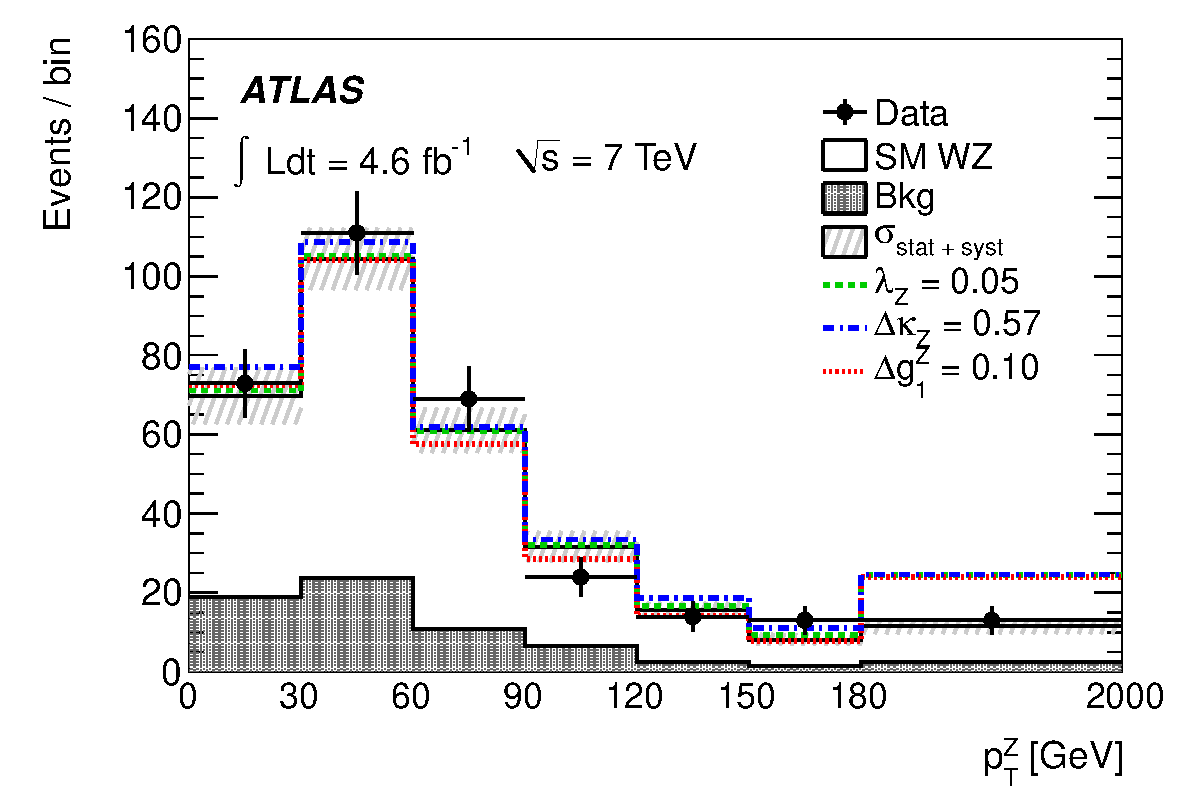
\includegraphics[width=0.45\textwidth]{figures/sss-inclboson-diboson-wzprod-ptZ-det.pdf}
  \caption{ATLAS measurement of the transverse momentum of the \Zboson in \WZ events ($\pt^Z$) compared with the SM prediction at $\rts = 7\TeV$. For illustration calculations for a set of anomalous couplings values are also shown. The full uncertainty contains statistical and systematic uncertainties.}
\label{fig:sss-WZprod-ptZ}
\end{center}
\end{figure}

\begin{figure}[htbp]
  \begin{center}
  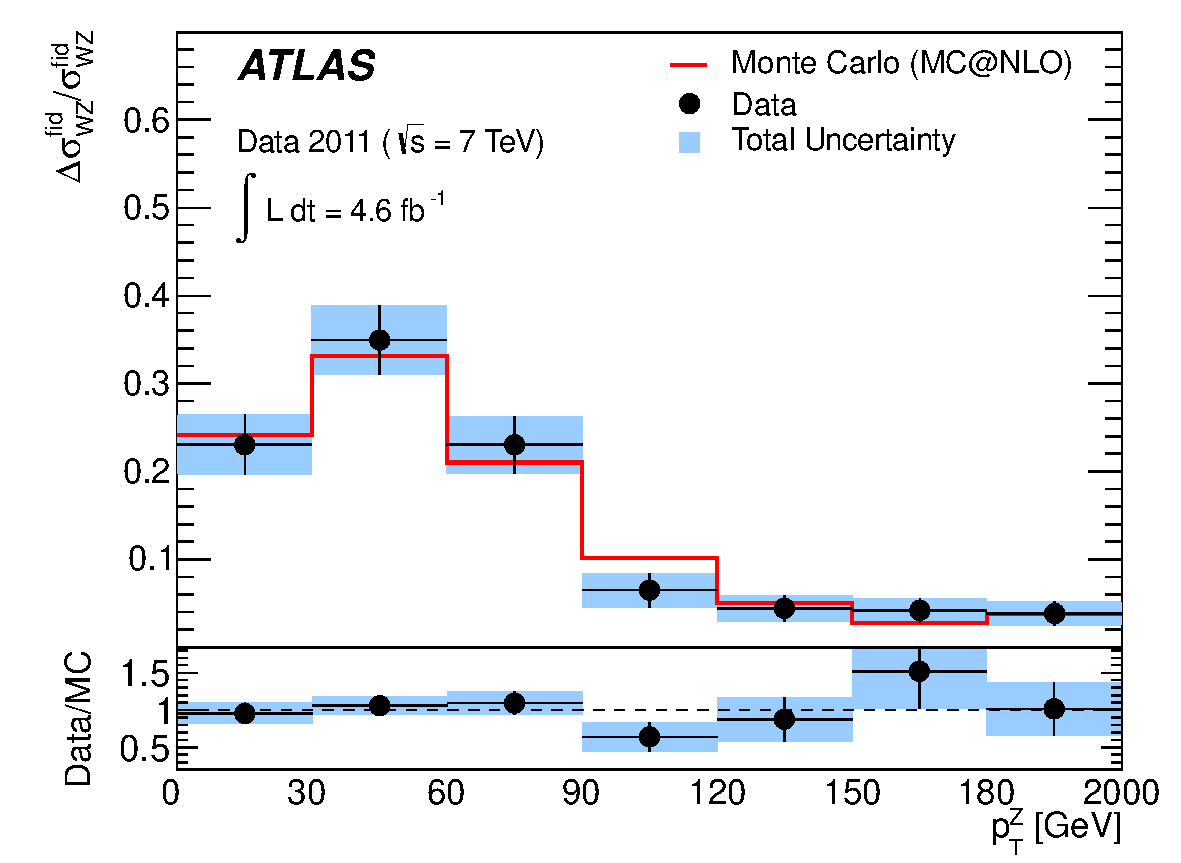
\includegraphics[width=0.45\textwidth]{figures/sss-inclboson-diboson-wzprod-ptZ.pdf}
  \caption{ATLAS measurement of the normalized fiducial cross-sections in bins of $\pt^Z$ compared with the SM prediction at $\rts = 7\TeV$. The full uncertainty contains statistical and systematic uncertainties.}
\label{fig:sss-WZprod-ptZ-det}
\end{center}
\end{figure}


%%%%
% THIS MIGHT GO INTO THE SECTION ON TGC
% aTGC
Limits on the charged ATGC parameters \dkz, \lz\ and \gz\ are extracted from the transverse momentum distribution
of the \Zboson, $\pt^Z$~\cite{Aad:2012twa} or from the transverse mass of the $\Wboson\Zboson$ system~\cite{Aad:2016ett}. 
The ATGC parameter 95\% CL limits using a dipole form-factor with a cut-off of $\Lambda=2\TeV$ and without a form-factor are quoted 
in Table~\ref{tab:sss-WZprod-ATGC} from the more constraining $8\TeV$ data set analysis~\cite{Aad:2016ett}.

%\begin{table}\centering
%\caption{Expected and observed 95\% CL on 
%\dkz, \lz\ and \gz.}
%\label{tab:sss-WZprod-ATGC}
%\begin{tabular}{ccccc}
%\hline
%& $\rts$,  & Observed & Observed & Expected \\
%& & $\Lambda=2$~TeV & no form factor & no form factor\\
%\hline
%$7\TeV$ & $\gz$ & $[-0.074, 0.133]$ & $[-0.057, 0.093]$ & $[-0.046, 0.080]$ \\
%$7\TeV$ & $\dkz$ & $[-0.42, 0.69]$ & $[-0.37, 0.57]$ & $[-0.33, 0.47]$ \\
%$7\TeV$ & $\lz$ & $[-0.064, 0.066]$ & $[-0.046, 0.047]$ & $[-0.041, 0.040]$ \\
%\hline
%\end{tabular}
%\end{table}


\begin{table}\centering 
\begin{tabular}{cccc}
\hline
 $\Lambda$ & Coupling & Expected  & Observed \\
\hline
2 TeV 	& $\gz$ 		& [$-0.023$, $0.055$]  & [ $-0.029$, $0.050$] \\ \\
2 TeV 	& $\dkz$ 	& [$-0.17$, $0.25$]    & [$-0.19$, $0.30$] \\
2 TeV 	& $\lz$ 	& [$-0.016$, $0.016$]  & [$-0.016$, $0.016$] \\
\hline
\end{tabular}
\caption{Expected and observed 95\% CL on \dkz, \lz\ and \gz\; for a cut-off parameter $\Lambda = 2\TeV$ and $\Lambda = \infty$.}
 \label{tab:sss-WZprod-ATGC}
\end{table}
 

% WZ->llqq ????











\subsubsection{WW production}
\label{sss-WWprod}

%short intro
The \WW\ production process has the highest production cross section
among the massive vector di-boson processes. It is also an important
background process to Higgs production and to searches for new physics.
%analysis CMS and ATLAS.
%    ** ATLAS (5.6ifb, 7TeV, TGC), Phys. Rev. D 87, 112001 (2013), http://arxiv.org/abs/1210.2979
%	    ATLAS (20ifb 8TeV), https://atlas.web.cern.ch/Atlas/GROUPS/PHYSICS/CONFNOTES/ATLAS-CONF-2014-033/ 
%    ** CMS (7 TeV, 5 fb-1, TGC)  WW cross section in the lvlv channel at 7 TeV  http://arxiv.org/abs/1306.1126
%    ** CMS (8 TeV, 3.5 fb-1 WW, 5.3 fb-1 ZZ) , Phys. Lett. B 721 (2013) 190, WW and ZZ at 8 TeV, http://arxiv.org/abs/1301.4698 
%	    CMS (20ifb, 8TeV), submitted to EPJC,  http://arxiv.org/abs/1507.03268
ATLAS and CMS, observed the \WW\ production process in 
the fully leptonic channel and published results for 7 TeV 
(ATLAS~\cite{ATLAS:2012mec}, CMS~\cite{Chatrchyan:2013yaa}) and
8 TeV (CMS~\cite{Chatrchyan:2013oev}) center-of-mass energy. 
%decay channels
Three final states, namely $ee$, $\mu\mu$, and $e\mu$ are included in the analyses. 
The contribution from leptonically decaying $\tau$ leptons is included in the signal
definition. Although the production cross section is relatively high, the signature of two opposite 
sign leptons and missing transverse energy is shared with many processes and a careful
control of the backgrounds is necessary to achieve a precise measurement.

%Theoretical calculations
% TBD -> General section about theoretical calculations?

%Selections
Candidate $\WW$ events are selected by requiring two oppositely-charged leptons 
accompanied with large \MET. 
%Backgrounds
The dominant background sources are \ttbar\; and single top quark, 
$\W/$+jets, followed by $\Zzero/\gamma^{*}$+jets production.
To suppress the dominant \ttbar\; background, events with one or more jets are rejected.   
Additional requirements on \MET\ and the use of top quark-taggers further reduce the residual background
%ATLAS: 685 WW, 275 background => b / (s+b) = 29%
%CMS: 824WW, 369 background => b / (s+b) = 31%
to about 30\%.  
%systematics
The dominant systematic uncertainty is related to the jet veto efficiency 
and estimated to be about 5\% for the \WW\, production. 
The experiments quote a theoretical uncertainty on the signal acceptance due to 
variations of the parton distribution functions and renormalization and factorization 
scales in the range of 1-2\%.

% Results at the end
% total xsec
% ATLAS 7TeV 4.6 ifb: xsec(WW) = 51.9 +- 2.0 (stat) +- 3.9 (sys) +- 2.0 (lum) pb
%                     xsec_theo(WW) = 44.7 +2.1 -1.9 pb
% CMS 7TeV 4.9 ifb: xsec(ww) = 52.4 +- 2.0 (stat) +- 4.5 (syst) +- 1.2 (lum) pb
%                   xsec_theo(WW) = 47.0 +- 2.0 pb
% CMS 8TeV 5ifb: xsec(WW) = 69.9 +- 2.8 (stat) +- 5.6 (sys) +- 3.1 (lum) pb
%                xsec_theo(WW) = 57.3 +2.3 -1.6 pb (not including H ~ 4%)

% definition of total xsecs might differ (inclusion of higgs or not).
Both ATLAS and CMS provide a measurement of the total cross section for the process $pp \rightarrow \WW$
and compare to theoretical calculations. The Higgs process contributes with about 4\% to the total 
cross section and has not been taken into account in the comparison to the SM predictions.
The total cross section results are summarized in Table~\ref{tab:sss-WWprod-xsec}.
A good agreement between the experiments for the measured cross section as well as for the theoretical predictions
is observed.
% fiducial xsec
A normalized differential measurement of the fiducial cross section in bins of $\pt$ of the leading lepton is presented by ATLAS,
as shown in Figure~\ref{fig:sss-WWprod-pt-fiducial}. The unfolded spectrum is in agreement with the SM prediction.

\begin{table}[htp]

\begin{center}
\resizebox{\textwidth}{!}{
\begin{tabular}{|c|c|c|c|c|c|}
Experiment & cross section & \rts\; [TeV] & measured [pb]  & predicted [pb] & reference  \\ \hline
ATLAS & total & 7 & {51.9 $\pm 2.0$  (stat.) $\pm$ ${3.9}$ (syst.) $\pm$ 2.0 (lumi.) }  & {44.7 $^{+2.1}_{-1.9}$ } & \cite{ATLAS:2012mec} \\
CMS & total & 7 & {52.4 $\pm 2.0$  (stat.) $\pm$ ${4.5}$ (syst.) $\pm$ 1.2 (lumi.) }  & {47.0 $\pm 2.0$ } & \cite{Chatrchyan:2013yaa} \\
CMS & total & 8 & {69.9 $\pm 2.8$  (stat.) $\pm$ ${5.6}$ (syst.) $\pm$ 3.1 (lumi.) }  & {57.3 $^{+2.3}_{-1.6}$} & \cite{Chatrchyan:2013yaa} \\
\end{tabular}
}
\caption{Summary of measured fiducial and total $\WW$ production cross sections from ATLAS and CMS 
at 7 and 8 TeV center-of-mass energies in the $\lnu\lnu$ final state.}
\end{center}
\label{tab:sss-WWprod-xsec}
\end{table}%

% unfolded spectra
% https://atlas.web.cern.ch/Atlas/GROUPS/PHYSICS/PAPERS/STDM-2012-01/fig_07.pdf
% 
\begin{figure}[htbp]
  \begin{center}
  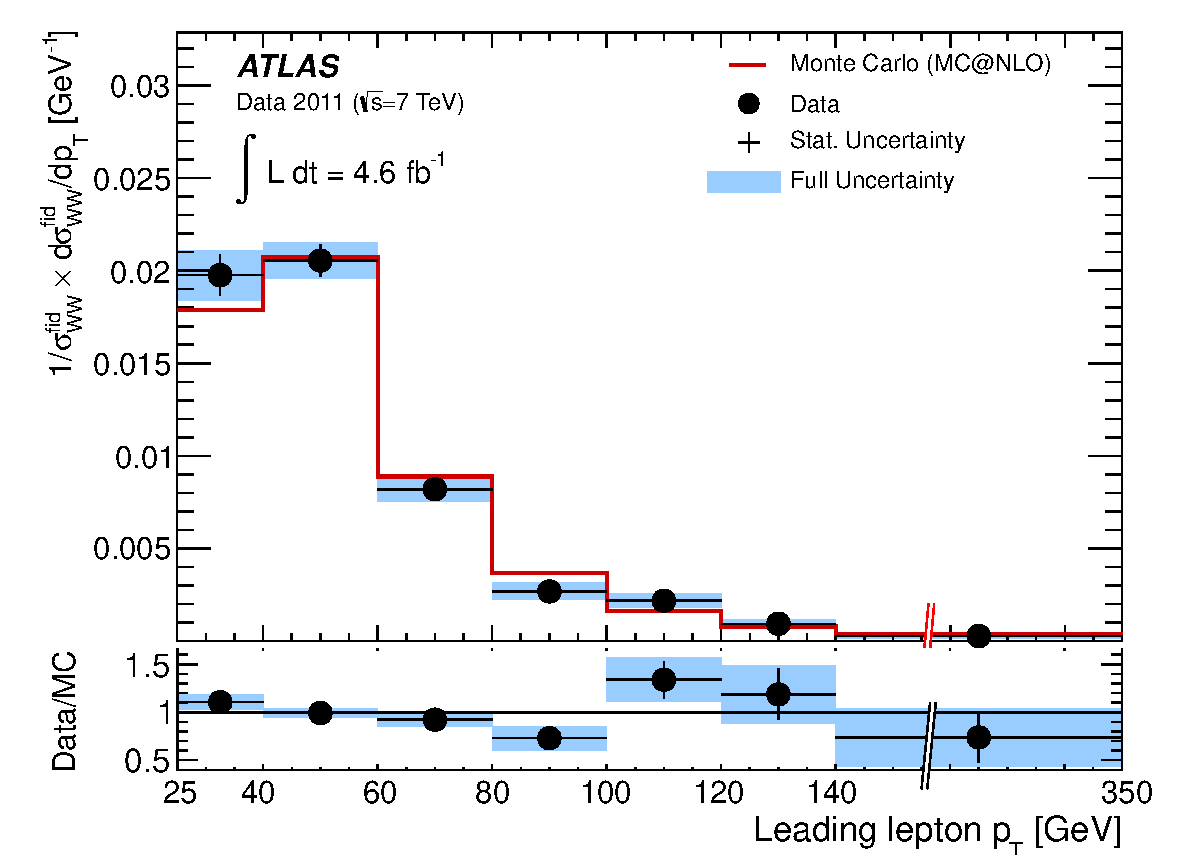
\includegraphics[width=0.45\textwidth]{figures/sss-inclboson-diboson-wwprod-pt-fiducial.pdf}
  \caption{ATLAS measurement~\cite{ATLAS:2012mec} of the transverse momentum of the leading lepton in \WW events compared with the SM prediction at $\rts = 7\TeV$. The full uncertainty contains statistical and systematic uncertainties.}
\label{fig:sss-WWprod-pt-fiducial}
\end{center}
\end{figure}


%%%%
% THIS MIGHT GO INTO THE SECTION ON TGC
% aTGC
The leading lepton $\pt$ spectrum of the \WW process is sensitive to anomalous gauge boson coupling parameters
\dkg,  \dkz, \lg, \lz, and \dgz. Both ATLAS and CMS quote limits in the LEP 
parametrization~\cite{Gounaris:1996rz} that introduces $SU(2) \times U(1)$ gauge invariance 
constraints to reduce the number of free parameters to \dgz,  \dkg, and \lz. The obtained limits assuming 
no form factor are compared for both expected and measured 95\% CL limits in Table~\ref{tab:sss-WZprod-ATGC}.

\begin{table}\centering
\begin{tabular}{cccc}
\hline
& Observed (CMS) & Observed (ATLAS) & Expected (ATLAS)\\
\hline
$\dgz$ & $[-0.095, 0.095]$ & $[-0.039, 0.052]$ & $[-0.039, 0.052]$ \\
$\dkg$ & $[-0.21, 0.22]$ & $[-0.14, 0.14 ]$ & $[-0.13, 0.13]$ \\
% ATLAS DKZ limits converted to DKG with DKG = c2/s2(DG1-DKZ) = 3.3252 * (-DKZ) [DG1 == 0]
$\lz$ & $[-0.048, 0.048]$ & $[-0.062, 0.059]$ & $[-0.060, 0.059]$ \\
\hline
\end{tabular}
\caption{Expected and observed 95\% CL limits on the ATGC parameters 
\dkg, \lz\ and \dgz\; in the LEP parametrization derived from the leading lepton $\pt$ spectrum in \WW production at 7 TeV (ATLAS~\cite{ATLAS:2012mec}, CMS~\cite{Chatrchyan:2013yaa}). No form-factor is applied to the ATGC parameters.}
\label{tab:sss-WZprod-ATGC}
\end{table}







\subsubsection{Semi-leptonic VV production}
\label{sss-VVprod}

%analysis CMS and ATLAS.
%	[Chatrchyan:2012bd] CMS (7TeV, dijet), Eur. Phys. J. C 73 (2013) 2283, http://arxiv.org/abs/1210.7544 
%	[Chatrchyan:2014aqa] OPTIONAL CMS (8TeV, bjet, (Z(W/Z) -> bb (lv/ll))), Eur. Phys. J. C 74 (2014) 2973, http://arxiv.org/abs/1403.3047 
%	[Aad:2014mda] ATLAS, JHEP01(2015)049, http://arxiv.org/abs/1410.7238


%intro
The cross sections for \WW\; and \WZ\; production have been measured also in the 
semileptonic decay channel in the \WVlvqq\; final state with $\V=\Wpm,\Zzero$.
The semileptonic final state has a relatively large background mainly from \V\; production
with associated jets compared to the fully leptonic decay channels, but offers a 
substantially larger branching fraction. The increased statistics of signal events 
at high partonic centre of mass compared to the fully leptonic 
decay modes enhances specifically the sensitivity to aTGC.
ATLAS and CMS have published measurements of the
inclusive production cross section $\WW+\WZ$ and set limits on charged aTGC 
with the full data set of the $\rts=7\TeV$ run~\cite{Aad:2014mda,Chatrchyan:2012bd}.

%decay channels
Both analysis use the semileptonic decay channel with an electron or muon
and two jets in the final state.
%Selections
The event selection sets requirements 
on the lepton \pT, the \MET, di-jet invariant mass, and the event topology. 
The signal fraction of \WW+\WZ in the event sample after selection is only about 1\%, 
and no further selection criteria are applied to distinguish between 
\WW\; and \WZ\; production.
%Backgrounds
The dominant background from \Z/\W+jets production is constrained with data driven methods,
folowed by the sub-leading background contributions from $\ttbar$ and multi-jet production. 
%systematics
The cross-section is extracted with a simultaneous fit of the di-jet invariant mass 
spectrum comprising the signal and background components. In Figure~\ref{fig:sss-lvjjVVprod-mjj} the di-jet invariant
mass spectrum and the extracted signal after background subtraction from Ref.~\cite{Aad:2014mda} is shown. 
The largest systematic uncertainty is related to the modelling of the \Z/\W+jets background
with about 20\% on the cross section.

\begin{figure}[th!]
  \begin{center}
     \subfigure[]
              {
              %https://atlas.web.cern.ch/Atlas/GROUPS/PHYSICS/PAPERS/STDM-2012-22/fig_03a.pdf
     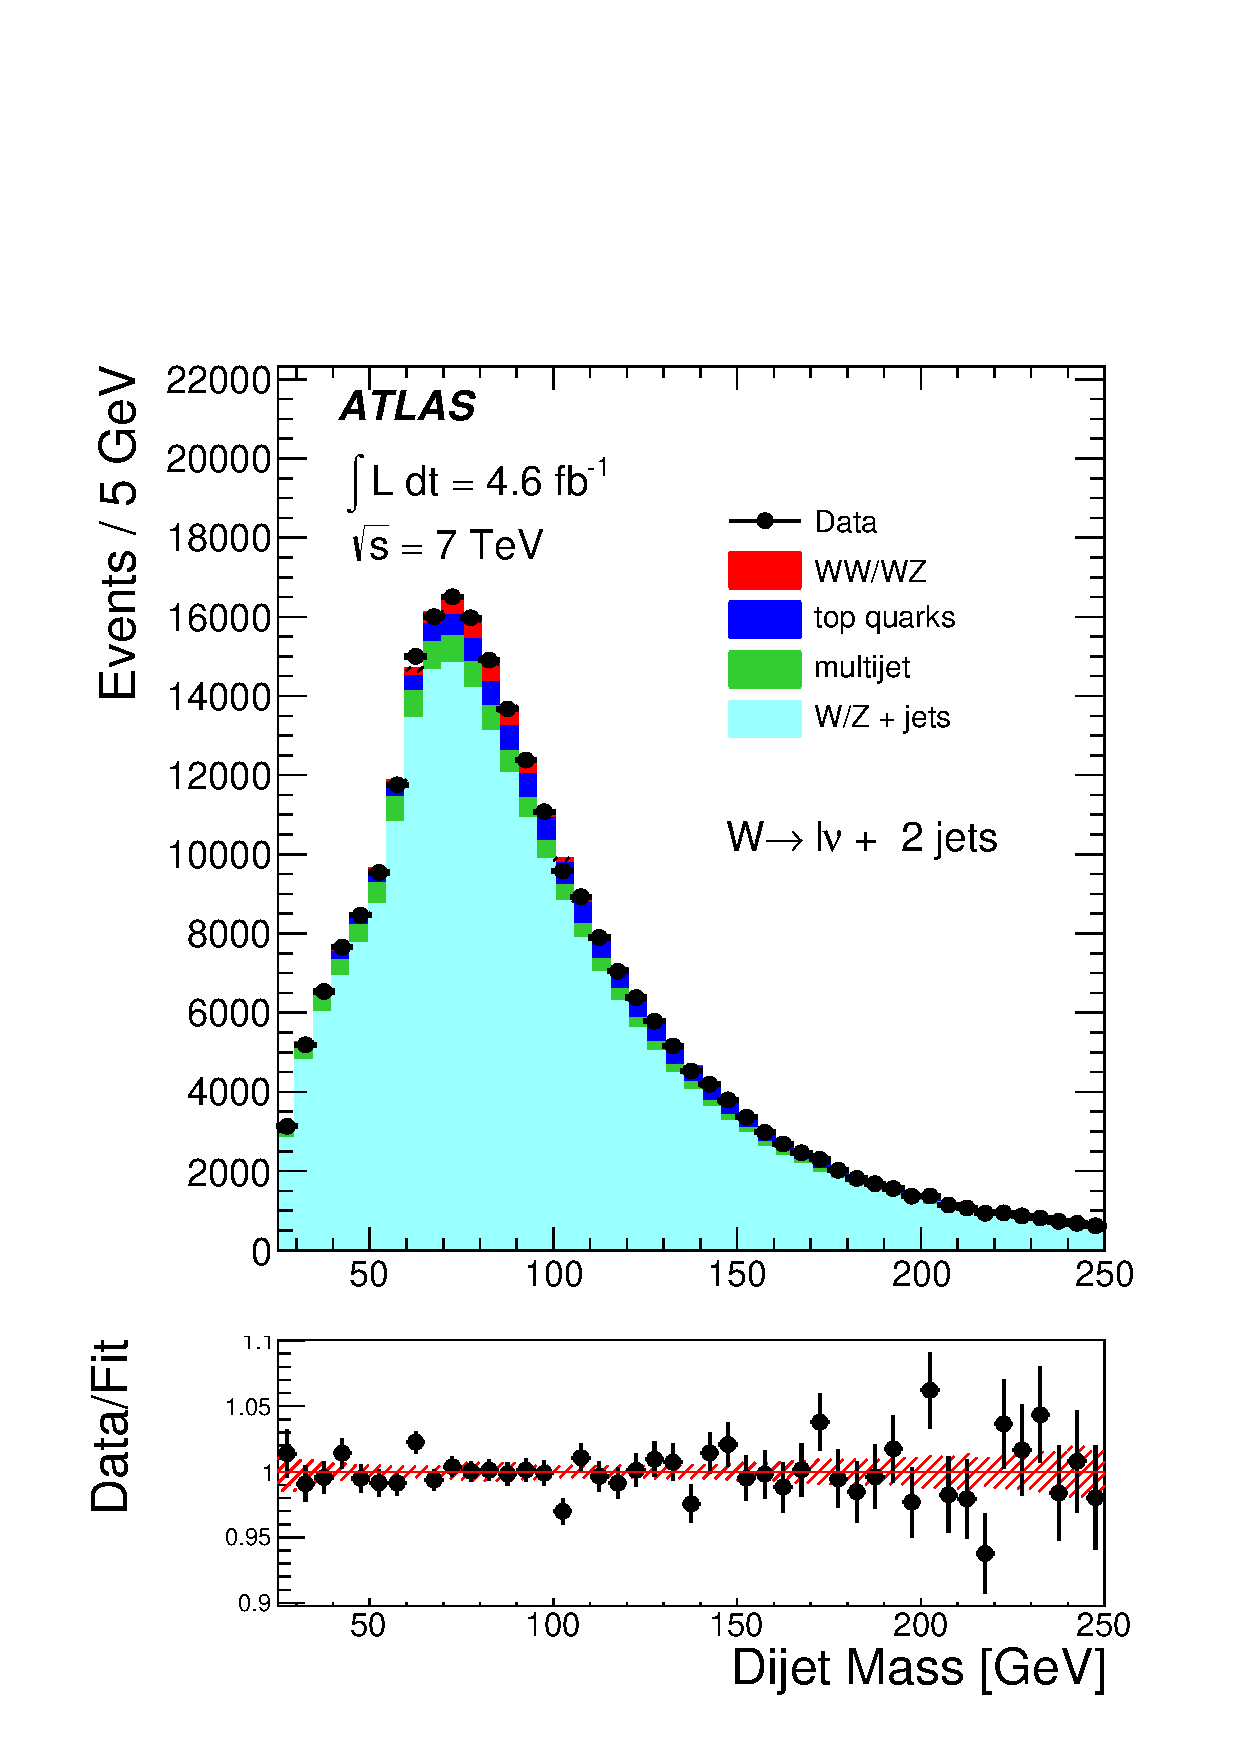
\includegraphics[width=0.485\textwidth]{figures/sss-inclboson-diboson-lvjjVVprod-mjjall.pdf}\label{fig:sss-lvjjVVprod-mjjall}
              }
    \subfigure[]
              {
              %https://atlas.web.cern.ch/Atlas/GROUPS/PHYSICS/PAPERS/STDM-2012-22/fig_03b.pdf
     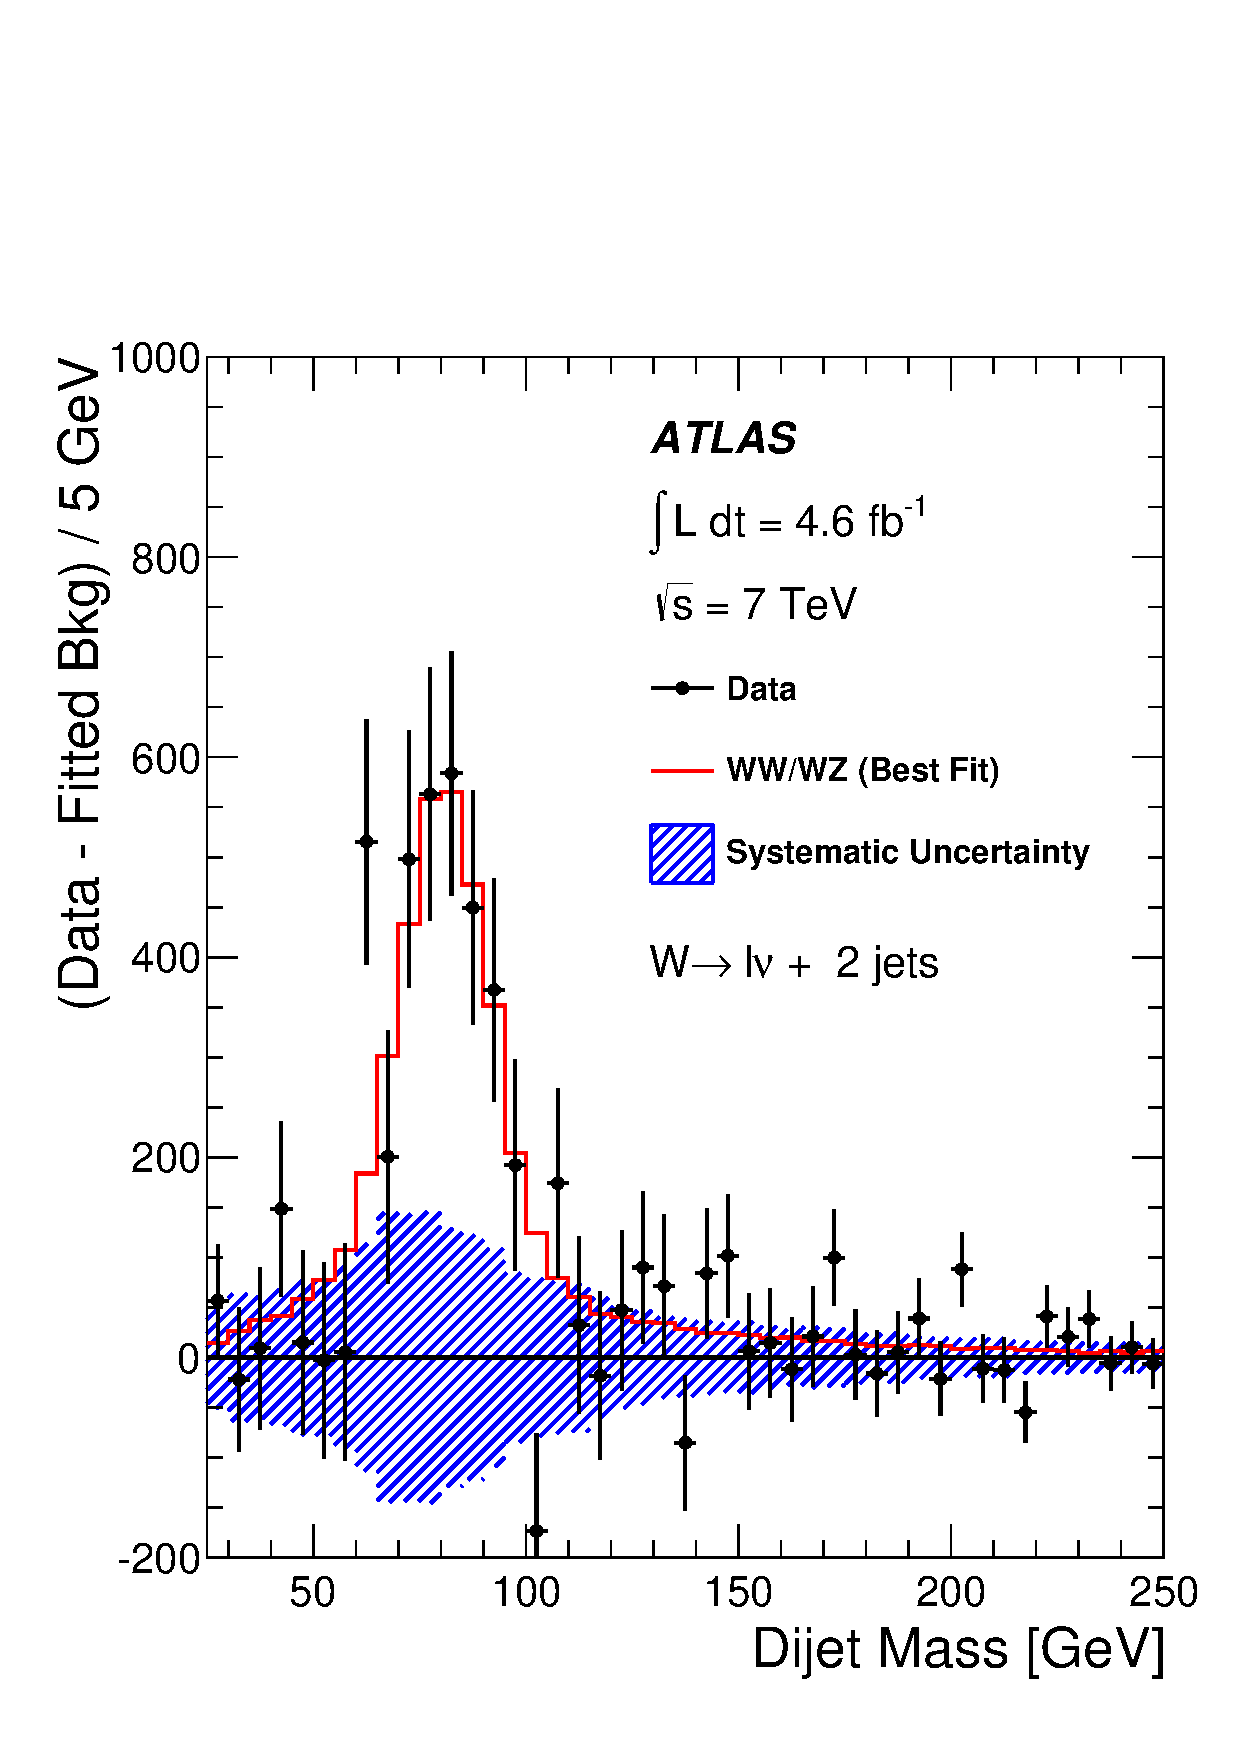
\includegraphics[width=0.485\textwidth]{figures/sss-inclboson-diboson-lvjjVVprod-mjjsig.pdf}\label{fig:sss-lvjjVVprod-mjjsig}
              }
   \end{center}
\vspace{-20 pt}
     \caption{(a) The di-jet invariant mass spectrum for the sum of electron and muon channels, (b) the distribution of the background subtracted data. The lower panel shows that ratio of data and total fit result.}
\label{fig:sss-lvjjVVprod-mjj}
\end{figure}

% Results at the end
The measured and predicted cross sections are compared in Table~\ref{tab:sss-lvjjVVprod-xsec}. 
\begin{table}[htdp]
\begin{center}
\resizebox{\textwidth}{!}{
\begin{tabular}{|c|c|c|c|c|c|}
Experiment & cross section & \rts & measured  & predicted  & reference  \\ \hline
ATLAS & total & 7 GeV & {68$\pm{7}$ (stat.) $\pm{19}$ (syst.+lumi.) pb}  & {61.1  $\pm$ ${2.2}$ pb} & \cite{Aad:2014mda} \\
CMS & total & 7 GeV & {68.9 $\pm$ $\pm{8.7}$ (stat.) $\pm{9.7}$ (syst.) $\pm$ 1.5 (lumi.) pb}  & 65.6 $\pm$ 2.2 pb & \cite{Chatrchyan:2012bd} \\
\end{tabular}
}
\caption{Summary of measured total $\WZ+\WW$ production cross sections from ATLAS and CMS
at 7 TeV centre-of-mass energies in the \WVlvqq\; final state.}
\end{center}
\label{tab:sss-lvjjVVprod-xsec}
\end{table}

%TGC
% ATLAS, LEP scenario:
% l_z = l_gamma : obs [-0.039, 0.040], exp [-0.048, 0.047]
% dk_gamma : obs [-0.21,0.22], exp [-0.23,0.25]
% dg1z : obs [-0.055, 0.071], exp [-0.072, 0.085]
%
% CMS: (HISZ, but could be LEP scenario)
% l : obs [-0.038, 0.030]
% dk_gamma : obs [-0.11, 0.14]

To extract limits on aTGC parameters the transverse momentum of the di-jet system $\pt(jj)$ is used 
by ATLAS and CMS. The resulting 95\% CL limits are listed in Table~\ref{tab:sss-lvjjVVprod-ATGC}. The ATLAS
limits use the LEP scenario~\cite{Gounaris:1996rz}, while the CMS limits are derived in the HISZ~\cite{HAGIWARA1992353,PhysRevD.48.2182} scenario. The achieved precision is comparable to the fully leptonic
channel.

\begin{table}\centering
\caption{Expected and observed 95\% CL on \dkg, $\lz=\lg$ and \dgz in measured in the 
\WVlvqq\; final state from the ATLAS~\cite{Aad:2014mda} and CMS~\cite{Chatrchyan:2012bd} 
collaborations.}
\label{tab:sss-lvjjVVprod-ATGC}
\begin{tabular}{cccc}
\hline
 & CMS & \multicolumn{2}{c}{ATLAS}   \\ 
 & Observed & Observed & Expected \\
\hline
$\lz=\lg$ & $[-0.038, 0.030]$ & $[-0.039, 0.040]$ & $[-0.048, 0.047]$ \\
$\dkg$ 	  & $[-0.11, 0.14]$ & $[-0.21,0.22]$ & $[-0.23,0.25]$ \\
$\dgz$   & \--- & $[-0.055, 0.071]$ & $[-0.072, 0.085]$ \\
\hline
\end{tabular}
\end{table}


% mentioning of (Z(W/Z) -> bb (lv/ll))
A  measurement of the \WZ\; and \ZZ\; production cross sections 
at $\rts=8\TeV$ with a data set of $18.9\ifb$ 
in the semileptonic final state with two $b$-quark jets from the \Zzero 
and $\ll$, $\vv$ or $\lnu$ has been published by CMS~\cite{Chatrchyan:2014aqa}, so 
far the only published results at 8 \TeV\; for these channels.
The measured cross sections 
($\sigma(pp\to\WZ)=30.7\pm 9.3$(stat)$\pm 7.1$(syst)$\pm 4.1$(theo)$\pm 1.0$(lumi)$\pb$
and
$\sigma(pp\to\ZZ)=6.5\pm 1.7$(stat)$\pm 1.0$(syst)$\pm 0.9$(theo)$\pm 0.2$(lumi)$\pb$
) 
are consistent with theoretical calculation at
NLO in $\alpha_s$ 
(
$\sigma(pp\to\ZZ) = 22.3\pm 1.1\pb$ and $\sigma(pp\to\ZZ)=7.7\pm 0.4\pb$
), 
with the precision being still statistically limited. 

% unfolded spectra
% https://atlas.web.cern.ch/Atlas/GROUPS/PHYSICS/PAPERS/STDM-2012-01/fig_07.pdf
% 
%\begin{figure}[htbp]
%  \begin{center}
%  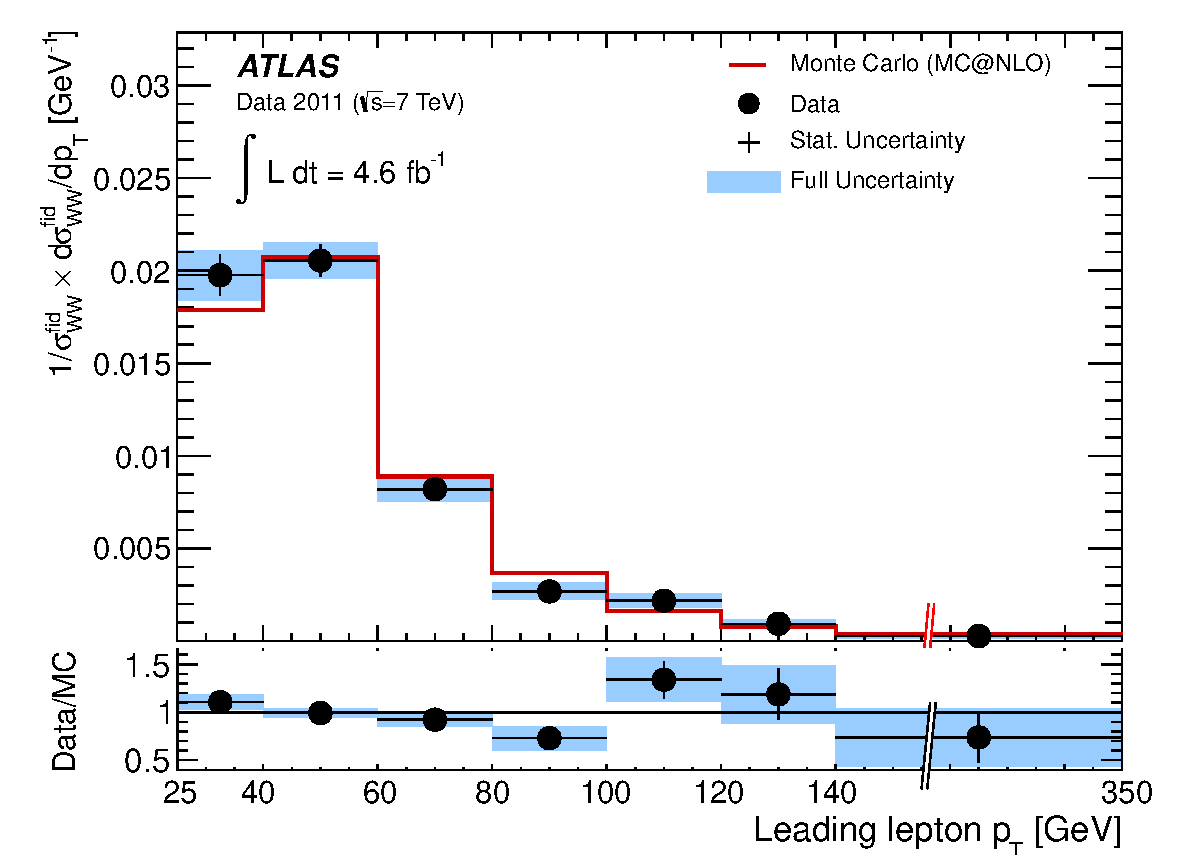
\includegraphics[width=0.45\textwidth]{figures/sss-inclboson-diboson-wwprod-pt-fiducial.pdf}
%  \caption{ATLAS measurement of the transverse momentum of the leading lepton in \WW events compared with the SM prediction at $\rts = 7\TeV$. The full uncertainty contains statistical and systematic uncertainties.}
%\label{fig:sss-WZprod-ptZ}
%\end{center}
%\end{figure}


%%%%
% THIS MIGHT GO INTO THE SECTION ON TGC
% aTGC







\subsubsection{Leptonic \Vg production}
\label{sss-Vgammaprod}

%analysis CMS and ATLAS.
%	ATLAS W/Z gam, Phys. Rev. D 87, 112003 (2013), http://arxiv.org/abs/1302.1283
%       ATLAS Z gam (gam), PRD accepted (2016), http://arxiv.org/abs/1604.05232
%	CMS W/Z gam, Phys. Rev. D 89 (2014) 092005, http://arxiv.org/abs/1308.6832
%	CMS llgam (8TeV 20ifb),JHEP 04 (2015) 164, http://arxiv.org/abs/1502.05664
%	CMS vvgam 7TeV, JHEP 10 (2013) 164, http://arxiv.org/abs/1309.1117
%	CMS vvgam 8 TeV, https://cms-physics.web.cern.ch/cms-physics/public/SMP-14-019-pas.pdf (soon submitted), http://arxiv.org/abs/1602.07152  (Khachatryan:2016yro)


%intro
The di-boson system of a massive vector boson and a photon has a similar 
electroweak production rate as the massive di-boson final states. Initial
and final state QED radiation from the incoming quarks and
outgoing charged decay products are dominating the total cross section 
for this final state. To compare to theory, fiducial cross sections are defined
that enhance the electroweak component. The \Wg process has been studied in the
leptonic decay $\Wglvg$ and limits on charged ATGC are set. The \Zg process
has two leptonic decay modes \Zgllg\; and \Zgvvg, which are both sensitive
to neutral ATGC. Due to the absence of final state radiation in \Ztovv\;
and the higher branching ratio compared to \Ztoll\;
the $\vv$ final state is more sensitive to ATGC.
%BACKGROUNDS
The main background arises from \W+jets and \Z+jets production, where one 
jet is misidentified as an isolated photon. Data driven techniques are employed
to estimate this background. Other important sources of backgrounds are multi-jet production
and \ttbar\; pair production in association with a photon, and are estimated from simulation.
The achieved signal to background ratios range from about 0.8 -- 1.5 for \Wglvg\; to 3.5 -- 7 for \Ztoll\;
depending on channel and experiment. 

%RESULT SUMMARY
ATLAS and CMS have published measurements of fiducial production cross sections of
\Wglvg, \Zgllg at $\rts=7\TeV$ and $\rts=8\TeV$. 
The fiducial volume is defined at particle level with kinematic selection criteria 
on objects and at the event level. ATLAS and CMS differ in the definitions 
of the fiducial cross section, leading to differences in the predicted cross sections. 
The cross-section for \Zgllg\; and $\Wglvg$ is defined as 
$\pt(\gamma)>15\GeV$,$\Delta(\ell,\gamma)>0.7$, and additionally for \Zg\; $m(\ell\ell)>50 (40) \GeV)$ 
for CMS (ATLAS). ATLAS further requires $|\eta(\ell)|<2.47$,  $|\eta(\gamma)|<2.37$, and 
$\ET(jet) >30\GeV$, $|\eta(jet)|<4.4$, $\Delta R (jet,x) > 0.3$ for jets with $x$ being a lepton, jet, or photon. 
For the \Zgvvg\; process the cross section is defined as $\ET(\gamma)>145 (100, 130)\GeV$, 
$|\eta(\gamma)|<1.4(2.37)$, $\pt(\nu\nu)>130(90, 100)$ for CMS (ATLAS 7 TeV \cite{Chatrchyan:2013nda}, and 8 TeV \cite{Aad:2016sau}).
A summary of the measurements is given in Table~\ref{tab:sss-Vgamma-prod-xsec}. Overall the agreement
of the measured and NLO predicted exclusive cross sections is good, while the measured inclusive cross sections tend to be
higher then the NLO prediction, which may be partially attributed to corrections at NNLO in $\alpha_s$.


\begin{table}[htp]
\begin{center}
\resizebox{\textwidth}{!}{
\begin{tabular}{|c|c|c|c|c|c|c|}
Experiment & process & cross section & \rts\;[TeV] & measured  & predicted  & reference  \\ \hline
ATLAS	   & \Wglvg  & inclusive     & 7 & 2.77 $\pm$ 0.03 (stat) $\pm$ 0.33 (syst) $\pm$ 0.14 (lumi) pb         & 1.96 $\pm$ 0.17 pb  & \cite{Aad:2013izg} \\ 
ATLAS	   & \Wglvg  & exclusive     & 7  &  1.76 $\pm$ 0.03 (stat) $\pm$ 0.21 (syst) $\pm$ 0.08 (lumi) pb        & 1.39 $\pm$ 0.13 pb & \cite{Aad:2013izg} \\ 
ATLAS	   & \Zgllg  & inclusive      & 7  & 1.31 $\pm$ 0.02 (stat) $\pm$ 0.11 (syst) $\pm$ 0.05 (lumi) pb        & 1.18 $\pm$ 0.05 pb         & \cite{Aad:2013izg} \\ 
ATLAS	   & \Zgllg  & exclusive      & 7  & 1.05 $\pm$ 0.02 (stat) $\pm$ 0.10 (syst) $\pm$ 0.04 (lumi) pb       & 1.06 $\pm$ 0.05 pb          & \cite{Aad:2013izg} \\ 
ATLAS  	   & \Zgvvg  & inclusive      & 7  & 0.133 $\pm$ 0.013 (stat) $\pm$ 0.020 (syst) $\pm$ 0.005 (lumi) pb         & 0.156 $\pm$ 0.012 pb          & \cite{Chatrchyan:2013nda} \\ 
ATLAS  	   & \Zgvvg  & exclusive      & 7  &  0.116 $\pm$ 0.010 (stat) $\pm$ 0.013 (syst) $\pm$ 0.004 (lumi) pb      &  0.115 $\pm$ 0.009 pb         & \cite{Chatrchyan:2013nda} \\ 
CMS  	   & \Zgllg  & inclusive      & 7  &   5.33 $\pm$ 0.08 (stat) $\pm$ 0.25 (syst) $\pm$ 0.12 (lumi) pb       & 5.45 $\pm$ 0.27 pb           & \cite{Chatrchyan:2013fya} \\ 
CMS  	   & \Wglvg  & inclusive      & 7  &  37.0 $\pm$ 0.8 (stat) $\pm$ 4.0 (syst) $\pm$ 0.8 (lumi) pb         & 31.8 $\pm$ 1.8 pb  & \cite{Chatrchyan:2013fya} \\ 
CMS  	   & \Zgvvg  & inclusive      & 7  &  21.1 $\pm$ 4.2 (stat.) $\pm$ 4.3 (syst) $\pm$ 0.5 (lumi) fb        &  21.9 $\pm$ 1.1 fb   & \cite{Chatrchyan:2013nda} \\ 

ATLAS	   & \Zgllg  & inclusive      & 8  & 1.51 $\pm$ 0.01 (stat) $\pm$ 0.08 (syst) $\pm$ 0.03 (lumi) pb        & 1.35 $\pm$ 0.07 pb         & \cite{Aad:2016sau} \\ 
ATLAS	   & \Zgllg  & exclusive      & 8  & 1.19 $\pm$ 0.01 (stat) $\pm$ 0.07 (syst) $\pm$ 0.02 (lumi) pb       & 1.19 $\pm$ 0.08 pb          & \cite{Aad:2016sau} \\ 
ATLAS  	   & \Zgvvg  & inclusive      & 8  & 68 $\pm$ 4 (stat) $\pm$ 32 (syst) $\pm$ 1 (lumi) fb         & 68 $\pm$ 2 fb          & \cite{Aad:2016sau} \\ 
ATLAS  	   & \Zgvvg  & exclusive      & 8  & 43 $\pm$ 2 (stat) $\pm$ 10 (syst) $\pm$ 1 (lumi) fb      &  51 $\pm$ 2 fb         & \cite{Aad:2016sau} \\ 
CMS  	   & \Zgllg  & inclusive      & 8  &  2063 $\pm$ 19 (stat) $\pm$ 98 (syst) $\pm$ 54 (lumi) fb  &  2100 $\pm$ 120 fb          & \cite{Khachatryan:2015kea} \\ 
CMS  	   & \Zgllg  & exclusive      & 8  &     1770 $\pm$ 18 (stat) $\pm$ 115 (syst) $\pm$ 46 (lumi) fb     &  1800 $\pm$ 120 fb          & \cite{Khachatryan:2015kea} \\ 
CMS  	   & \Zgvvg  & inclusive      & 8  &     52.7 $\pm$ 2.1 (stat) $\pm$ 6.4 (syst) $\pm$ 1.4 (lumi) fb     & 40.7 $\pm$ 4.9 fb       & \cite{Khachatryan:2016yro} \\ 
\end{tabular}
}
\caption{Summary of measured \Vg production cross sections from ATLAS and CMS
at 7 and 8 TeV center-of-mass energies in the \Wglvg, \Zgvvg\; and \Zgllg\; final states. The inclusive cross section is for $n_{jet} \geq 0$ and the exclusive cross section is for $n_{jet}=0$. The
cross section definitions differ for ATLAS and CMS and the numerical values are not directly 
comparable. For the \Zgvvg process ATLAS uses a different cross section definition between the 7 TeV and 8 TeV measurements.}
\end{center}
\label{tab:sss-Vgamma-prod-xsec}
\end{table}

To extract limits on ATGC parameters the transverse momentum of the photon $\pt(\gamma)$ is used 
by CMS, while ATLAS uses a more conservative approach by combining the observed 
number of exclusive \Vg candidate events with $\ET(\gamma)>100\GeV$.  
The channel most sensitive to the neutral TGC couplings \hthreev, \hfourv\; as defined 
in~\cite{PhysRevD.47.4889} is \Zgvvg\;
due to the high branching ratio of $\Zzero$ to neutrinos of 20\%. 
Figure~\ref{fig:sss-inclboson-diboson-Vgamma-zgamvvgamptgam} shows the transverse momentum of the photon at 8~\TeV\; measured by CMS in the \Zgvvg\; channel~\cite{Khachatryan:2016yro} together with a hypothetical
TGC signal.

%FIGURE Zgam pt(gam)
% 
% http://cms-results.web.cern.ch/cms-results/public-results/publications/SMP-14-019/index.html
% http://cms-results.web.cern.ch/cms-results/public-results/publications/SMP-14-019/CMS-SMP-14-019_Figure_002-a.png
% CMS Zgam vvgam 8 TeV
\begin{figure}[htbp]
  \begin{center}
  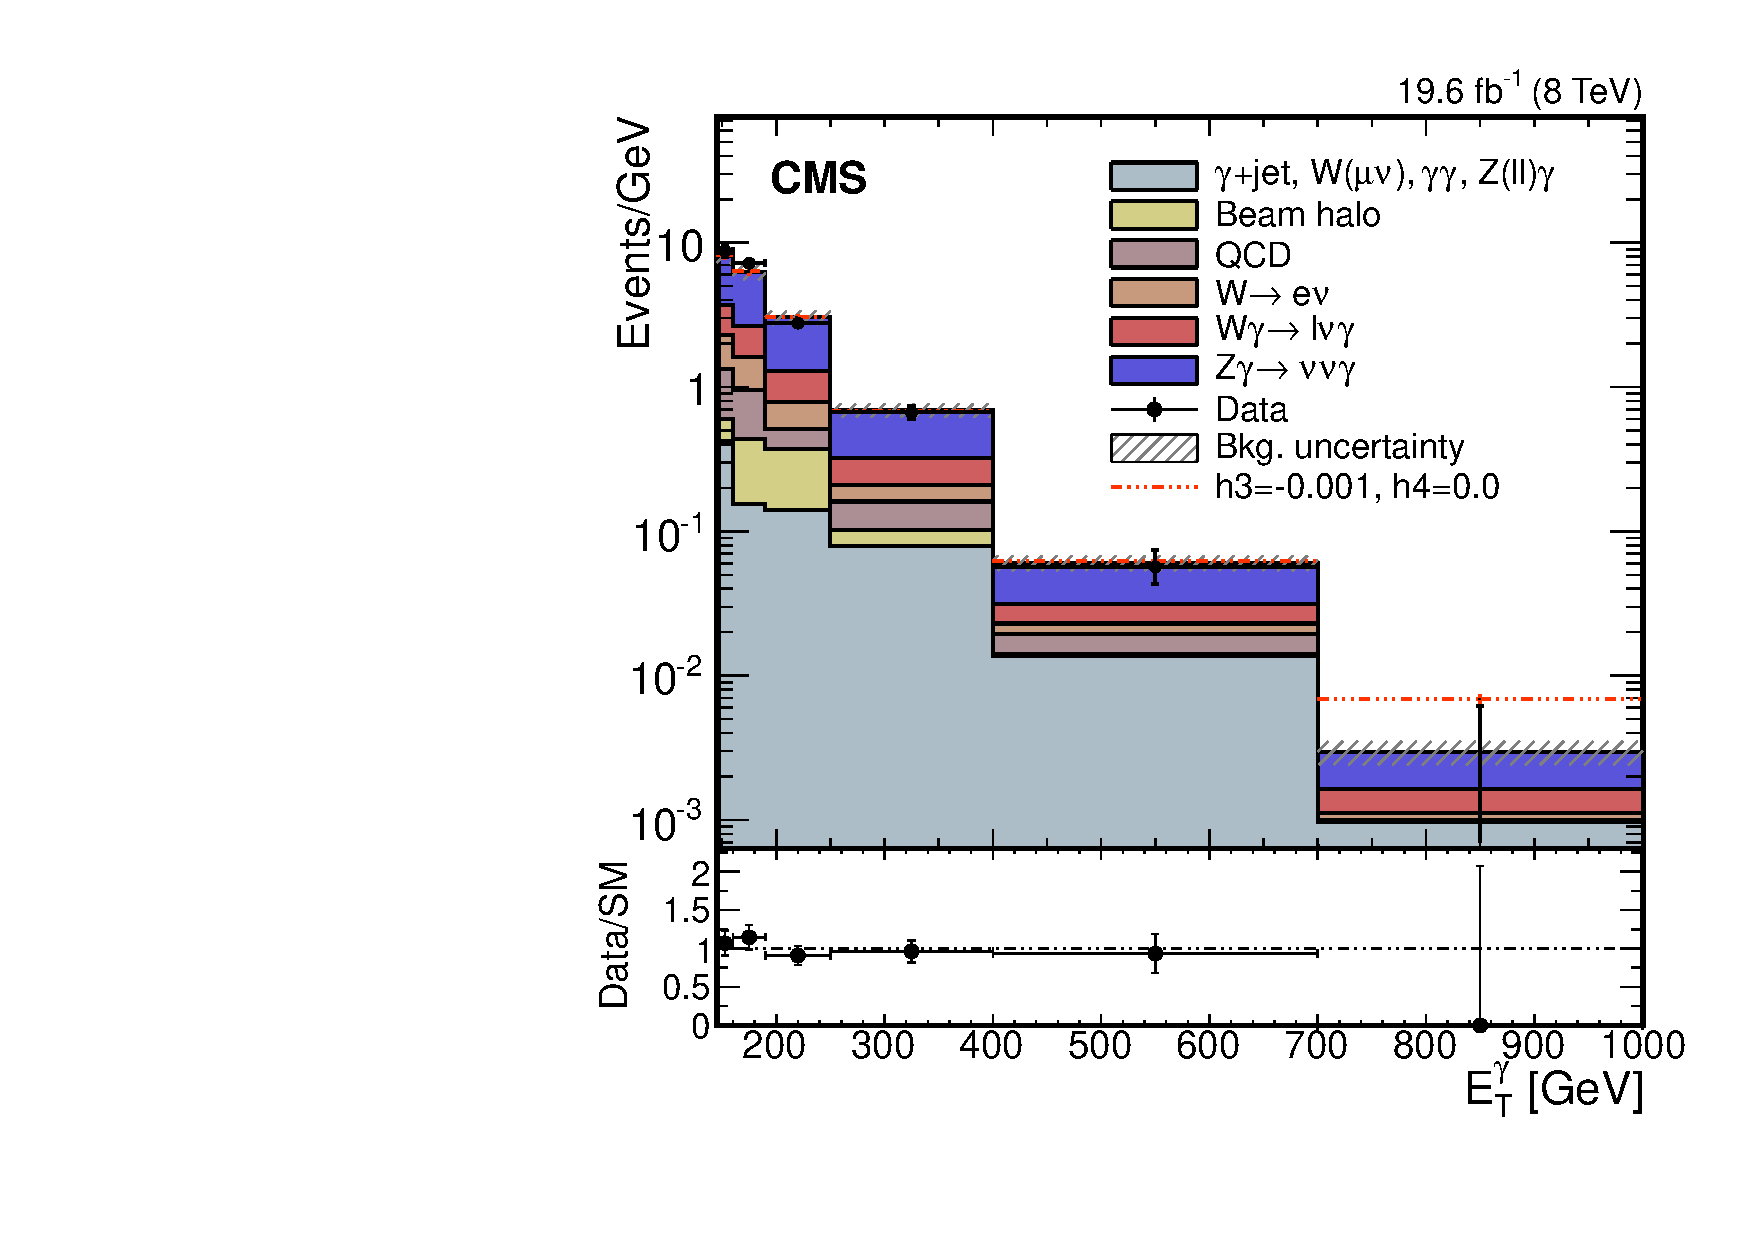
\includegraphics[width=0.45\textwidth]{figures/sss-inclboson-diboson-Vgamma-zgamvvgamptgam.pdf}
  \caption{ 
  The $\ET(\gamma)$ distribution from CMS~\cite{Khachatryan:2016yro} in data (points) compared to signal and estimated background contributions (histogram). A ATGC signal with $\hthreev=-0.001$ is 
  shown (dot-dashed histogram) for comparison. The background uncertainty includes statistical and systematic contributions. 
}
\label{fig:sss-inclboson-diboson-Vgamma-zgamvvgamptgam}
\end{center}
\end{figure}

The resulting 95\% CL limits for charged (\Wg) and neutral (\Zg) TGC are listed in Table~\ref{tab:sss-Vgamma-ATGC}. For comparison, only limits obtained without the use of a form factor are listed. ATLAS
also provides limits with unitarity-preserving form factors, and in case of the $\rts=8\TeV$  analysis limits as a function of the dipole form factor scale $\Lambda$~\cite{Aad:2016sau}. 

\begin{table}\centering
\resizebox{\textwidth}{!}{
\begin{tabular}{|c|c|c|c|c|c|c|c|}
& & & & \multicolumn{2}{c} {ATLAS} & CMS   \\ 
& Process & \rts\;[TeV] & $\mathcal{L} [\ifb]$ ATLAS, CMS & Observed & Expected & Observed  \\
\hline

$\dkg$&\Wglvg& 7 &$4.6,5$& $[-0.41, 0.46]$ & $[-0.38, 0.43]$ & $[-0.38, 0.29]$  \\
$\lg$&\Wglvg& 7 &$4.6,5$& $[-0.065, 0.061]$ & $[-0.060, 0.056]$ & $[-0.050, 0.037]$ \\
$\hthreeg$ &\Zgllg,\Zgvvg& 7 &$4.6,5.0$& $[-0.015, 0.016]$ & $[-0.017, 0.018]$ & $<2.9\cdot 10^{-3}$ \\
$\hthreez$ &\Zgllg,\Zgvvg& 7 &$4.6,5.0$& $[-0.013, 0.014]$ & $[-0.015, 0.016]$ & $<2.7 \cdot 10^{-3}$  \\
$\hfourg$ & \Zgllg,\Zgvvg & 7 &$4.6,5.0$& $[-9.4 \cdot 10^{-5}, 9.2 \cdot 10^{-5}]$ & $[-1.0 \cdot 10^{-4}, 1.0 \cdot 10^{4}]$ & $<1.5 \cdot 10^{-5}$  \\
$\hfourz$ & \Zgllg,\Zgvvg & 7 &$4.6,5.0$& $[-8.7 \cdot 10^{-5}, 8.7 \cdot 10^{-5}]$ & $[-9.7 \cdot 10^{-5}, 9.7 \cdot 10^{5}]$ & $<1.3 \cdot 10^{-5}$  \\
$\hthreeg$ &\Zgllg,\Zgvvg& 8 &$20.3, - $& $[-9.5\cdot 10^{-4}, 9.9\cdot 10^{-4}]$ & $[-1.8\cdot 10^{-3}, 1.8\cdot 10^{-3}]$ & -- \\
$\hthreez$ &\Zgllg,\Zgvvg& 8 &$20.3, - $& $[-7.8\cdot 10^{-4}, 8.6\cdot 10^{-4}]$ & $[-1.5\cdot 10^{-3}, 1.5\cdot 10^{-3}]$ & -- \\
$\hfourg$  &\Zgllg,\Zgvvg& 8 &$20.3, - $& $[-3.2\cdot 10^{-6}, 3.2\cdot 10^{-6}]$ & $[-6.0\cdot 10^{-6}, 5.9\cdot 10^{-6}]$ & -- \\
$\hfourz$  &\Zgllg,\Zgvvg& 8 &$20.3, - $& $[-3.0\cdot 10^{-6}, 2.9\cdot 10^{-6}]$ & $[-5.5\cdot 10^{-6}, 5.4\cdot 10^{-6}]$ & -- \\
$\hthreeg$ &\Zgllg& 8 &$-, 19.5$& -- & -- & $[-4.6 \cdot 10^{-3}, 4.6 \cdot 10^{-3}]$ \\
$\hthreez$ &\Zgllg& 8 &$-, 19.5$& -- & -- & $[-3.8 \cdot 10^{-3}, 3.7 \cdot 10^{-3}]$ \\
$\hfourg$ &\Zgllg& 8 &$-, 19.5$& -- & -- & $[-3.6 \cdot 10^{-5}, 3.5 \cdot 10^{-5}]$ \\
$\hfourz$ &\Zgllg& 8 &$-, 19.5$& -- & -- & $[-3.1 \cdot 10^{-5}, 3.0 \cdot 10^{-5}]$ \\
$\hthreeg$ &\Zgvvg& 8 &$-, 19.5$& -- & -- & $[-1.1 \cdot 10^{-3}, 0.9 \cdot 10^{-3}]$ \\
$\hthreez$ &\Zgvvg& 8 &$-, 19.5$& -- & -- & $[-1.5 \cdot 10^{-3}, 1.6 \cdot 10^{-3}]$ \\
$\hfourg$ &\Zgvvg& 8 &$-, 19.5$& -- & -- & $[-3.8 \cdot 10^{-6}, 4.3 \cdot 10^{-6}]$ \\
$\hfourz$ &\Zgvvg& 8 &$-, 19.5$& -- & -- & $[-3.9 \cdot 10^{-6}, 4.5 \cdot 10^{-6}]$ \\

\end{tabular}
}
\caption{Expected and observed 95\% CL on \hthreeg, \hthreez, \hfourg, and \hfourz\; measured in the 
\Zgllg\; and \Zgvvg\; final states from the ATLAS and CMS collaborations.}
\label{tab:sss-Vgamma-ATGC}
\end{table}







\subsection{Inclusive tri-boson production}

One avenue for testing quartic gauge boson interactions is through
inclusive tri-boson production: $pp\ to VV^{\prime}V^{\prime\prime}$
for $V= \gamma, W, Z$.  Using the Run 1 data sample, the triply heavy
such channels ($WWW, WWZ, WZZ, ZZZ$) are not accessible anywhere near
SM rates, due to their small 8 TeV cross sections and large
multi-lepton backgrounds. The photonic channels do not suffer as much
from these problems, and sensitivity is at or near SM rates in Run 1. 

ATLAS $W\gamma\gamma$~\cite{Aad:2015uqa}
\begin{figure}[p]
    \centering
    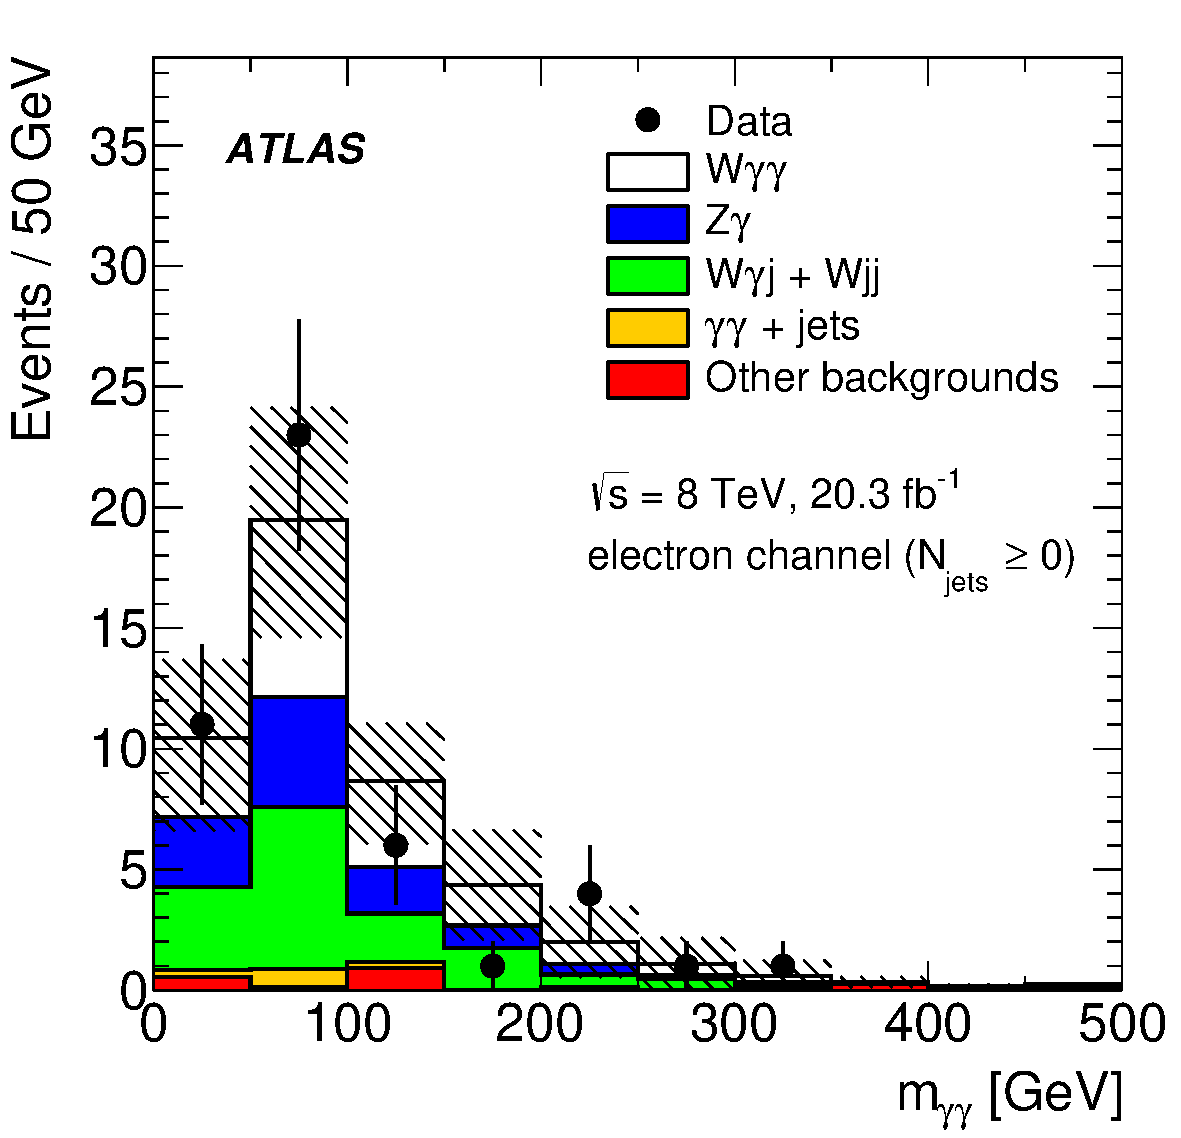
\includegraphics[width=0.45\textwidth]{figures/ss-inclboson-triboson-wgg-ele-atlas8tev.pdf}
    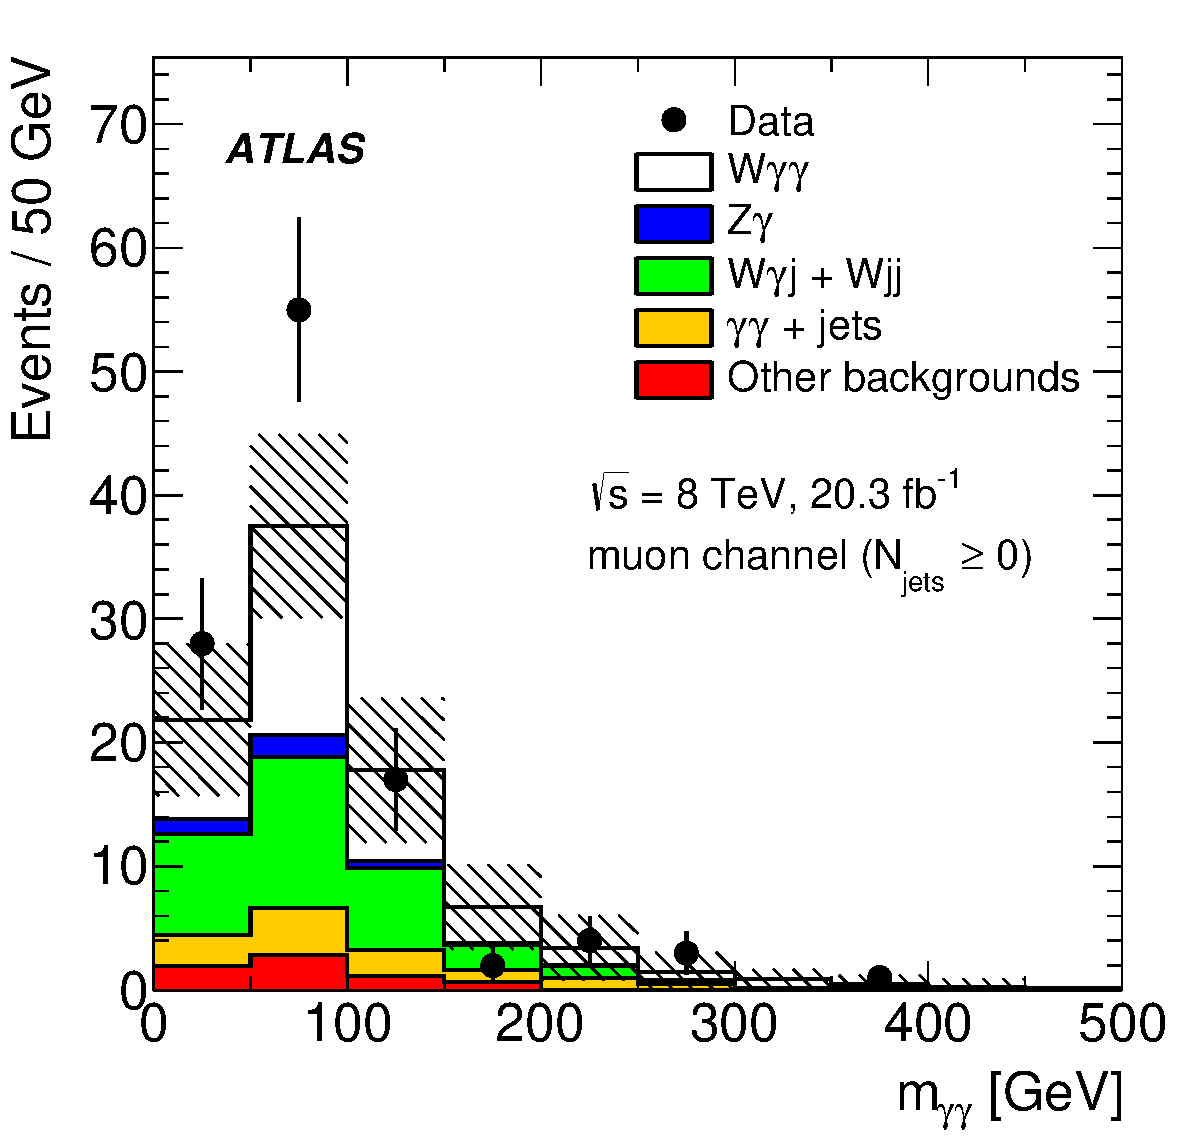
\includegraphics[width=0.45\textwidth]{figures/ss-inclboson-triboson-wgg-mu-atlas8tev.pdf}
    \caption{}
    \label{fig:ss-inclboson-triboson-wgg-atlas8tev}
\end{figure}


CMS WVgamma 8 \TeV~\cite{Chatrchyan:2014bza}

\begin{figure}[p]
    \centering
    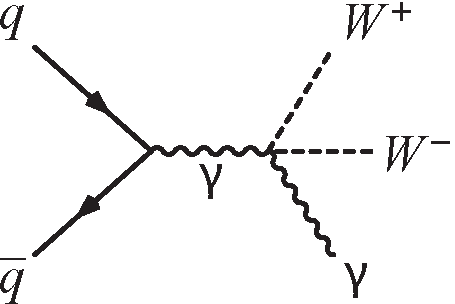
\includegraphics[width=0.45\textwidth]{figures/ss-inclboson-triboson-wvg-diagram1.pdf}
    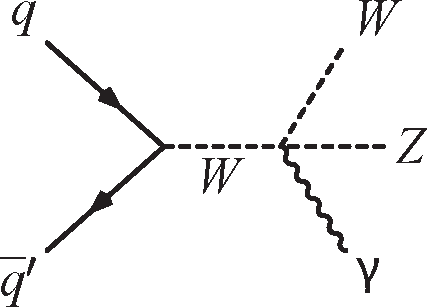
\includegraphics[width=0.45\textwidth]{figures/ss-inclboson-triboson-wvg-diagram2.pdf}
    \caption{}
    \label{fig:ss-inclboson-triboson-wvg-diagrams}
\end{figure}
\begin{figure}[p]
    \centering
    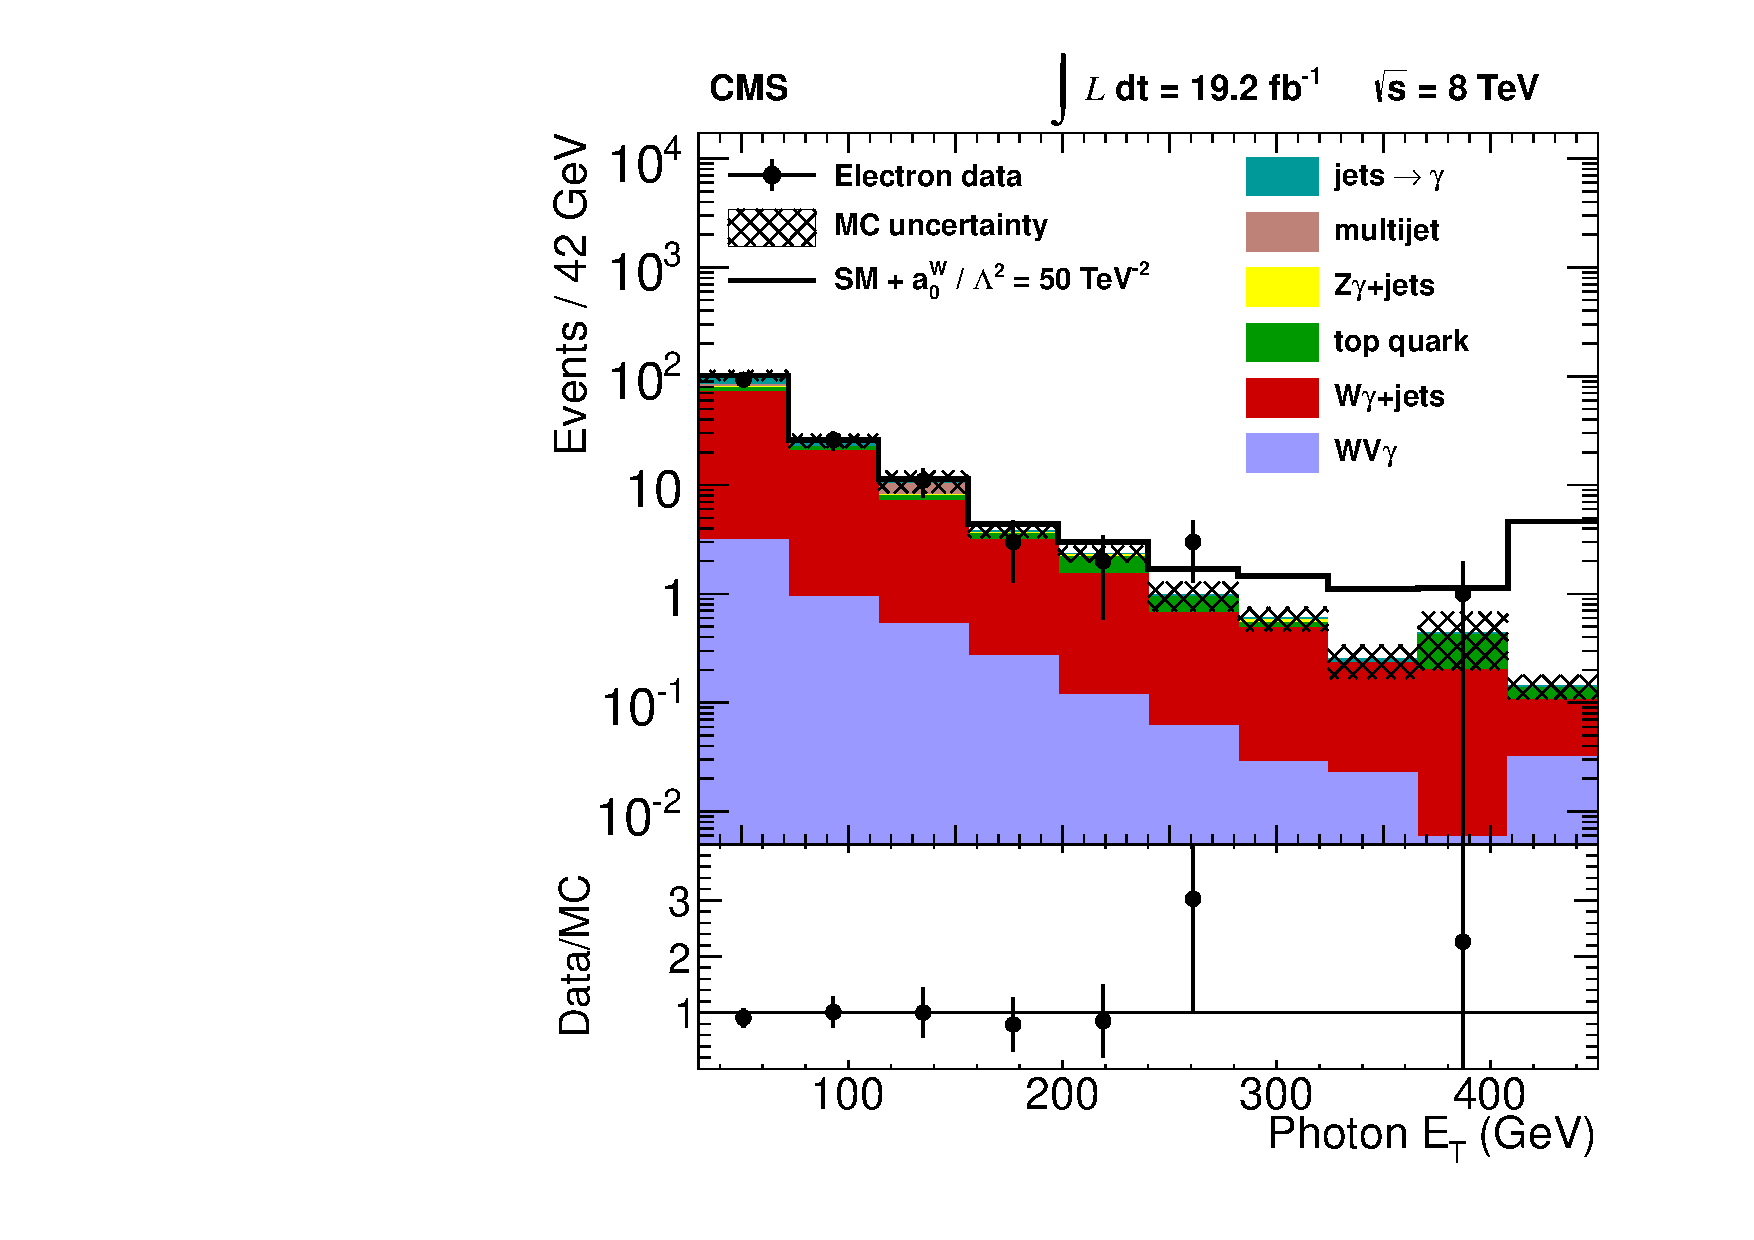
\includegraphics[width=0.45\textwidth]{figures/ss-inclboson-triboson-wvg-ele-cms8tev.pdf}
    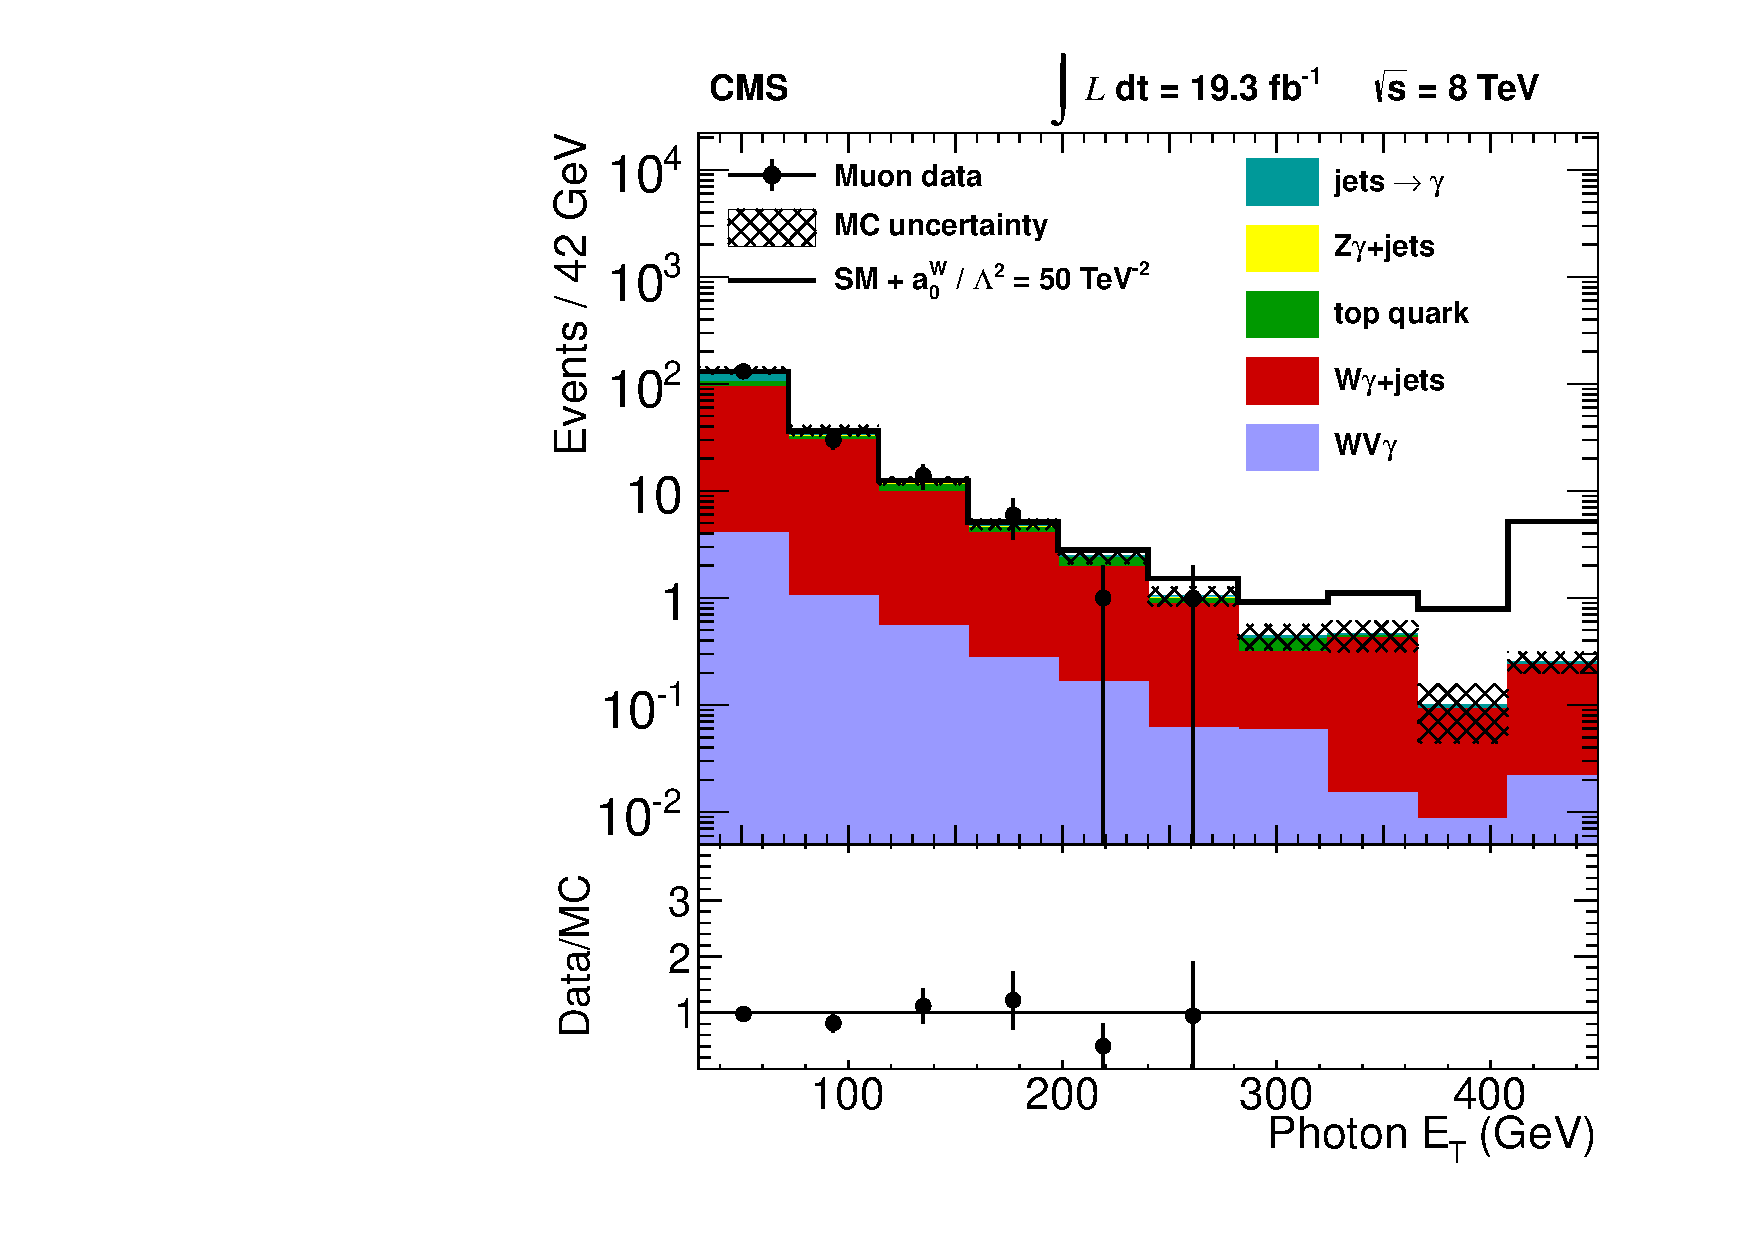
\includegraphics[width=0.45\textwidth]{figures/ss-inclboson-triboson-wvg-mu-cms8tev.pdf}
    \caption{}
    \label{fig:ss-inclboson-triboson-wvg-cms8tev}
\end{figure}


\section{Exclusive boson production}
\subsection{Exclusive single boson production, vector-boson fusion}
\begin{figure}[p]
    \centering
    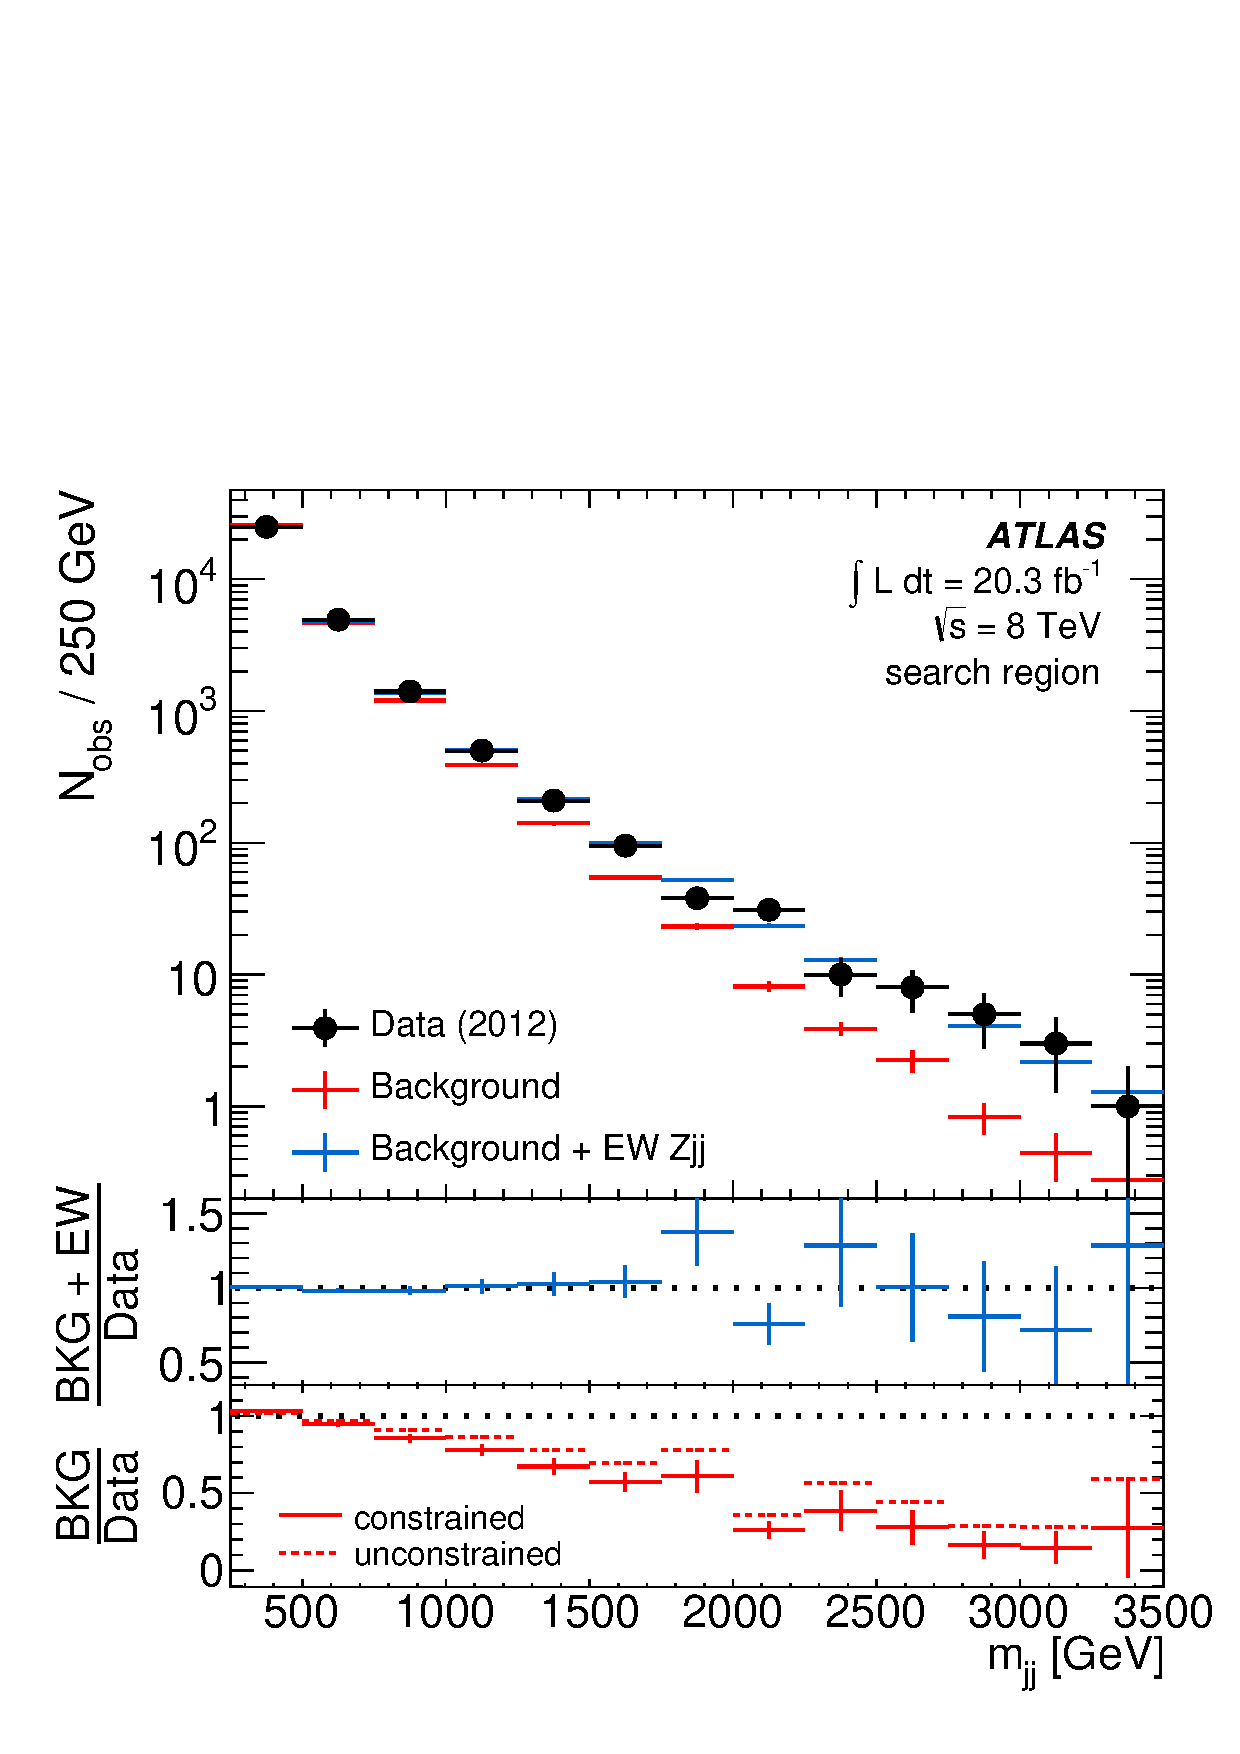
\includegraphics[height=0.3\textheight]{figures/ss-exclboson-z2j-atlas8tev}
    \caption{}
    \label{fig:ss-exclboson-z2j-atlas8tev}
\end{figure}
ATLAS VBF Z 7 \TeV~\cite{Aad:2014dta}

CMS VBF Z 7 \TeV~\cite{Chatrchyan:2013jya}

CMS VBF Z 8 \TeV~\cite{Khachatryan:2014dea}


\subsection{Exclusive di-boson production, vector-boson scattering}
%\begin{figure}[p]
%    \centering
%    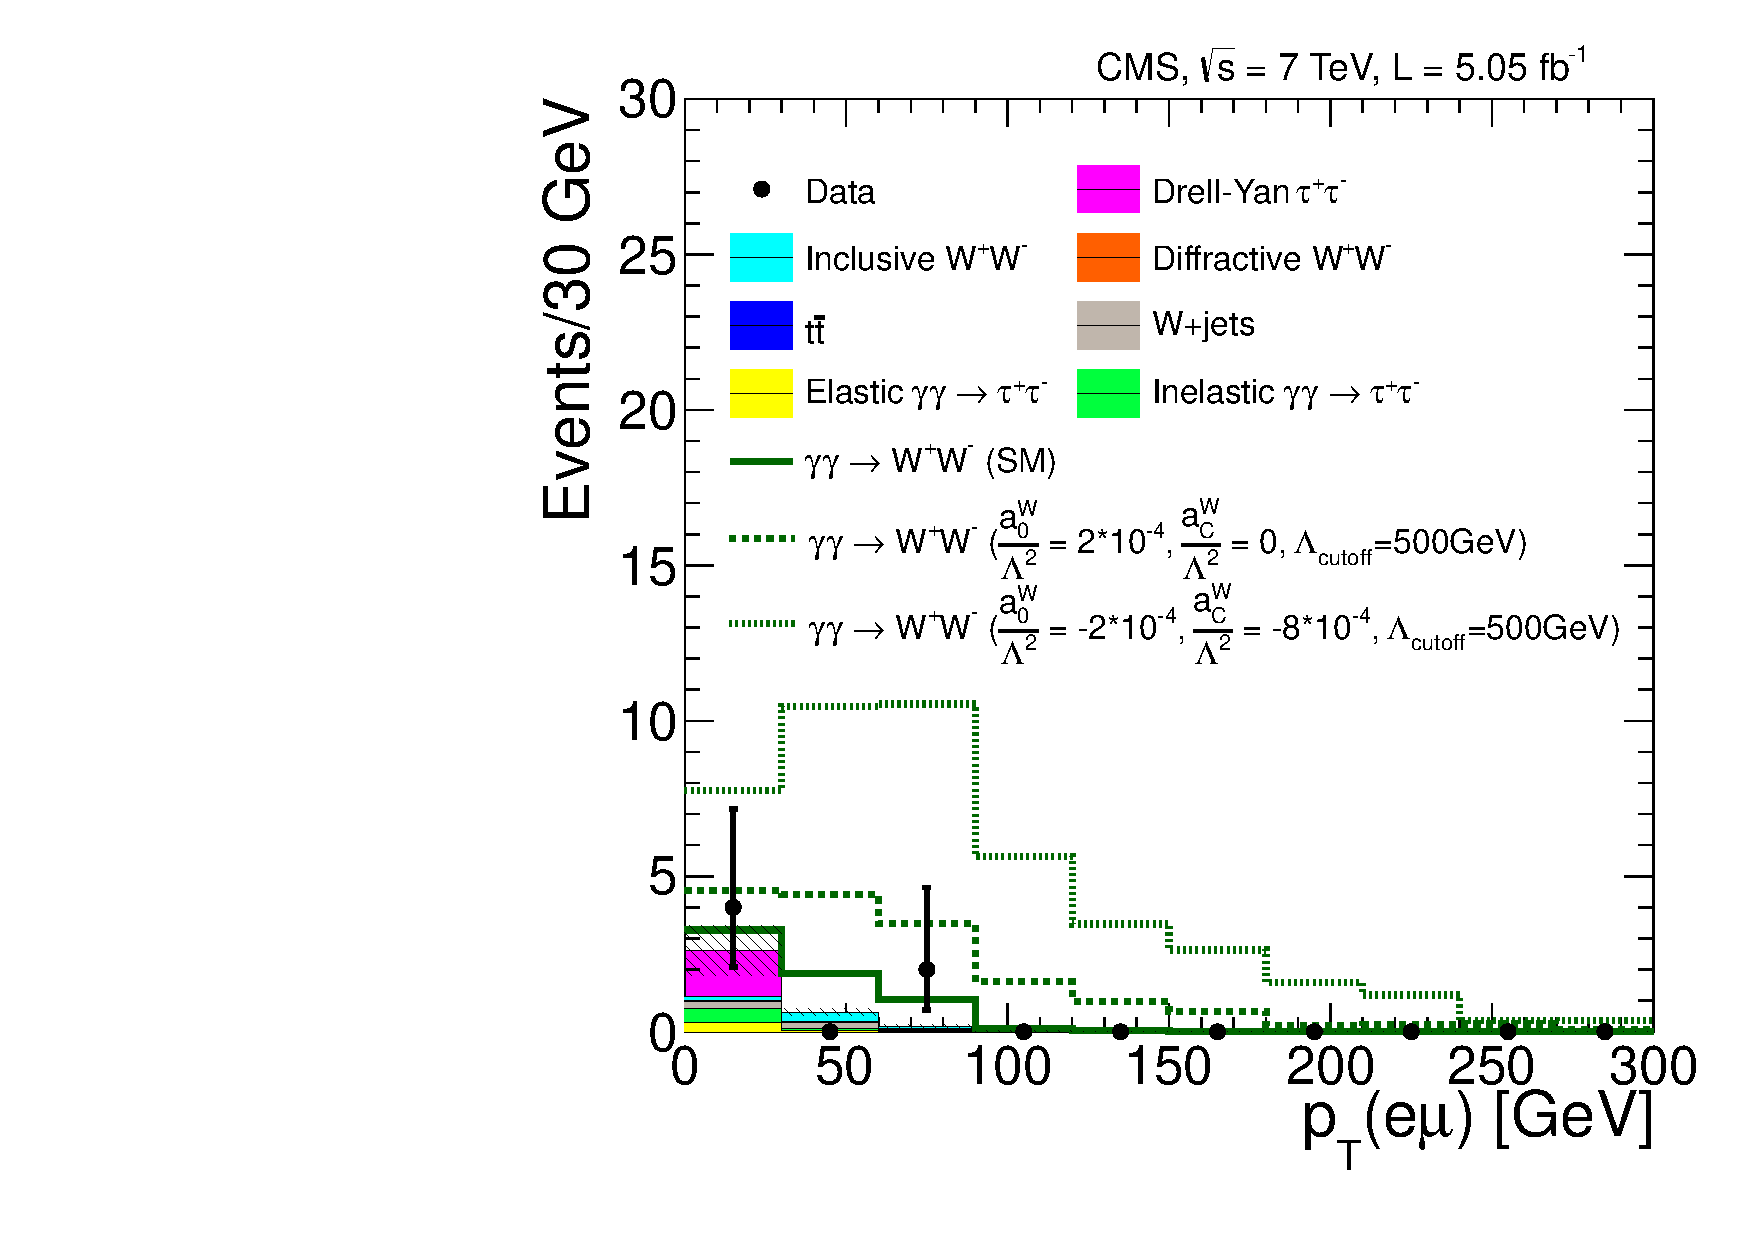
\includegraphics[height=0.3\textheight]{figures/ss-exclboson-ww-cms7tev}
%    \caption{}
%    \label{fig:ss-exclboson-ww-cms7tev}
%\end{figure}
%CMS WWexcl 7 \TeV~\cite{Chatrchyan:2013foa}

In addition to exclusive single boson production, CMS and ATLAS have
evidence for exclusive diboson production, in two different channels.
In one of them, CMS~\cite{Khachatryan:2016mud} has performed a search
for exclusive diboson production via protons emitting (possibly
quasi-) real photons which rescatter to produce $W^+W^-$ pairs:
$pp \to p^{(*)}W^+ W^- p^{(*)} \to p^{(*)}\mu^{\pm}e^{\mp}p^{(*)}$,
where $p^*$ admits the possibility that the protons dissociate into an
undetected system.  Such production is characterized by a
$\mu^{\pm}e^{\mp}$ pair which has no underlying event activity typical
of proton-proton hard scattering.  By selecting a $\mu^{\pm}e^{\mp}$
pair of sufficiently high individual (20 GeV) and joint (30 GeV)
transverse momentum, and requiring further that the two lepton tracks
intersect with each other, but have no additional tracks nearby, an
exclusive production signal is isolated from backgrounds such as
exclusive Drell-Yan and inclusive dilepton production from various
hard scattering mechanisms, respectively.  Selection efficiency is
validated by examining a control sample of exclusive same-flavor
Drell-Yan production ($p^{(*)}\mu^{\pm}\mu^{\mp}p^{(*)}$ or
$p^{(*)}e^{\pm}e^{\mp}p^{(*)}$) and comparing it with simulated
efficiency.  The relative contribution of dissociated proton
scattering for signal is also deduced by comparing the observed
exclusive Drell-Yan cross section with an exclusive matrix element
calculation (\texttt{LPAIR}~\cite{Vermaseren:1982cz,Baranov:1991yq});
proton dissociation is estimated to enhance the signal by a factor of
$4.10 \pm 0.43$ with respect to an exclusive calculation
from \texttt{MadGraph}.

Figure~\ref{fig:ss-exclboson-ww-cms8tev} shows the distributions of
dilepton $\pt$ and extra tracks in data compared with expectations
from simulation.  13 events are observed with an expected background
of $3.9\pm0.6$ in the 8 TeV data.  In the 7
TeV~\cite{Chatrchyan:2013foa} and 8 TeV data combined, a 3.4 $\sigma$
excess is observed over background as evidence for exclusive (plus
dissociative) $W^+W^-$ production.  The signal corresponds to a cross
section in the 8 TeV data of $11.9^{+5.6}_{-4.5}$ fb, in agreement
with a SM prediction of $6.9\pm0.6$ fb.  Exclusive $W^+W^-$ production
is sensitive to $WW\gamma\gamma$ quartic couplings. The CMS analysis
derived limits on the dimension 6 couplings $a^W_0/\Lambda^2$ and
$a^W_C/\Lambda^2$ and, in the context of dimension 8 EFT, the
anomalous couplings $f_{M(0,1,2,3)}/\Lambda^4$.  The 95\% CL upper
limits are $1.1(4.4)\times 10^{-4} \rm{GeV}^{-2}$ for
$a^W_0/\Lambda^2$ ($a^W_C/\Lambda^2$), and range from $2-17 \times
10^{-4} \rm{GeV}^{-4}$ for dimension 8 couplings, for models with no
form factor.  This process is the single best constraint on
$WW\gamma\gamma$ QGCs.

\begin{figure}[htb]
\centering
%\includegraphics[width=.48\textwidth]{Figures/2016_01_29_UpdatedPlots/ee_pt.pdf}
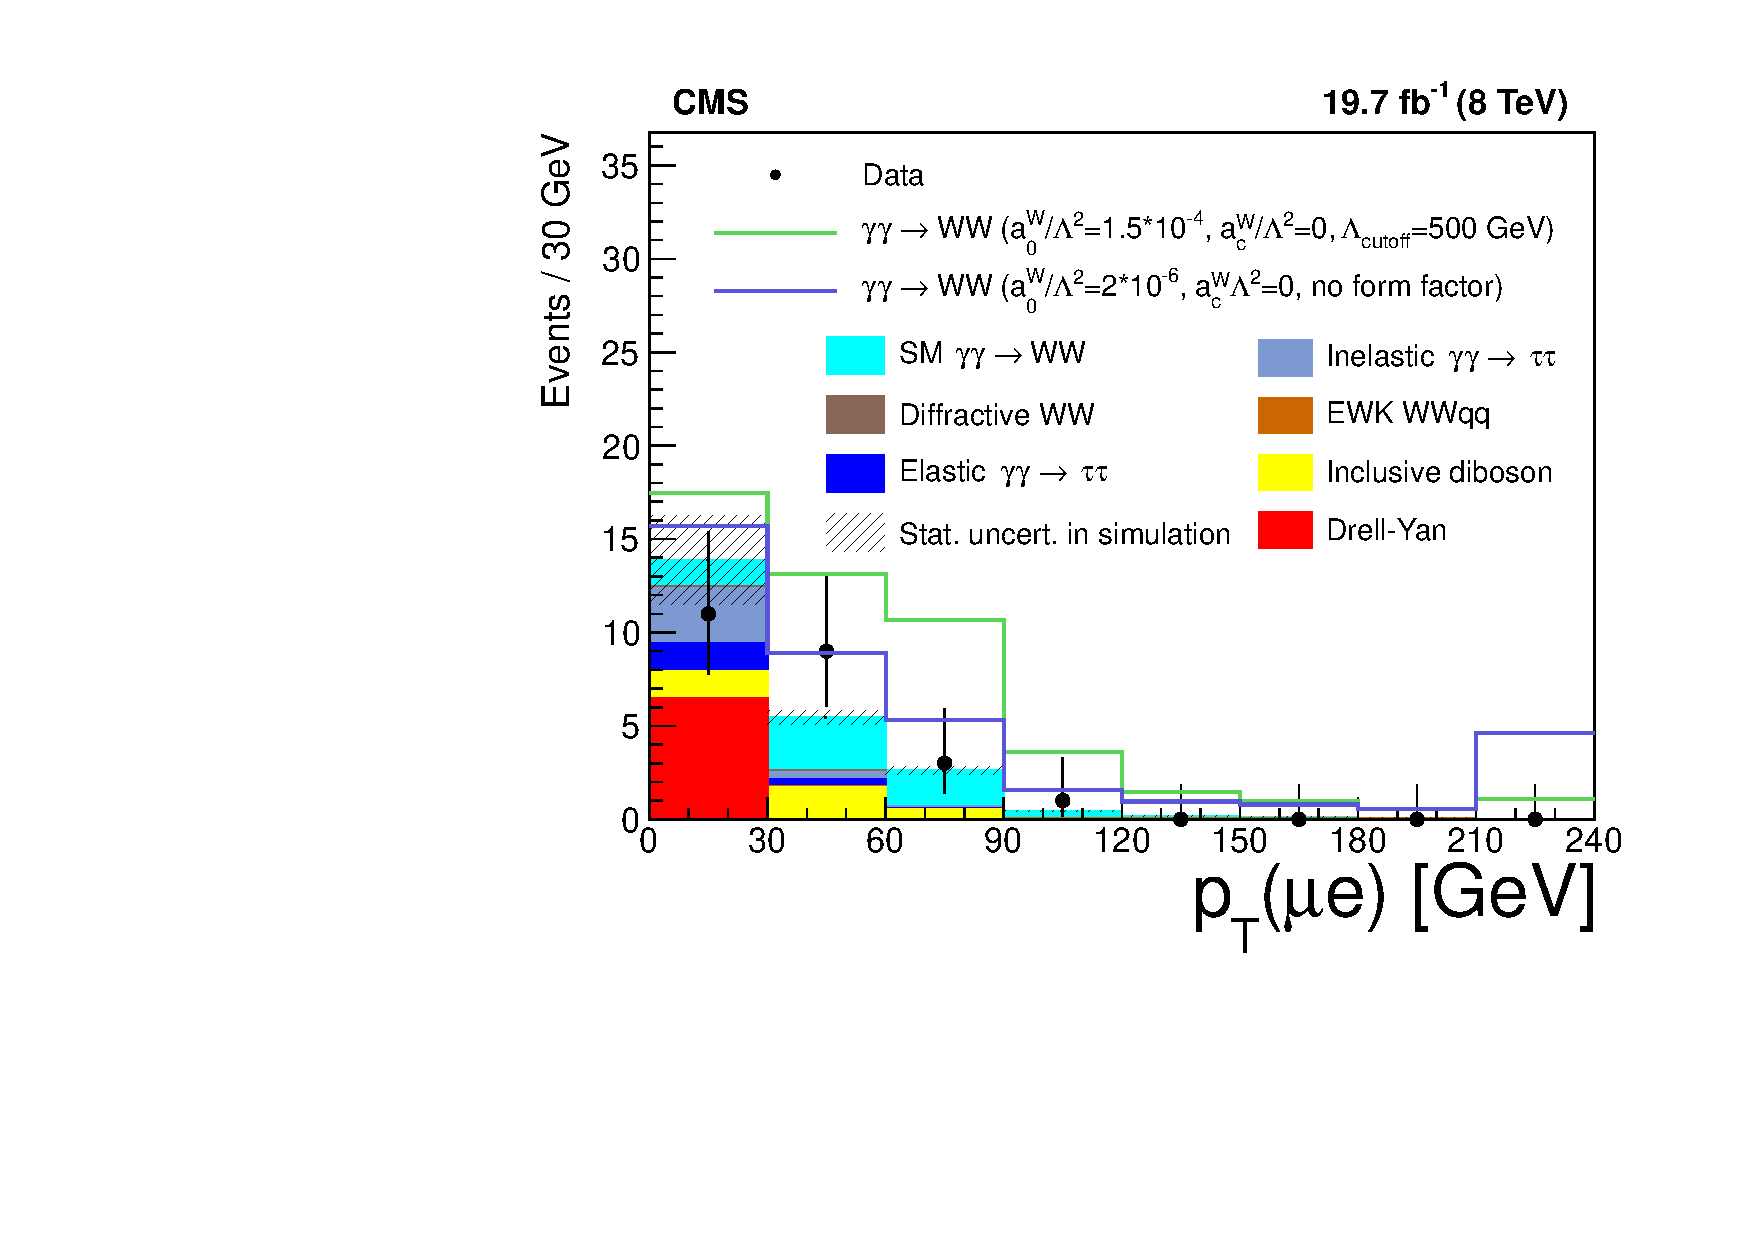
\includegraphics[width=.48\textwidth]{figures/ss-exclboson-ww-cms8tev-1.pdf}
%\includegraphics[width=.48\textwidth]{Figures/2016_01_29_UpdatedPlots/ee_tracks_
%pt30.pdf}
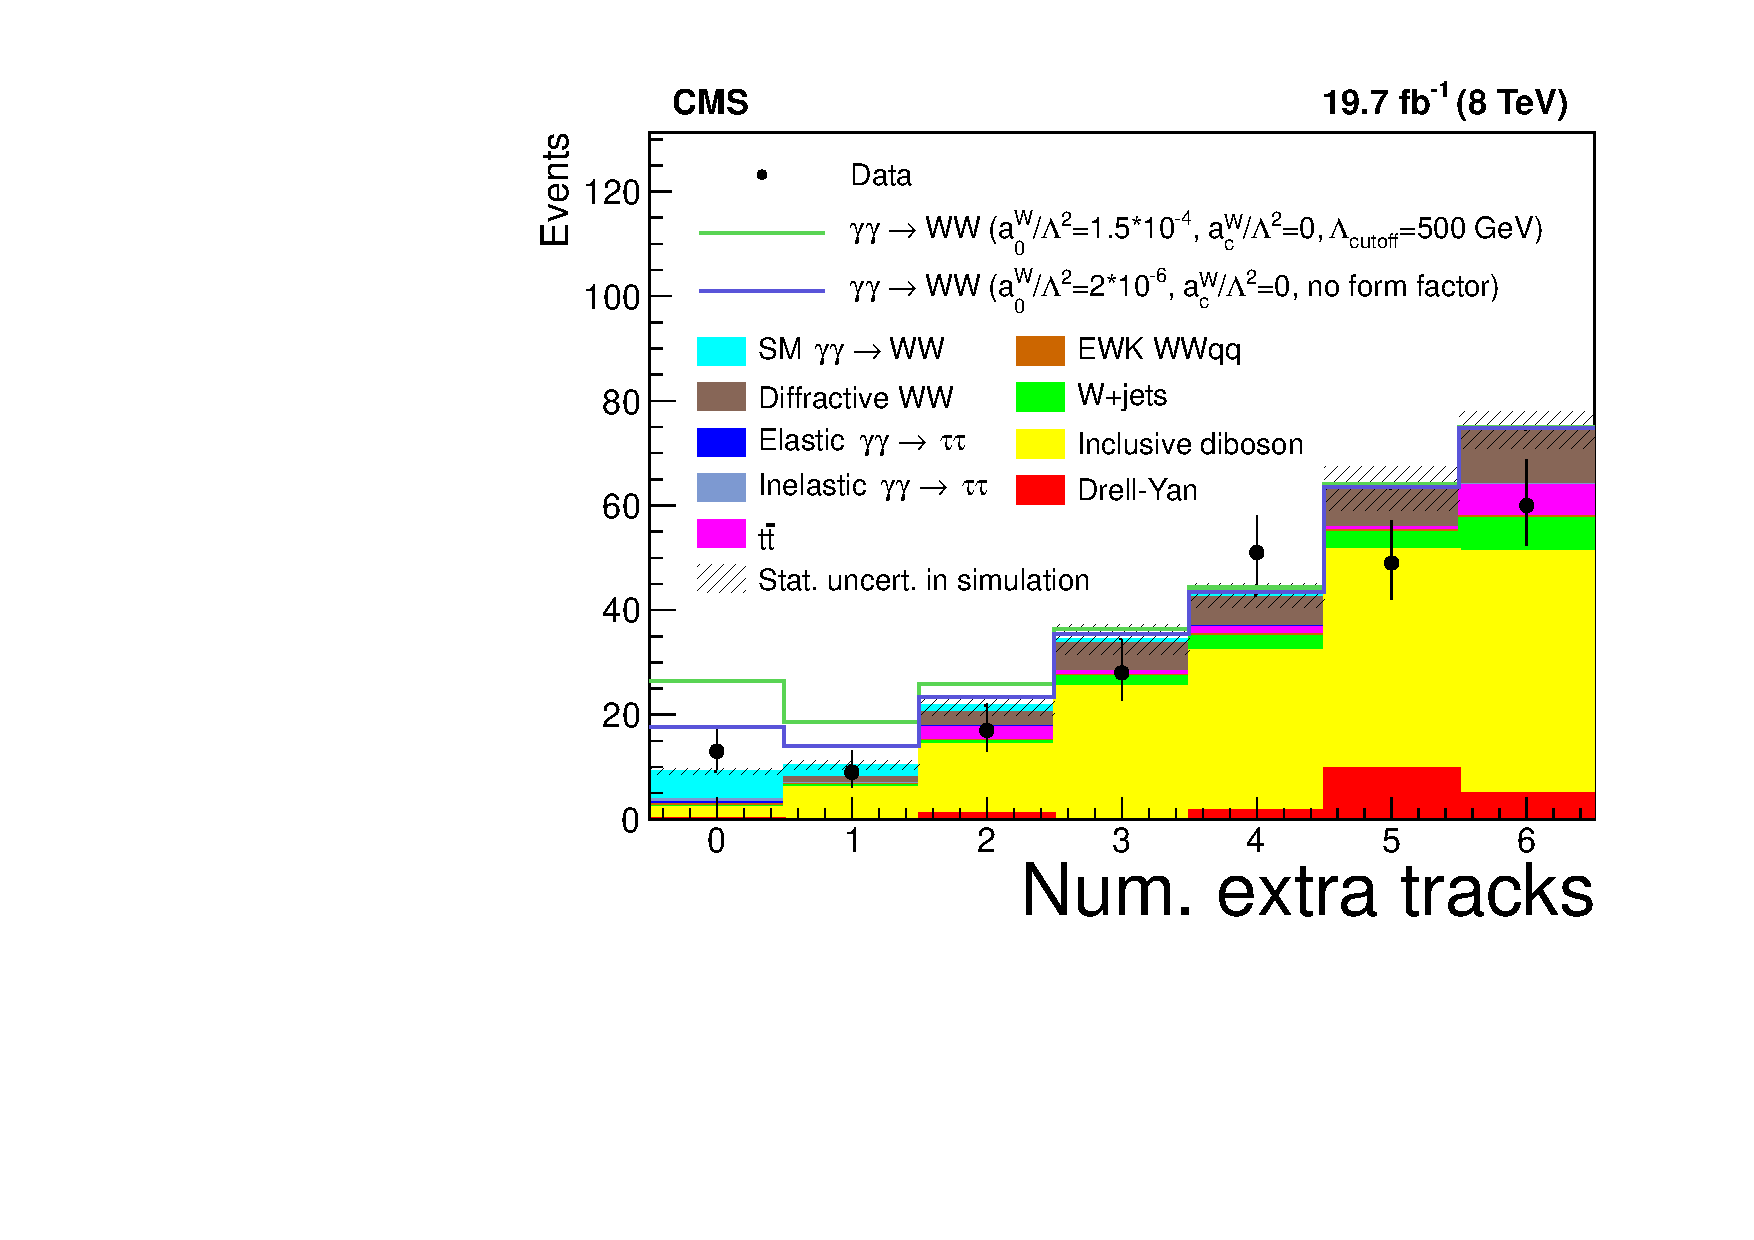
\includegraphics[width=.48\textwidth]{figures/ss-exclboson-ww-cms8tev-2.pdf}
\caption{Evidence for exclusive diboson production via $pp \to p^{(*)}W^+ W^- p^{(*)} \to p^{(*)}\mu^{\pm}e^{\mp}p^{(*)}$~\cite{Khachatryan:2016mud}.
Distributions of muon-electron transverse momentum for events with zero
 associated tracks (left), and extra-tracks multiplicity for events with $\pt(\mu^{\pm}e^{\mp}) > 30$ GeV (right).
 The data are shown by the points with error bars; the histograms indicate the expected SM signal and backgrounds.
\label{fig:ss-exclboson-ww-cms8tev}}
\end{figure}

The other exclusive diboson process for which the LHC has evidence is
same-sign $WW$ production, via the process $qq \to WW +
2q \to \ell^\pm\ell^\pm + 2 \rm{jet} + \met$.  Similar to exclusive
single boson production, the final state of interest is a
superposition of several amplitudes at leading order, some of which
are purely electroweak and include triple and quartic gauge boson
interactions (see Fig.~\ref{fig:ss-exclboson-ww-sigdiagram}), and
some of which have the final state jets arise from QCD initial- and
final-state radiation. Through a suitable choice of final state phase
space, the electroweak amplitudes are enhanced and the associated
signal strength and distributions can be tested against the
electroweak theory.  The same-sign $WW$ final state has the advantage
over other exclusive diboson channels ($\WW$ or $\WZ$) of a smaller
relative QCD amplitude and smaller multi-lepton backgrounds from top
quark, Drell-Yan, and $\WZ$ processes due to the same-sign dilepton
requirement.

An ATLAS analysis~\cite{Aad:2014zda} selects an ``inclusive region''
which is an admixture of electroweak and QCD contributions, and a VBS
signal region which is predominantly electroweak.  The inclusive
region requires two same-sign leptons with $\pt > 25$ GeV, $\met > 40$
GeV, and at least two jets with $m_{jj} > 500$ GeV for the two highest
$\pt$ jets; the VBS region further requires that the two highest $\pt$
jets are separated in rapidity, $|\Delta y_{jj}| > 2.4$.  To reduce
Drell-Yan background, events with dilepton mass less than 20 GeV or
dielectrons within 10 GeV of the $\Zzero$ mass are vetoed.  Top quark
background is reduced by vetoing events with b-tagged jets. Finally,
$WZ$ background is reduced by vetoing events with a third lepton with
muon $\pt > 6$ GeV or electron $\pt > 7$ GeV.  This results in 50
events selected for the inclusive region (as shown in
Fig.~\ref{fig:ss-exclboson-ww-ss}) and 34 for the VBS region.  About
half of selected events in either region are backgrounds from $\WZ$,
$W\gamma$ with photon conversion, and misidentified leptons from jets
in $V$ + jet processes.  The significance of the signal in the
inclusive region is observed (expected) to be 4.5$\sigma$
(3.4$\sigma$), and for the VBS region the significance is observed
(expected) to be 3.6$\sigma$ (2.8$\sigma$).  The measured cross
sections in these two regions are $2.1\pm 0.5\rm{(stat)} \pm
0.3\rm{(syst)}$ fb and $1.3 \pm 0.4\rm{(stat)}\pm 0.2\rm{(syst)}$ fb,
comparing well with SM predictions
from \texttt{Powheg-Box}~\cite{Nason:2004rx,Frixione:2007vw,Alioli:2010xd,Jager:2009xx,Melia:2010bm,Melia:2011gk}
of $1.52 \pm 0.11$ fb and $0.95\pm 0.06$ fb, respectively.

The VBS cross section is used to constrain parameters of an effective
chiral Lagrangian theory of vector boson
scattering~\cite{Alboteanu:2008my}, calculated
by \texttt{Whizard}~\cite{Kilian:2007gr,Moretti:2001zz}: $−0.14
< \alpha_4 < 0.16$ and $−0.23 < \alpha_5 < 0.24$ limits are obtained
at 95\% CL.

A CMS analysis~\cite{Khachatryan:2014sta} selects events similar to
the ATLAS VBS region: two same-sign leptons with $\pt>20$ GeV, two
jets with $m_{jj}>500$ GeV and $|\Delta \eta_{jj}| > 2.5$, and $\met >
40$ GeV.  There is a same-flavor Drell-Yan veto for events with
dilepton mass less than 50 GeV or dielectrons within 15 GeV of the Z
mass, a veto of top-like events with secondary vertex or soft muon
tags, and a third lepton veto for $\pt > 10$ GeV.  The 12 events so
selected are shown in Fig.~\ref{fig:ss-exclboson-ww-ss}.  About half
of them are expected to be background, mostly from misidentified
leptons. The resulting excess has a significance of 1.9$\sigma$
(2.9$\sigma$) observed (expected) for the purely electroweak
amplitude.  The observed fiducial cross section is
$4.0^{+2.4}_{−2.0} \rm{(stat)} ^{+1.1}_{−1.0} \rm{(syst)}$ fb compared
to an expected cross section estimated from \texttt{VBFNLO}~\cite{Baglio:2014uba,Arnold:2011wj,Arnold:2008rz} of
$5.8 \pm 1.2$ fb.

The $m_{\ell\ell}$ distribution of selected events is used to obtain
95\% CL bounds on dimension 8 EFT couplings $f_{S,(0,1)}$,
$f_{M,(0,1,6,7)}$, and $f_{T,(0,1,2)}$~\cite{Eboli:2006wa}.  For
$f_{S,(0,1)}$, which can correspond to a spin-one VBS resonance, the
limits are $-42 \rm{TeV}^{-4} < f_{S,0}/\Lambda^4 < 43 \rm{TeV}^{-4}$
and $-129 \rm{TeV}^{-4} < f_{S,1}/\Lambda^4 < 131 \rm{TeV}^{-4}$.

\begin{figure*}[htb] {
\centering
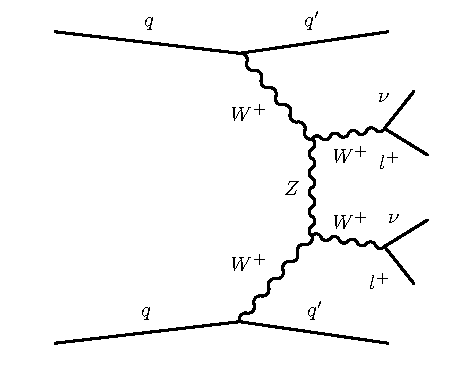
\includegraphics[width=0.315\textwidth]{figures/ss-exclboson-ww-diagram1.pdf}
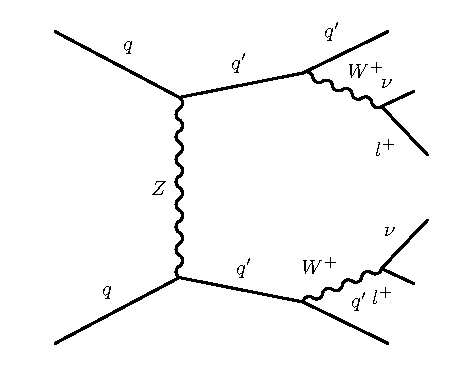
\includegraphics[width=0.35\textwidth]{figures/ss-exclboson-ww-diagram2.pdf}
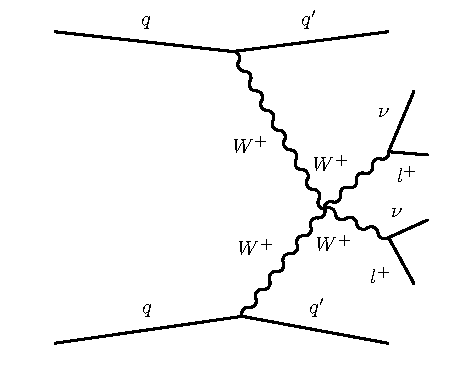
\includegraphics[width=0.315\textwidth]{figures/ss-exclboson-ww-diagram3.pdf}
\caption{
Representative Feynman diagrams for same-sign $WW$ production in association
with two jets from purely electroweak contributions:
(left) vector boson fusion,
(middle) bremsstrahlung-like,
and (right) multiperipheral production~\cite{Khachatryan:2014sta}.
\label{fig:ss-exclboson-ww-sigdiagram}}

}
\end{figure*}


\begin{figure}[p]
    \centering
    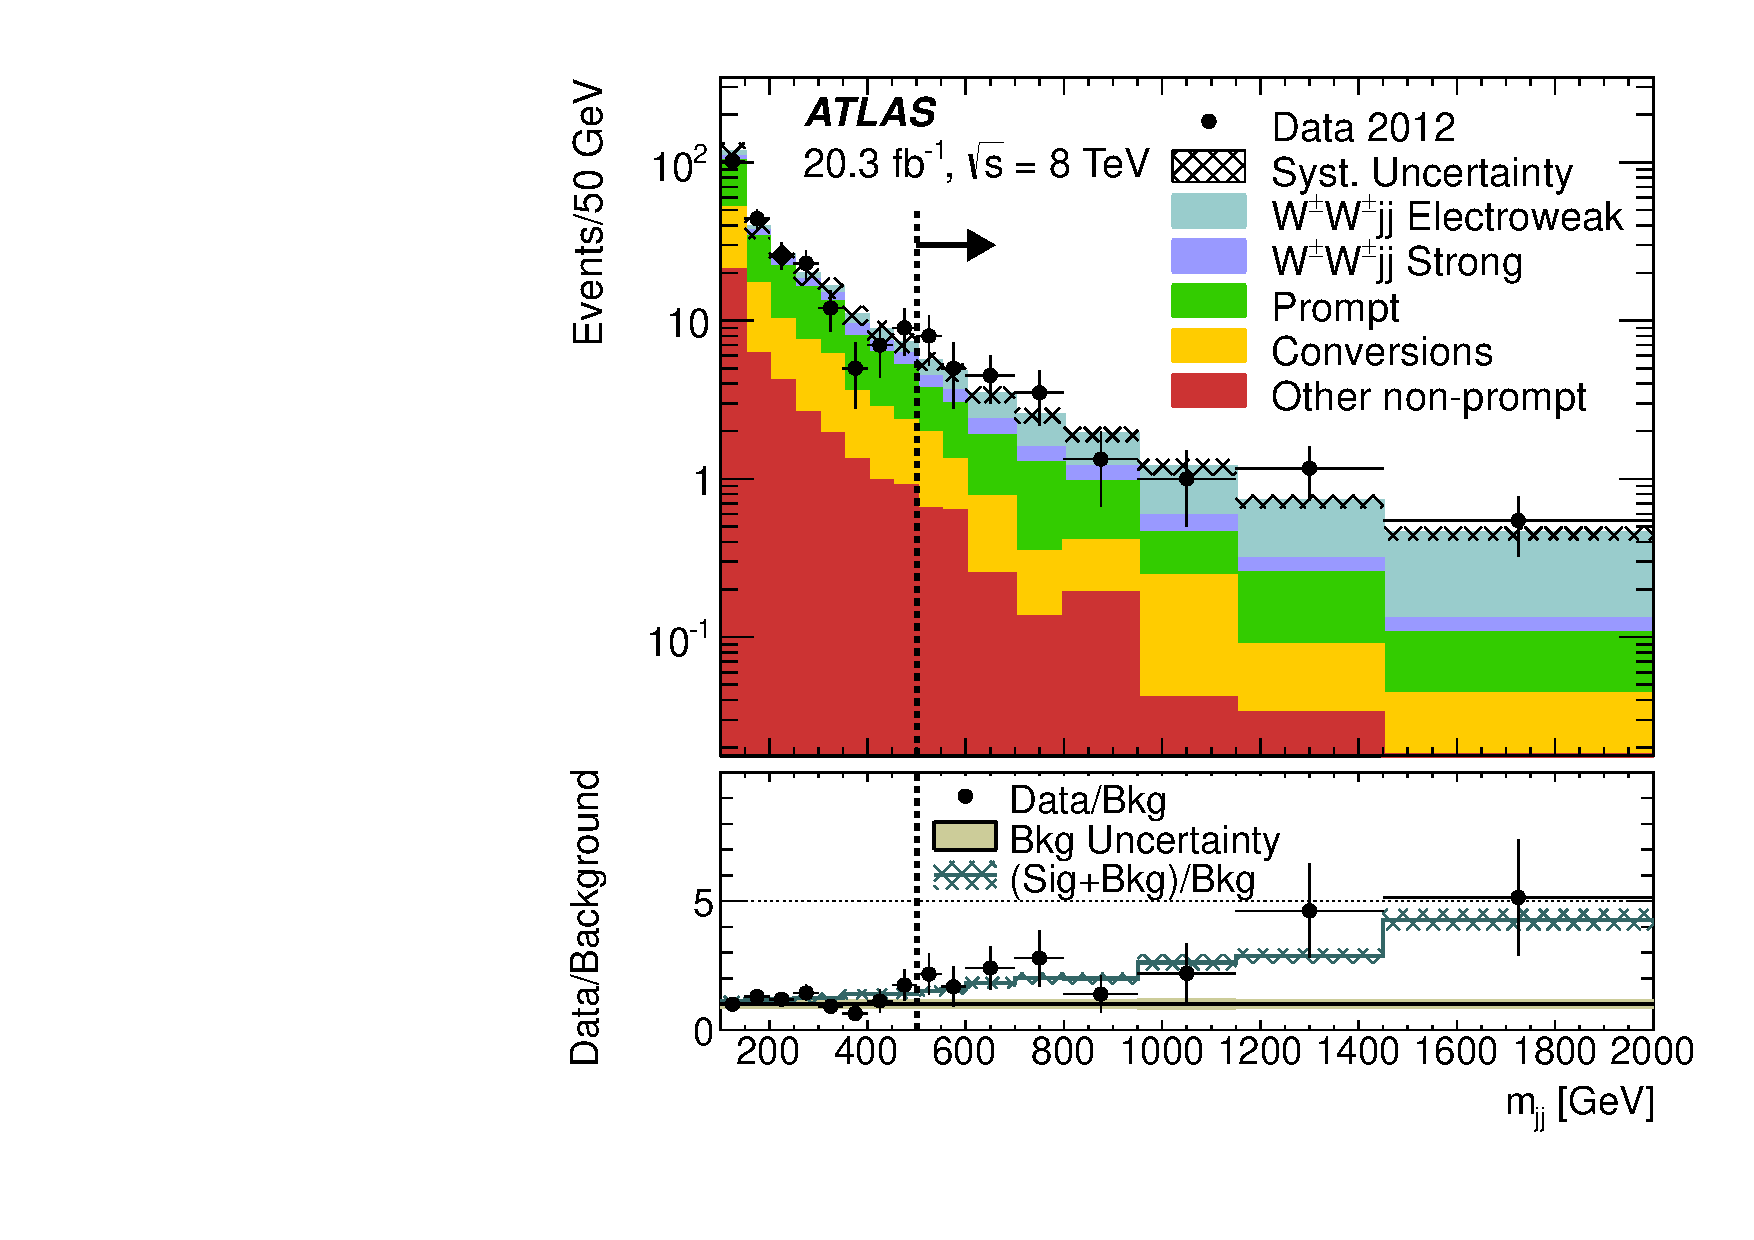
\includegraphics[width=0.45\textwidth]{figures/ss-exclboson-ww-ss-atlas8tev.pdf}
    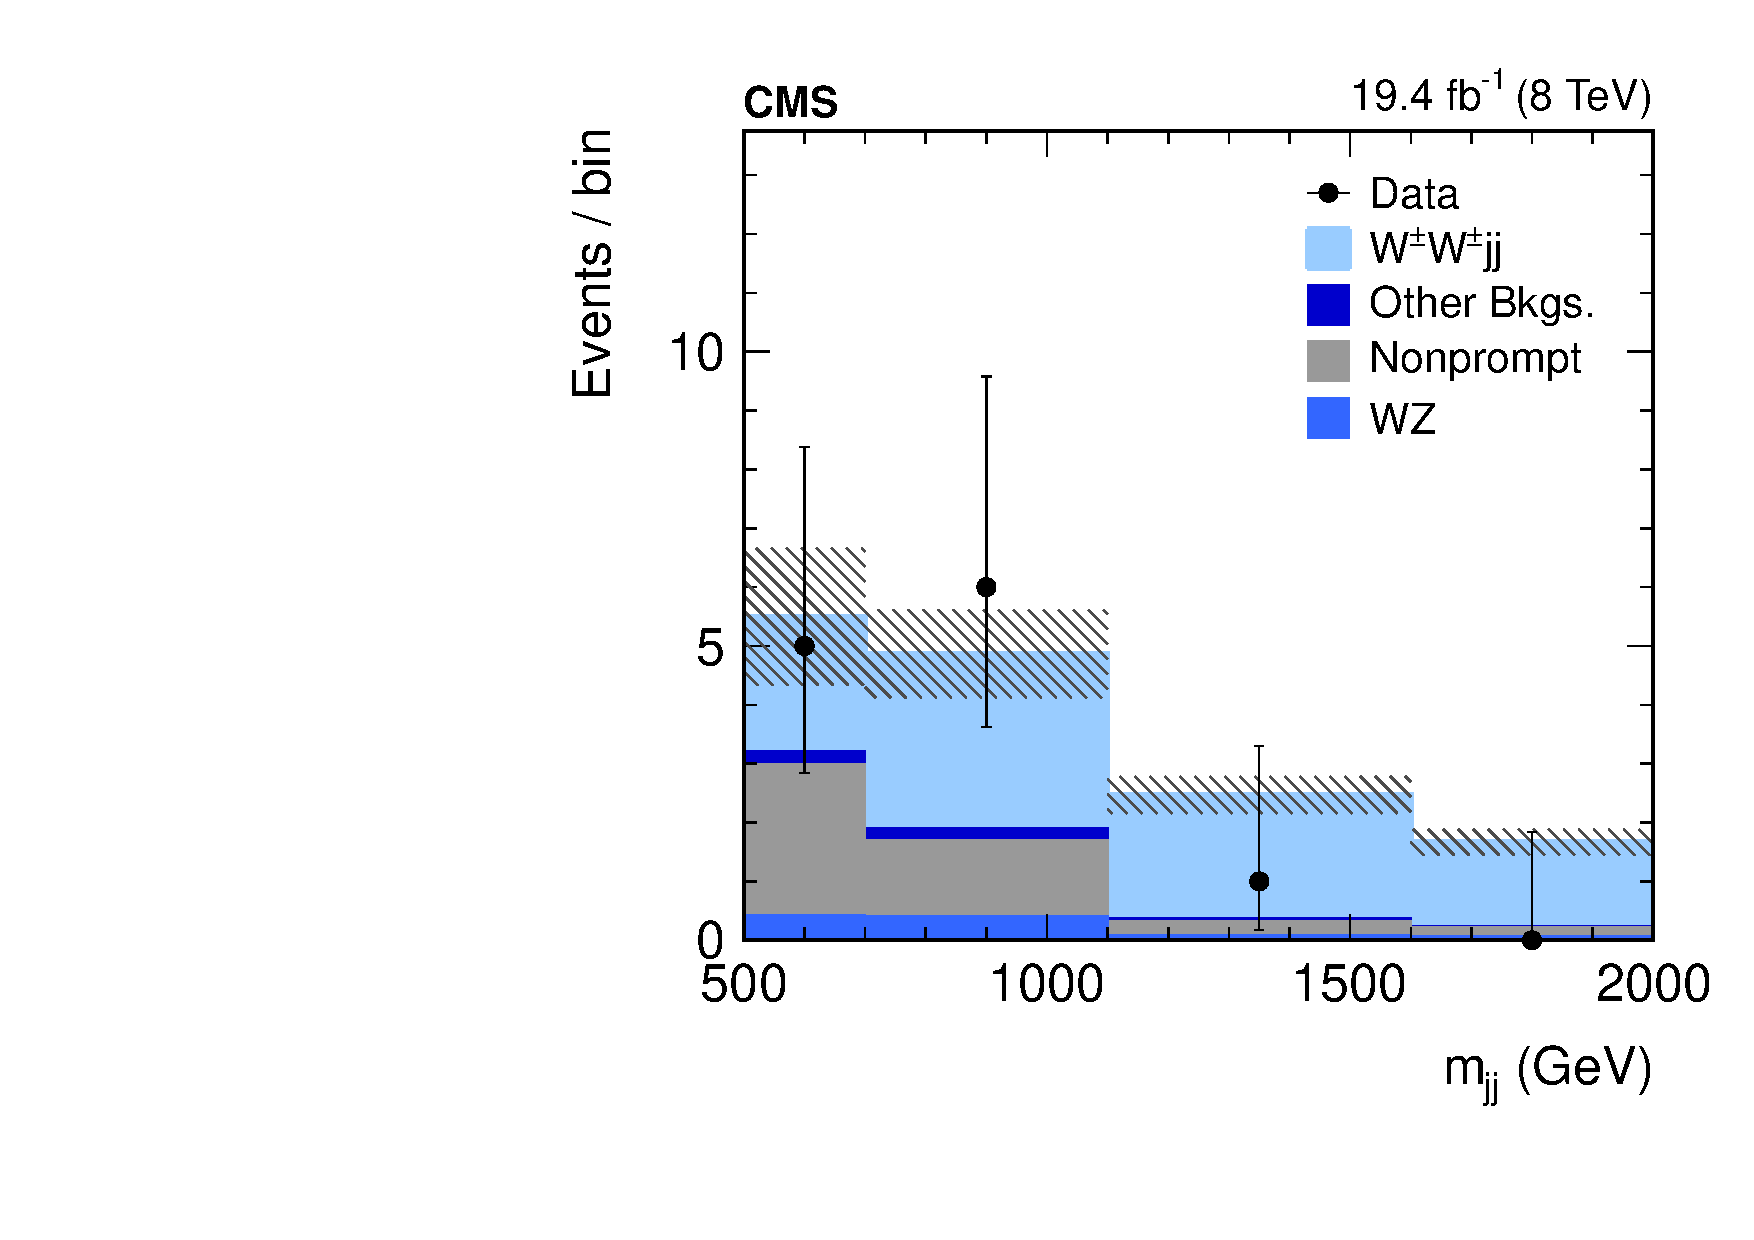
\includegraphics[width=0.45\textwidth]{figures/ss-exclboson-ww-ss-cms8tev.pdf}
    \caption{
    Left: Dijet invariant mass distribution of $W^{\pm} W^{\pm} jj$ candidates selected by ATLAS~\cite{Aad:2014zda}.  The inclusive signal region is indicated by the arrow.
    Right: Dijet invariant mass distribution of $W^{\pm} W^{\pm} jj$ candidates selected by CMS~\cite{Khachatryan:2014sta}.  }
    \label{fig:ss-exclboson-ww-ss}
\end{figure}


\subsection{Z AFB and sin thetaW}
%ATLAS weak mixing angle~\cite{Aad:2015uau}

In the electroweak theory the weak mixing angle $\theta_W$ is a free
parameter indicating the degree of mixing between $SU(2)_L$ and
$U(1)_Y$ neutral gauge bosons upon electroweak symmetry breaking to
obtain the physical neutral gauge bosons $\gamma$ and $\Zzero$.
Experimentally, it is typically measured as $\sin^2\theta_W$ via
angular distributions in fermion pair production; it has been most
precisely measured at the LEP 1 and SLD experiments via fermion pair
production at the $\Zzero$ pole, yielding a combined value of
$0.23153\pm0.00016$~\cite{ALEPH:2005ab}. In the standard model it is
related to the gauge boson masses at tree level by $1-m_W^2/m_Z^2$ and
modified by higher-order loop corrections, including contributions
from Higgs boson loops; the effective angle measured upon introducing
loop corrections is denoted as $\sin^2\theta^{eff}_{W}$. The recent
high-precision Higgs boson mass measurement at the LHC combined with
other electroweak measurements can be used to predict a value for
$\sin^2\theta^{eff}_{W}$ of $0.23149 \pm 0.00007$~\cite{Baak:2014ora},
motivating an improvement upon the direct experimental measurement
precision by a factor of two or more at the LHC to constrain the
electroweak theory further.

At a hadron collider, fermion pair production at and around the $\Zzero$
pole is measured in the process
$q\bar{q}\rightarrow \gamma^*/Z \rightarrow \ell^+\ell^-$, where the
differential scattering cross section is characterized by
$d^3\sigma/dm \ dy \ d\cos\theta = A(m,y)(1+\cos^2\theta) +
B(m,y)\cos\theta$, where $m$ is the final state lepton pair mass, $y$
is the lepton pair rapidity, and $\cos\theta$ is the polar angle of
the positive lepton with respect to the quark direction. A
non-vanishing forward-backward asymmetry in this angle, $A_{FB}(m,y) =
3B(m,y)/8A(m,y)$, arises from interference between vector and
axial-vector currents; the portion of $A_{FB}(m,y)$ corresponding to
self-interference of the $\Zzero$ boson currents is directly sensitive to
$\sin^2\theta^{eff}_{W}$.

In hadron collisions, the quark direction is ambiguous, as it may
originate from either incoming hadron and have unknown transverse
momentum. The impact of quark transverse momentum on the
forward-backward assignment is minimized by defining the quark
direction to be the difference between the forward-going and
backward-going hadron momentum vectors in the lepton pair rest frame,
as originally suggested by Collins and Soper~\cite{Collins:1977iv};
this angle is typically denoted as $\cos\theta^*$. In proton-proton
collisions, the ambiguity due to quark origination is an irreducible
dilution in $A_{FB}$ which is strongest at low $|y|$ and decreasing at
higher $|y|$ where valence quark/sea anti-quark annihilation is
predominant; measurements of $A_{FB}(m,y)$ at high-$|y|$ are therefore
intrinsically more sensitive to the undiluted value and have smaller
theory uncertainties related to PDFs.  In proton--anti-proton
collisions, valence quark/valence anti-quark annihilation
predominates, and so dilution and its associated uncertainties are
vastly reduced, making the Tevatron experimental
measurements~\cite{Aaltonen:2016nuy,Aaltonen:2014loa,Abazov:2014jti} a
competitive alternative to the LHC for current data samples. Three LHC
experiments have measured $\sin^2\theta^{eff}_{W}$: an initial
exploratory measurement by CMS at 7 TeV~\cite{Chatrchyan:2011ya}, a
measurement by ATLAS with all 7 TeV data~\cite{Aad:2015uau}, and a
measurement by LHCb~\cite{Alves:2008zz,Aaij:2014jba} with all 7 and 8
TeV data~\cite{Aaij:2015lka}.

The ATLAS measurement was performed with three different samples: muon
pairs with $\pt > 20$ GeV and $|\eta| < 2.4$; electron pairs with $E_T
> 25$ GeV and $|\eta| < 2.47$; and electron pairs with $E_T > 25$ GeV
where one has $|\eta| < 2.47$ and the other has $2.5 < |\eta| < 4.9$.
In the last case the forward electron is identified with calorimeters
alone, still the resulting pairs have a signal purity at the
$\Zzero$ pole of 95\%.  The data in each sample $i$ are binned in mass, and
the raw measured angular asymmetry in that region of phase space,
$A^{\rm meas}_{FB, i}(m)$, is computed from counting forward
($\cos\theta^* > 0$) and backward ($\cos\theta^* < 0$) candidates
after background subtraction.  Each $A_{FB,i}$ is used to extract
$\sin^2\theta^{eff}_{W}$ via a binned $\chi^2$ fit of
LO \texttt{PYTHIA} templates of different mixing angle values to the
data.  Figure~\ref{fig:ss-precision-afb-atlas-cf} shows the
$\cos\theta^*$ distribution for selected central-forward electron
pairs; an asymmetry between forward and backward angles is visually
evident.  Figure~\ref{fig:ss-precision-afb-atlas-cf} also show the
resulting $A^{\rm meas}_{FB}(m)$, alongside the best-fit predictions
from LO \texttt{PYTHIA} and NLO \texttt{POWHEG}.  The three samples
give consistent values for $\sin^2\theta^{eff}_{W}$ and are combined
to give a value of $0.2308 \pm 0.0005\textrm{(stat.)} \pm
0.0006\textrm{(syst.)} \pm 0.0009\textrm{(PDF)}$, where the last term
denotes the leading uncertainty in $\sin^2\theta^{eff}_{W}$ from
uncertainties in specially prepared LO PDFs consistent with the LO
PYTHIA template generation and 7 TeV ATLAS $W$ and $\Zzero$ data
(ATLAS-epWZ12 LO)~\cite{Aad:2011dm}.  A general feature of precision
electroweak measurements at the LHC is the predominance of PDF
uncertainties, requiring simultaneous PDF measurement with the
parameter of interest to obtain the best precision.  Other leading
systematic uncertainties are the lepton energy scale and MC template
statistics, which will improve with larger data sets.

The LHCb measurement employs a very similar technique.  They select
muon pairs with $\pt > 20$ GeV, $60 < m_{\mu\mu} < 160$ GeV, and $2.0
< |\eta| < 4.5$, with a signal mass resolution and purity similar to
ATLAS but in a more forward, and therefore more sensitive, $\Zzero$
production region.  LHCb operational instantaneous luminosity is
limited to the range $2-4\times
10^{32}\textrm{cm}^{-2}\textrm{s}^{-1}$, however, so the sample size
is limited to $1\;\fb^{-1}$ at 7~TeV and $2\;\fb^{-1}$ at 8 TeV.  The
data are binned in mass and $A_{FB}(m)$ is computed for their
acceptance, and then subsequently unfolded to account for mass
resolution effects. Figure~\ref{fig:ss-precision-afb-lhcb} shows the
unfolded $A_{FB}$ distribution at 8 TeV compared with NLO predictions
from \texttt{POWHEG-BOX}.  The unfolded $A_{FB}(m)$ distribution is
used to extract $\sin^2\theta^{eff}_{W}$ via a $\chi^2$ fit
of \texttt{POWHEG-BOX} templates of different mixing angle values to
the data.  They measure $\sin^2\theta^{eff}_{W} = 0.23142 \pm
0.00073 \textrm{(stat.)} \pm 0.00052 \textrm{(syst.)} \pm
0.00056 \textrm{(th.)}$, where the last term denotes uncertainties
from theoretical modelling ingredients, predominantly PDFs.  The PDF
uncertainties are evaluated from QCD+QED NLO NNPDF
2.3~\cite{Ball:2013hta,Ball:2012cx}, which, similar to the ATLAS PDF,
includes 7 TeV electroweak production data from the LHC.  In contrast
to the ATLAS result, the LHCb measurement statistically limited, but
has 30\% smaller theoretical uncertainties due to better understood
PDF uncertainties in the more forward production region.  In both
experiments, the impact of correctly modelling QED final state
radiation and higher-order electroweak corrections was studied via
comparison between different contemporary calculations, including
\texttt{PHOTOS}~\cite{Golonka:2005pn} and \texttt{PHOTONS++}~\cite{Schonherr:2008av} for
QED radiation, and \texttt{FEWZ}, \texttt{HORACE}~\cite{CarloniCalame:2007cd}, and
\texttt{POWHEG-BOX} for electroweak corrections.  The uncertainty associated
with these corrections is of order 0.1\% and sub-leading compared to
PDFs.

A comparison of experimental measurements of
$\sin^2\theta^{eff}_{W}$~\cite{Aaltonen:2016nuy} is shown in
Figure~\ref{fig:ss-precision-summary-sin2thetaw}.  The best single
measurements from the Tevatron are more than twice as precise as the
best measurements from the LHC, and the separate $A^{0,b}_{FB}$ and
$A_{l}$ results from $e^+e^-$ collisions are more than four times as
precise.  There are reasonable prospects for the LHC experiments
eventually surpassing these: ATLAS and CMS are expected to have
superior statistical uncertainties by the end of Run 2, and all of the
systematic and PDF uncertainties are expected to improve as well with
larger electroweak data samples.

%CMS Drell--Yan AFB 7 \TeV~\cite{Chatrchyan:2012dc}
%CMS Drell--Yan AFB 8 \TeV (CMS-PAS-SMP-14-004, to be published)
\begin{figure}[p]
    \centering
    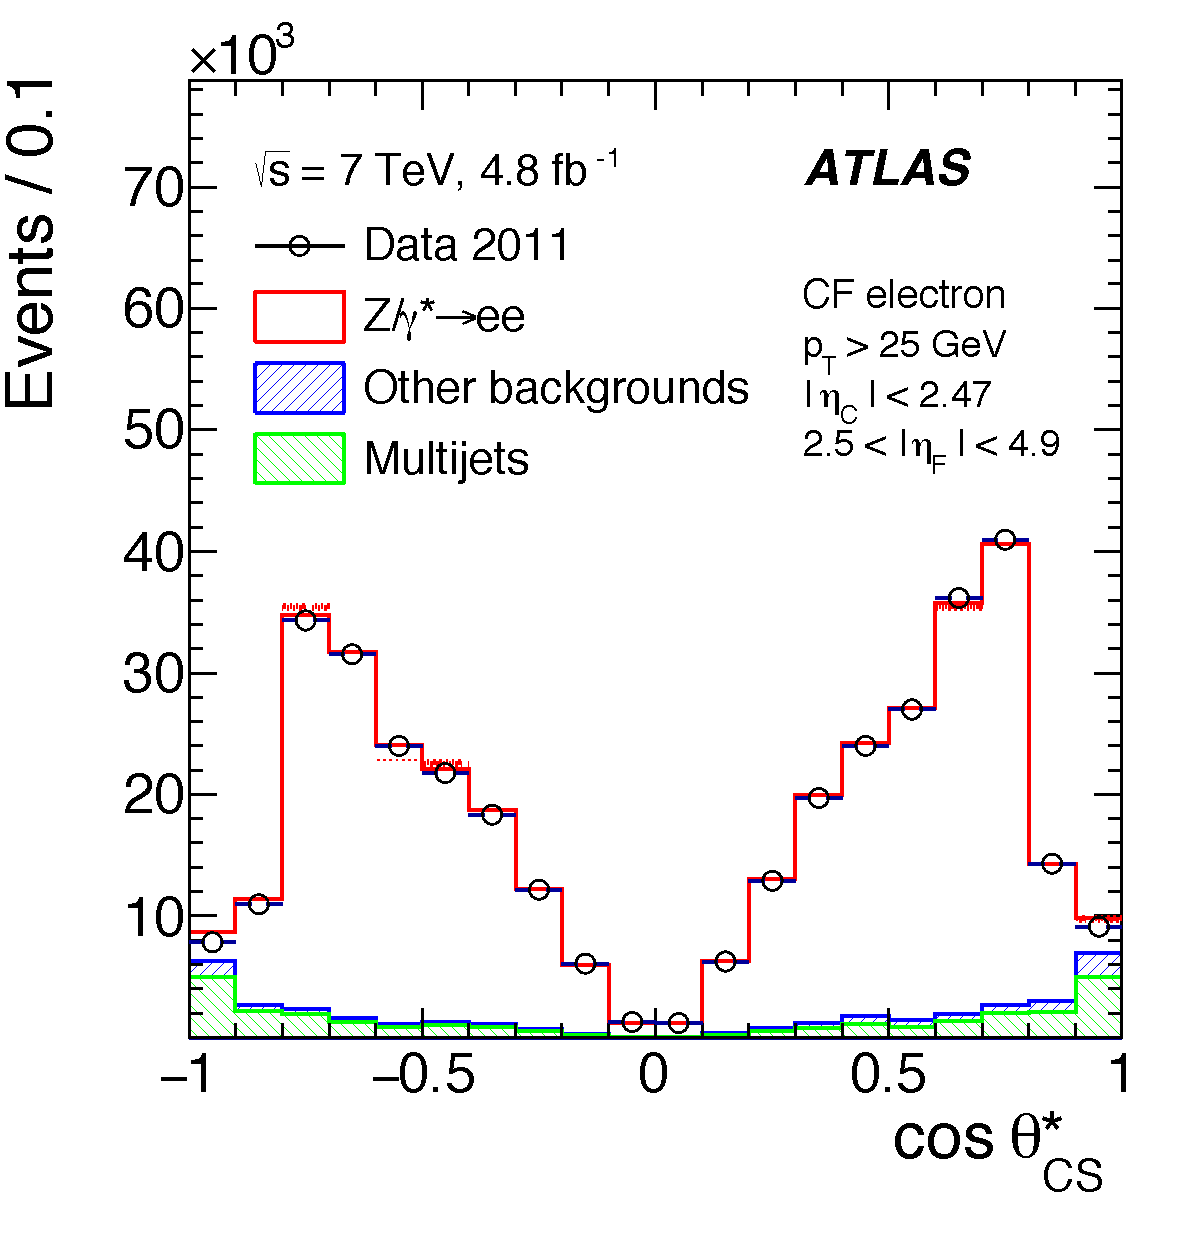
\includegraphics[width=0.45\textwidth]{figures/ss-precision-afb-atlas-cf-ct.pdf}
    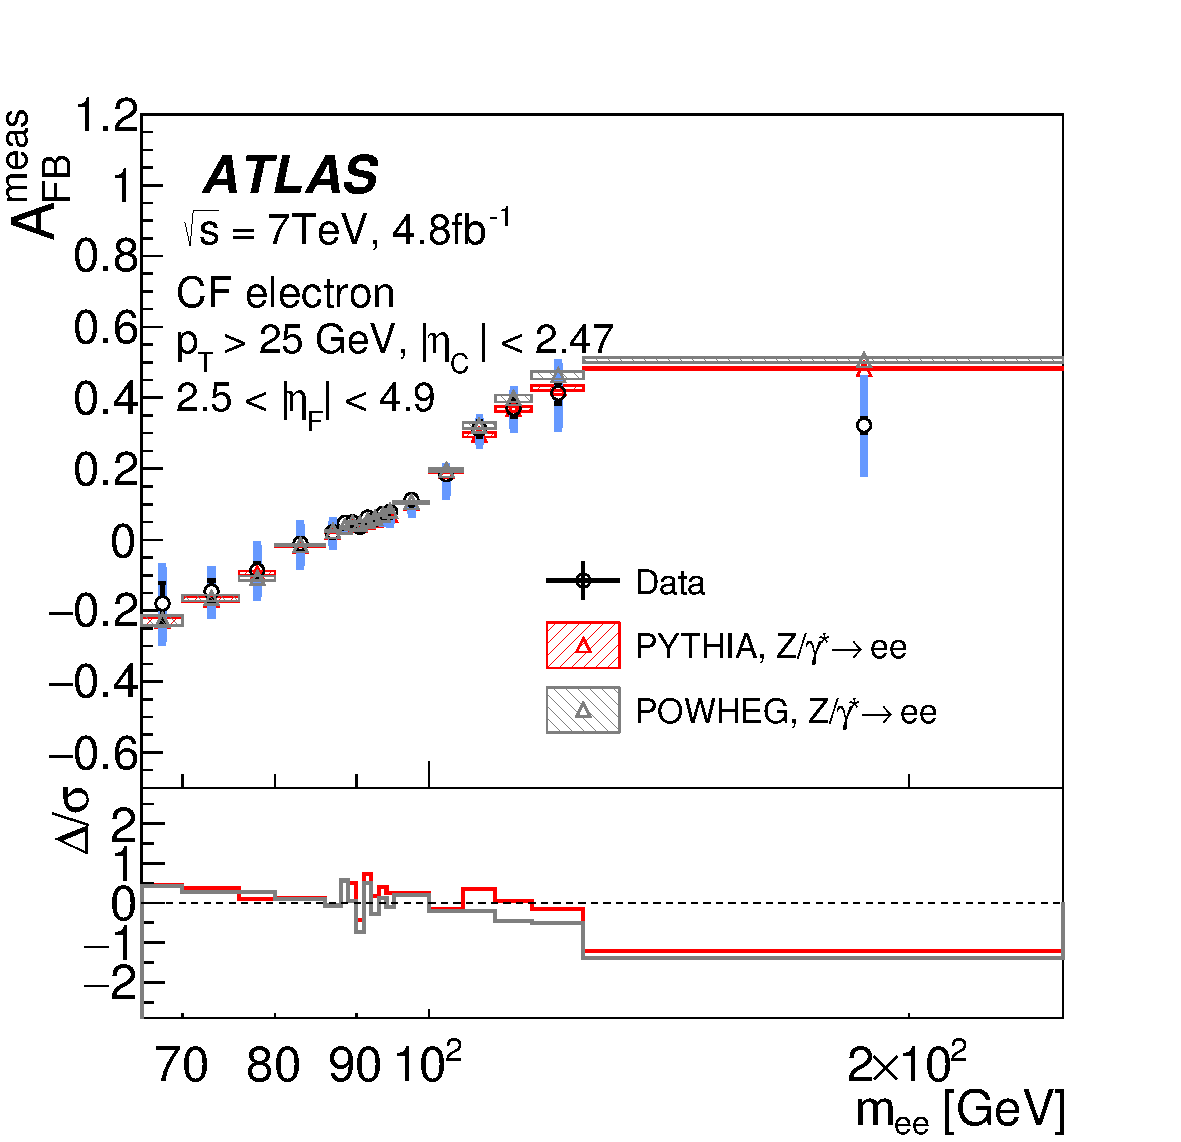
\includegraphics[width=0.45\textwidth]{figures/ss-precision-afb-atlas-cf-afb.pdf}
    \caption{
    From the ATLAS analysis of the full 7 TeV dataset~\cite{Aad:2015uau} on the left: The $\cos\theta^*$ distribution for selected central-forward electron pairs, compared with MC predictions.
    Right: $A^{\rm meas}_{FB}(m)$ for central-forward electron pairs, compared with MC predictions using the best fit $\sin^2\theta^{eff}_{W}$.}
    \label{fig:ss-precision-afb-atlas-cf}
\end{figure}

\begin{figure}[p]
    \centering
    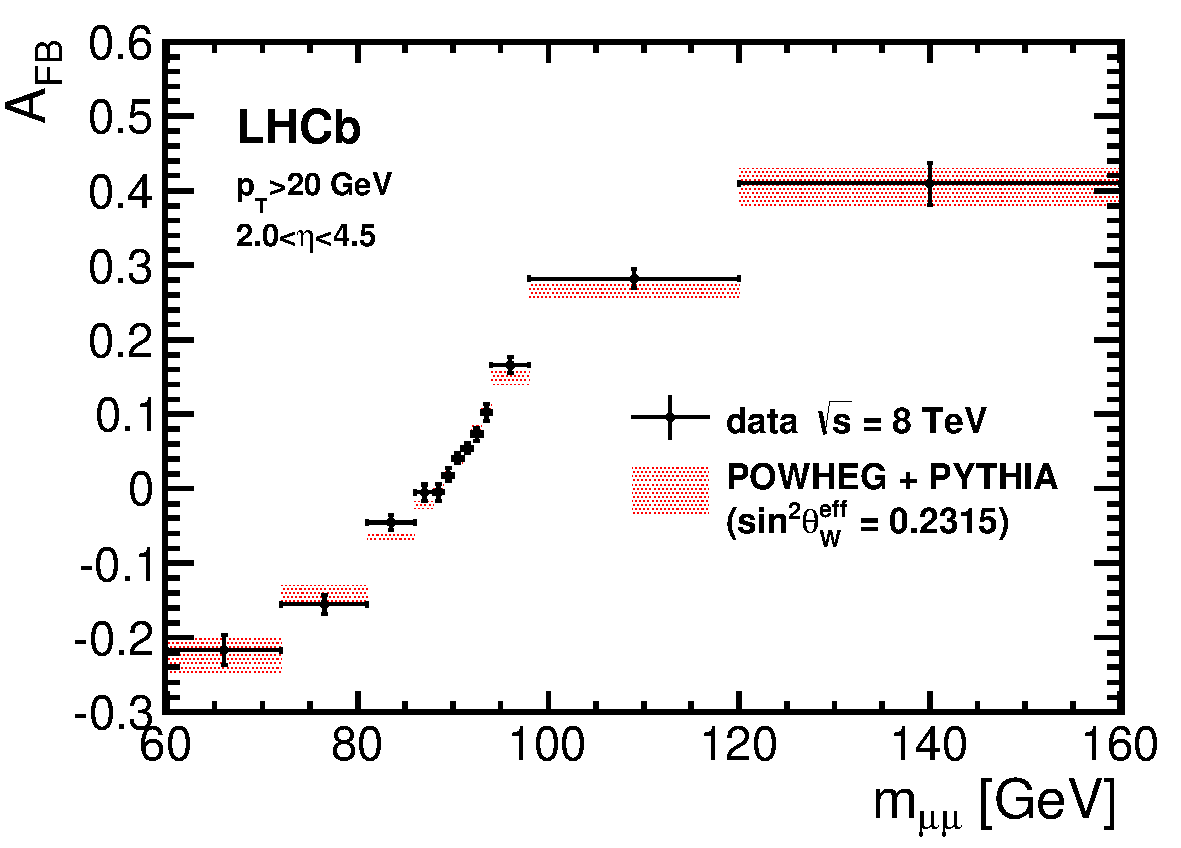
\includegraphics[height=0.3\textheight]{figures/ss-precision-afb-lhcb.pdf}
    \caption{The
unfolded $A_{FB}$ distribution from LHCb 8 TeV data , as a function of di-muon mass, compared with NLO predictions from \texttt{POWHEG-BOX}~\cite{Aaij:2015lka}.
    }
    \label{fig:ss-precision-afb-lhcb}
\end{figure}

\begin{figure}[p]
    \centering
    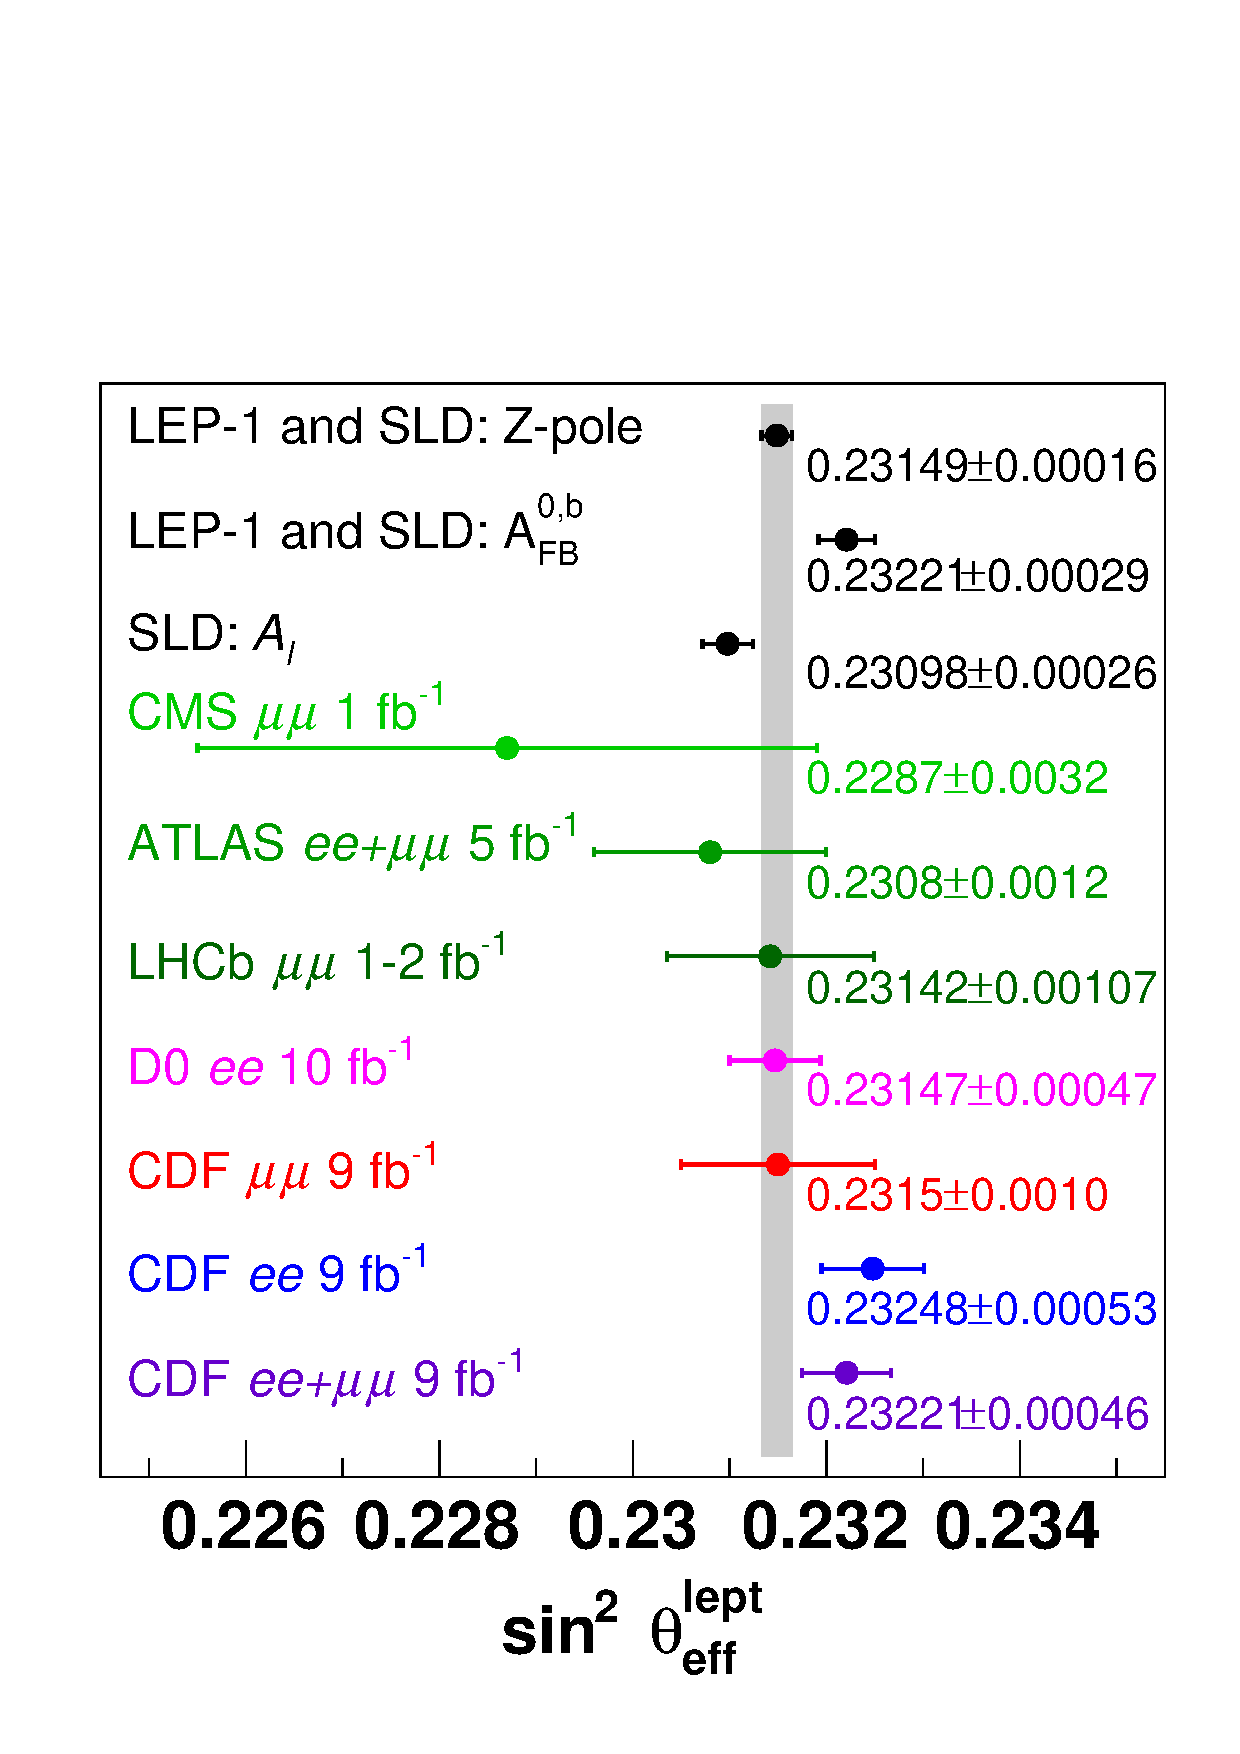
\includegraphics[height=0.3\textheight]{figures/ss-precision-summary-sin2thetaw.pdf}
    \caption{Comparison of experimental measurements of
$\sin^2\theta^{eff}_{W}$~\cite{Aaltonen:2016nuy}.}
    \label{fig:ss-precision-summary-sin2thetaw}
\end{figure}




\subsection{W mass}

\section{Summary}
%Summary & Outlook
The ATLAS and CMS experiments at the LHC have published a first set of electroweak measurements with the 
run-1 data-sets at a collision energy of 7\;\TeV and 8\;\TeV,
%, and some first measurements with run-2 data at $\rts=13\TeV$. 
probing the electroweak sector at the hitherto highest available scales.
%DY
We started with the discussion of precision measurents of Drell-Yan production, a well understood electroweak
process that in turn is used to validate theoretical calculations with higher order corrections in
$\alpha_s$ and the PDF's of the proton. The total and differential cross section measurements help to 
reduce the theoretical cross section uncertainties of multi-boson processes, which are generally of the same order as the current
experimental uncertainties.  
%diboson
We reviewed the set of results available so far on inclusive di-boson production at the LHC. All inclusive di-boson final states
($\WW,\WZ,\ZZ,\Wg,\Zg$) have been observed and cross section measurements are available for collision energies of 7 TeV and 8 TeV. 
The complete set of measurements from both ATLAS and CMS including leptonic and semi-leptonic decay channels
is expected to be published towards the end of 2016.
%WWW+VBS
A highlight of the electroweak physics program at the LHC is the observation of electroweak production channels 
that became accessible for the first time, namely processes with 
three vector bosons in the final state, and vector boson scattering processes that are 
characterised by two forward jets and two vector bosons in the final state.

%aGC limits
For most total and fiducial cross section measurements with the full run-1 dataset the systematic uncertainties 
already limit the precision. The exception are processes with cross sections below a few fb, e.g. tri-boson producion. 
To probe the validity of the standard model at high partonic centre-of-mass energy, $\hat{s}$, the limits
set in the framework of anomalous gauge couplings are surpassing legacy measurements at LEP and the Tevatron,
and are expected to further improve with increases $\rts$ and integrated luminosity. 

%legacy run-1 results
The set of run-1 results once completed will present a unique legacy of electroweak precision results at 
$\rts$ values of 7 and 8 TeV.
%outlook
The run-2 analysis extend the energy range to $\rts=13\TeV$ 
and provide even more precise limits on anomalous gauge couplings. Potentially, 
the combination of ATLAS and CMS results will allow more stringent constraints. Also the combination
with Higgs measurements in the framework of EFT with shared anomalous coupling operators is being 
actively pursued and will allow a further reduction of the allowed parameter space. 
Precision measurements or first observations of more Tri-boson production and VBS processes will become possible with the full 
run-2 data set. 


 



%ATLAS~\cite{Aad:2008zzm}
%CDF~\cite{Abulencia:2005ix}
%CMS~\cite{CMSdetector}
%D0~\cite{Abazov:2005pn}
%LHCb~\cite{Alves:2008zz}

%CDF Z asymmetry muon~\cite{Aaltonen:2014loa}
%CDF Z asymmetry electron~\cite{Aaltonen:2013wcp}
%CDF W mass PRD~\cite{Aaltonen:2013vwa}
%CDF W mass PRL~\cite{Aaltonen:2012bp}

%D0 W asymmetry electron~\cite{Abazov:2013dsa}
%D0 W asymmetry muon~\cite{Abazov:2013rja}
%D0 W mass PRD~\cite{D0:2013jba}
%D0 W mass PRL~\cite{Abazov:2012bv}

%CDF+D0 W mass combination~\cite{Aaltonen:2013iut}

%Snowmass electroweak~\cite{Baak:2013fwa}

%Wmass PDF~\cite{Bozzi:2011ww}

\ack
Acknowledgments go here.

\bibliographystyle{iopart-num}
\bibliography{ewkrun1_master}

\end{document}
